%
% This file is part of RHexLib, 
%
% Copyright (c) 2001 The University of Michigan, its Regents,
% Fellows, Employees and Agents. All rights reserved, and distributed as
% free software under the following license.
% 
%  Redistribution and use in source and binary forms, with or without
% modification, are permitted provided that the following conditions are
% met:
% 
% 1) Redistributions of source code must retain the above copyright
% notice, this list of conditions, the following disclaimer and the
% file called "CREDITS" which accompanies this distribution.
% 
% 2) Redistributions in binary form must reproduce the above copyright
% notice, this list of conditions, the following disclaimer and the file
% called "CREDITS" which accompanies this distribution in the
% documentation and/or other materials provided with the distribution.
% 
% 3) Neither the name of the University of Michigan, Ann Arbor or the
% names of its contributors may be used to endorse or promote products
% derived from this software without specific prior written permission.
% 
% THIS SOFTWARE IS PROVIDED BY THE COPYRIGHT HOLDERS AND CONTRIBUTORS
% "AS IS" AND ANY EXPRESS OR IMPLIED WARRANTIES, INCLUDING, BUT NOT
% LIMITED TO, THE IMPLIED WARRANTIES OF MERCHANTABILITY AND FITNESS FOR
% A PARTICULAR PURPOSE ARE DISCLAIMED. IN NO EVENT SHALL THE REGENTS OR
% CONTRIBUTORS BE LIABLE FOR ANY DIRECT, INDIRECT, INCIDENTAL, SPECIAL,
% EXEMPLARY, OR CONSEQUENTIAL DAMAGES (INCLUDING, BUT NOT LIMITED TO,
% PROCUREMENT OF SUBSTITUTE GOODS OR SERVICES; LOSS OF USE, DATA, OR
% PROFITS; OR BUSINESS INTERRUPTION) HOWEVER CAUSED AND ON ANY THEORY OF
% LIABILITY, WHETHER IN CONTRACT, STRICT LIABILITY, OR TORT (INCLUDING
% NEGLIGENCE OR OTHERWISE) ARISING IN ANY WAY OUT OF THE USE OF THIS
% SOFTWARE, EVEN IF ADVISED OF THE POSSIBILITY OF SUCH DAMAGE.

%%%%%%%%%%%%%%%%%%%%%%%%%%%%%%%%%%%%%%%%%%%%%%%%%%%%%%%%%%%%%%%%%%%%%%
% $Id: body.tex,v 1.6 2001/07/20 00:41:11 ulucs Exp $
%
% RHexLib documentation main file.
%
% Created       : Uluc Saranli, 01/06/2001
% Last Modified : Uluc Saranli, 06/27/2001
%
%%%%%%%%%%%%%%%%%%%%%%%%%%%%%%%%%%%%%%%%%%%%%%%%%%%%%%%%%%%%%%%%%%%%%%

\listfiles
\documentclass[10pt, letterpaper]{book}

% ------------------------------------------------------- %
% Load needed packages ---------------------------------- %

\usepackage{graphics, epsfig, subfigure, array, hhline}
\usepackage{verbatim, moreverb}
\usepackage{float, rotating}
\usepackage{longtable}
\usepackage{amsmath}
\usepackage{makeidx}

%\pagestyle{plain}

% ------------------------------------------------------- %
% Page setup  ------------------------------------------- %

%\renewcommand{\baselinestretch}{0.9}

\setlength{\paperwidth}{8.5in}
\setlength{\paperheight}{11in}
\setlength{\textwidth}{6.0in} 
\setlength{\oddsidemargin}{0.2in}
\setlength{\evensidemargin}{0.2in} 
%\setlength{\columnsep}{0.375in}

%\setlength{\topmargin}{0.4in} 
\setlength{\textheight}{8.5in}
%\setlength{\headheight}{-0.2in} 
%\setlength{\headsep}{0.5in}
%\setlength{\parindent}{1pc}

%\pagestyle{empty}

% ------------------------------------------------------- %
% Read utility files ------------------------------------ %

%\input{uluchdr.tex}
%
% This file is part of RHexLib, 
%
% Copyright (c) 2001 The University of Michigan, its Regents,
% Fellows, Employees and Agents. All rights reserved, and distributed as
% free software under the following license.
% 
%  Redistribution and use in source and binary forms, with or without
% modification, are permitted provided that the following conditions are
% met:
% 
% 1) Redistributions of source code must retain the above copyright
% notice, this list of conditions, the following disclaimer and the
% file called "CREDITS" which accompanies this distribution.
% 
% 2) Redistributions in binary form must reproduce the above copyright
% notice, this list of conditions, the following disclaimer and the file
% called "CREDITS" which accompanies this distribution in the
% documentation and/or other materials provided with the distribution.
% 
% 3) Neither the name of the University of Michigan, Ann Arbor or the
% names of its contributors may be used to endorse or promote products
% derived from this software without specific prior written permission.
% 
% THIS SOFTWARE IS PROVIDED BY THE COPYRIGHT HOLDERS AND CONTRIBUTORS
% "AS IS" AND ANY EXPRESS OR IMPLIED WARRANTIES, INCLUDING, BUT NOT
% LIMITED TO, THE IMPLIED WARRANTIES OF MERCHANTABILITY AND FITNESS FOR
% A PARTICULAR PURPOSE ARE DISCLAIMED. IN NO EVENT SHALL THE REGENTS OR
% CONTRIBUTORS BE LIABLE FOR ANY DIRECT, INDIRECT, INCIDENTAL, SPECIAL,
% EXEMPLARY, OR CONSEQUENTIAL DAMAGES (INCLUDING, BUT NOT LIMITED TO,
% PROCUREMENT OF SUBSTITUTE GOODS OR SERVICES; LOSS OF USE, DATA, OR
% PROFITS; OR BUSINESS INTERRUPTION) HOWEVER CAUSED AND ON ANY THEORY OF
% LIABILITY, WHETHER IN CONTRACT, STRICT LIABILITY, OR TORT (INCLUDING
% NEGLIGENCE OR OTHERWISE) ARISING IN ANY WAY OUT OF THE USE OF THIS
% SOFTWARE, EVEN IF ADVISED OF THE POSSIBILITY OF SUCH DAMAGE.

%%%%%%%%%%%%%%%%%%%%%%%%%%%%%%%%%%%%%%%%%%%%%%%%%%%%%%%%%%%%%%%%%%%%%%
% $Id: environments.tex,v 1.4 2001/07/19 16:35:56 ulucs Exp $
%
%  This file defines LaTeX environments for various styles in the documentation
%
% Created       : Uluc Saranli, 01/06/2001
% Last Modified : Uluc Saranli, 06/27/2001
%
%%%%%%%%%%%%%%%%%%%%%%%%%%%%%%%%%%%%%%%%%%%%%%%%%%%%%%%%%%%%%%%%%%%%%%

% ------------------------------------------------------- %
% Environments for data types -------------------------%

% Width of the boxes used around various environments below -------- %
\def\codeboxwidth{5.9in}

% Commands to encapsulate a part of text in a box ------------------ %
\newbox\TextBox
\def\starttextbox{\global\setbox\TextBox\hbox\bgroup\ignorespaces}
\def\stoptextbox{\egroup}

% Environment for outputting data type definitions ----------------- %
%\newenvironment{datatype}
%  {\begin{center}
%      \starttextbox
%        \begin{tabular}{l}} {
%        \end{tabular}
%      \stoptextbox
%      \framebox[5.9in][l]{\box\TextBox}
%    \end{center}
%}
\newenvironment{datatype}
  {\begin{center}
      \begin{tabular}{|p{6.0in}|}\hline} {
       \hline\end{tabular}
    \end{center}}

% New float type for Program Source code listings ------------------ %
\floatstyle{boxed}
\floatname{codefloat}{Listing}
\newfloat{codefloat}{thp}{code}

% Verbatim environment for code segments. Usually used inside codefloat ------ %
\newenvironment{codesegment}
  {\verbatim}
  {\endverbatim}

% Environment for outputting function prototypes ------------------- %
%\newenvironment{prototype}
%  {\vspace{0.15in}\begin{center}
%      \starttextbox\tt
%        \begin{tabular}{l}} {
%        \end{tabular}
%      \stoptextbox
%      \framebox[\codeboxwidth][l]{\box\TextBox}
%   \end{center}}
\newenvironment{prototype}
  {\begin{itemize}\item
      \tt} {\end{itemize}}

\newenvironment{classdef}{\small \verbatim} {\endverbatim}

% Environment for module description header ------------------------ %
\newenvironment{moduleheader}
  {\begin{center}
      \begin{tabular}{| >{\bf \hfill} p{1.2in}p{4.4in}|}
        \hline} {
        \hline
      \end{tabular}
    \end{center}}
\newcommand{\classname}[1]{Class Name: & #1 \\}
\newcommand{\modulebase}[1]{Base Classes: & #1 \\}
\newcommand{\modulename}[1]{Module Name: & "#1" \\}
\newcommand{\moduleflags}[1]{Module Flags: & #1 \\}
\newcommand{\usedmodules}[1]{Used Modules: & #1 \\}
\newcommand{\mline}{}
\newcommand{\constructors}{{\bf Class constructors:}}
\newcommand{\localinterface}{{\bf Local interface:}}
\newcommand{\datatypes}{{\bf Data types:}}
\newcommand{\configsymbols}{{\bf Configuration Symbols:}}
\newcommand{\symbolitem}[1]{\item{#1}\index{Configuration symbols!#1}}
\newcommand{\symbolindex}[1]{\index{Configuration symbols!#1}}
\newcommand{\examplecode}{{\bf Example code:}}

% Definitions of Synopsis and Details headings --------------------- %
\newcommand{\detailsheading}
 {\par\vspace{0.15in}\noindent\hspace{0.3in}
   {\bf \large Details}\par}

\newcommand{\synopsisheading}
 {\par\vspace{0.15in}\noindent\hspace{0.3in}
   {\bf \large Synopsis}\par}

% Some useful macros for include, define and typedef statements ---- %
\newcommand{\typedefcmd}[1]{{\tt typedef #1}}
\newcommand{\includecmd}[1] {{\tt \#include #1}}
\newcommand{\definecmd}[1] {{\tt \#define #1}}



%
% This file is part of RHexLib, 
%
% Copyright (c) 2001 The University of Michigan, its Regents,
% Fellows, Employees and Agents. All rights reserved, and distributed as
% free software under the following license.
% 
%  Redistribution and use in source and binary forms, with or without
% modification, are permitted provided that the following conditions are
% met:
% 
% 1) Redistributions of source code must retain the above copyright
% notice, this list of conditions, the following disclaimer and the
% file called "CREDITS" which accompanies this distribution.
% 
% 2) Redistributions in binary form must reproduce the above copyright
% notice, this list of conditions, the following disclaimer and the file
% called "CREDITS" which accompanies this distribution in the
% documentation and/or other materials provided with the distribution.
% 
% 3) Neither the name of the University of Michigan, Ann Arbor or the
% names of its contributors may be used to endorse or promote products
% derived from this software without specific prior written permission.
% 
% THIS SOFTWARE IS PROVIDED BY THE COPYRIGHT HOLDERS AND CONTRIBUTORS
% "AS IS" AND ANY EXPRESS OR IMPLIED WARRANTIES, INCLUDING, BUT NOT
% LIMITED TO, THE IMPLIED WARRANTIES OF MERCHANTABILITY AND FITNESS FOR
% A PARTICULAR PURPOSE ARE DISCLAIMED. IN NO EVENT SHALL THE REGENTS OR
% CONTRIBUTORS BE LIABLE FOR ANY DIRECT, INDIRECT, INCIDENTAL, SPECIAL,
% EXEMPLARY, OR CONSEQUENTIAL DAMAGES (INCLUDING, BUT NOT LIMITED TO,
% PROCUREMENT OF SUBSTITUTE GOODS OR SERVICES; LOSS OF USE, DATA, OR
% PROFITS; OR BUSINESS INTERRUPTION) HOWEVER CAUSED AND ON ANY THEORY OF
% LIABILITY, WHETHER IN CONTRACT, STRICT LIABILITY, OR TORT (INCLUDING
% NEGLIGENCE OR OTHERWISE) ARISING IN ANY WAY OUT OF THE USE OF THIS
% SOFTWARE, EVEN IF ADVISED OF THE POSSIBILITY OF SUCH DAMAGE.

%%%%%%%%%%%%%%%%%%%%%%%%%%%%%%%%%%%%%%%%%%%%%%%%%%%%%%%%%%%%%%%%%%%%%%
% $Id: names.tex,v 1.4 2001/07/18 20:04:50 ulucs Exp $
%
%  This file defines LaTeX macros for all the class names, datatypes etc.
% in RHexLib
%
% Created       : Uluc Saranli, 01/06/2001
% Last Modified : Uluc Saranli, 06/27/2001
%
%%%%%%%%%%%%%%%%%%%%%%%%%%%%%%%%%%%%%%%%%%%%%%%%%%%%%%%%%%%%%%%%%%%%%%


% ------------------------------------------------------- %
% Library Name ------------------------------------------ %
\def \rhexlib {{RHexLib}}

% ------------------------------------------------------- %
% RHexLib header files ---------------------------------- %
\def \typeshh {``types.hh''}
\def \mmhh {``ModuleManager.hh''}
\def \Hardwarehh {``Hardware.hh''}

% ------------------------------------------------------- %
% Module Manager Class names -----------------------------%

\def \Module        {{\tt Module}}
\def \ModuleManager {{\tt ModuleManager}}

% ------------------------------------------------------- %
% Module Manager Member Functions ------------------------%
\def \initFN        {{\tt init()}}
\def \activateFN    {{\tt activate()}}
\def \deactivateFN  {{\tt deactivate()}}
\def \uninitFN      {{\tt uninit()}}
\def \updateFN      {{\tt update()}}

% ------------------------------------------------------- %
% Module Manager Definitions -----------------------------%

\def \ModuleInactive {{\tt MODULE\_INACTIVE}}
\def \ModuleActive   {{\tt MODULE\_ACTIVE}}

% ------------------------------------------------------- %
% Low Level Hardware inetrface Class names -------------- %

\def \Hardware      {{\tt Hardware}}
\def \EncoderHW     {{\tt EncoderHW}}
\def \AnalogHW      {{\tt AnalogHW}}
\def \DigitalHW     {{\tt DigitalHW}}
\def \TimerHW       {{\tt TimerHW}}
\def \AccelHW       {{\tt AccelHW}}
\def \GyroHW        {{\tt GyroHW}}
\def \PowerHW       {{\tt PowerHW}}
\def \SwitchHW      {{\tt SwitchHW}}
\def \DialHW        {{\tt DialHW}}
\def \DCMotorHW     {{\tt DCMotorHW}}

% ------------------------------------------------------- %
% Existing Module names --------------------------------- %

\def \EncoderReader   {{\tt EncoderReader}}
\def \AnalogOutput    {{\tt AnalogOutput}}
\def \SpeedFilter     {{\tt SpeedFilter}}
\def \StallSensor     {{\tt StallSensor}}
\def \SlopeEstimator  {{\tt SlopeEstimator}}
\def \PulseWidth      {{\tt PulseWidth}}
\def \MotorControl    {{\tt MotorControl}}
\def \PositionControl {{\tt PositionControl}}
\def \StateMachine    {{\tt StateMachine}}
\def \DataLogger      {{\tt DataLogger}}
\def \VirtualMotor    {{\tt VirtualMotor}}
\def \VirtualInput    {{\tt VirtualInput}}
\def \DataLogger      {{\tt DataLogger}}
\def \RHexLogger      {{\tt RHexLogger}}

% ------------------------------------------------------- %
% Controller Module names ------------------------------- %

\def \CalibMachine    {{\tt CalibMachine}}
\def \WalkMachine     {{\tt WalkMachine}}
\def \RHexWalker      {{\tt RHexWalker}}
\def \SitMachine      {{\tt SitMachine}}
\def \StandMachine    {{\tt StandMachine}}

% ------------------------------------------------------- %
% Utility class names ----------------------------------- %

\def \SymbolTable     {{\tt SymbolTable}}
\def \Tokenizer       {{\tt Tokenizer}}
\def \Profiler        {{\tt Profiler}}

% ------------------------------------------------------- %
% RHexLib data types ------------------------------------ %

\def \bool {{\tt bool}}

% Shortcut types %
\def \intb   {{\tt int8}}
\def \uintb  {{\tt uint8}}
\def \intw   {{\tt int16}}
\def \uintw  {{\tt uint16}}
\def \intdw  {{\tt int32}}
\def \uintdw {{\tt uint32}}
\def \intqw  {{\tt int64}}
\def \uintqw {{\tt uint64}}

\def \uint   {{\tt uint}}
\def \vast   {{\tt vast}}
\def \uvast  {{\tt uvast}}
\def \VastToLong {{\tt VAST\_TO\_LONG}}
\def \VastToDouble {{\tt VAST\_TO\_DOUBLE}}

\def \CLOCK  {{\tt CLOCK}}

\def \floats {{\tt floats}}
\def \strings {{\tt strings}}
\def \float {{\tt float}}

\def \ClocksPerSec {{\tt MM\_CLOCKS\_PER\_SEC}}
\def \ClockToLong {{\tt CLOCK\_TO\_LONG}}
\def \ClockToDouble {{\tt CLOCK\_TO\_DOUBLE}}
\def \ClockToSec {{\tt CLOCK\_TO\_SEC}}
\def \ClockToMin {{\tt CLOCK\_TO\_MIN}}
\def \ClockToHour {{\tt CLOCK\_TO\_HOUR}}
\def \SecToClock {{\tt SEC\_TO\_CLOCK}}
\def \MinToClock {{\tt MIN\_TO\_CLOCK}}
\def \HourToClock {{\tt HOUR\_TO\_CLOCK}}
\def \MPI {{\tt M\_PI}}

% Module manager data types */
\def \mmstep {{\tt MM\_STEP}}
\def \hwparam {{\tt HWParam\_t}}
\def \hwcalib {{\tt HWCalib\_t}}
\def \motortarget {{\tt MotorTarget\_t}}
\def \motorgains {{\tt MotorGains\_t}}


\makeindex

\begin{document}

\pagenumbering{roman}

% ------------------------------------------------------- %
% Begin: Title ------------------------------------------ %

\title{\bf {\Huge \rhexlib\ Programmer's Reference Manual}}
\author{
  \vspace{0.2in}\\
  {\Large Ulu\d{c} Saranli, Eric Klavins \vspace{0.3in} } \\
  Department of Electrical Engineering and Computer Science \\
  The University of Michigan \\
  Ann Arbor, MI 48109-2110, USA\\
  {\tt \{ulucs, klavins\}@eecs.umich.edu}}
\date{}
\maketitle

% End: Title -------------------------------------------- %
% ------------------------------------------------------- %

\thispagestyle{empty}

% ------------------------------------------------------- %
% Begin: Misc titles ------------------------------------ %

%\vspace{0.3in}
%\begin{center}
%  {\Large CSE Technical report: CSE-TR-436-00}
%\end{center}

% End: Misc titles -------------------------------------- %
% ------------------------------------------------------- %

\newpage

\tableofcontents

\newpage

\pagenumbering{arabic}

%
% This file is part of RHexLib, 
%
% Copyright (c) 2001 The University of Michigan, its Regents,
% Fellows, Employees and Agents. All rights reserved, and distributed as
% free software under the following license.
% 
%  Redistribution and use in source and binary forms, with or without
% modification, are permitted provided that the following conditions are
% met:
% 
% 1) Redistributions of source code must retain the above copyright
% notice, this list of conditions, the following disclaimer and the
% file called "CREDITS" which accompanies this distribution.
% 
% 2) Redistributions in binary form must reproduce the above copyright
% notice, this list of conditions, the following disclaimer and the file
% called "CREDITS" which accompanies this distribution in the
% documentation and/or other materials provided with the distribution.
% 
% 3) Neither the name of the University of Michigan, Ann Arbor or the
% names of its contributors may be used to endorse or promote products
% derived from this software without specific prior written permission.
% 
% THIS SOFTWARE IS PROVIDED BY THE COPYRIGHT HOLDERS AND CONTRIBUTORS
% "AS IS" AND ANY EXPRESS OR IMPLIED WARRANTIES, INCLUDING, BUT NOT
% LIMITED TO, THE IMPLIED WARRANTIES OF MERCHANTABILITY AND FITNESS FOR
% A PARTICULAR PURPOSE ARE DISCLAIMED. IN NO EVENT SHALL THE REGENTS OR
% CONTRIBUTORS BE LIABLE FOR ANY DIRECT, INDIRECT, INCIDENTAL, SPECIAL,
% EXEMPLARY, OR CONSEQUENTIAL DAMAGES (INCLUDING, BUT NOT LIMITED TO,
% PROCUREMENT OF SUBSTITUTE GOODS OR SERVICES; LOSS OF USE, DATA, OR
% PROFITS; OR BUSINESS INTERRUPTION) HOWEVER CAUSED AND ON ANY THEORY OF
% LIABILITY, WHETHER IN CONTRACT, STRICT LIABILITY, OR TORT (INCLUDING
% NEGLIGENCE OR OTHERWISE) ARISING IN ANY WAY OUT OF THE USE OF THIS
% SOFTWARE, EVEN IF ADVISED OF THE POSSIBILITY OF SUCH DAMAGE.

%%%%%%%%%%%%%%%%%%%%%%%%%%%%%%%%%%%%%%%%%%%%%%%%%%%%%%%%%%%%%%%%%%%%%%
% $Id: introduction.tex,v 1.3 2001/07/18 20:04:50 ulucs Exp $
%
% Created       : Uluc Saranli, 01/06/2001
% Last Modified : Uluc Saranli, 06/27/2001
%
%%%%%%%%%%%%%%%%%%%%%%%%%%%%%%%%%%%%%%%%%%%%%%%%%%%%%%%%%%%%%%%%%%%%%%

\chapter{Introduction}

\section{Overview}

RHexLib is a collection of software components and modules to run on the
RHex robot. It incorporates low level hardware access routines, motion
control functionality and high level controllers. It is designed to be
modular and functional on different versions of underlying hardware with
minimal code modifications.

Currently, RHexLib has four major packages:

\begin{enumerate}
\item{\bf RHexLib\_core}\par 
This package is a collection of core components and the most stable standard
set of controllers. It also incorporates all the low level hardware
libraries for different versions of the robot. The following list summarizes
the contents of this package.

\begin{itemize}

\item{The Module Manager : A static scheduler for
periodic tasks}

\item{Symbol Table facilities: Management of configuration files and access
to configuration symbols.}

\item{Data logging tools : Modules to manage runtime logging and
storage of data.}

\item{State Machine framework : Formal mechanisms for defining and executing
state machines.}

\item{Basic motion control tools : Motor position sensing, local PD and
torque control, generic motion profiling tools.}

\item{Basic RHex calibration : Modules to perform automatic actuator and
sensor calibration of the robot.}

\item{Basic RHex controllers : Standing, sitting, alternating tripod walking
and alternating triwheel gait controllers.}

\item{Framework for hardware access : An abstract  class interface to low level hardware.}

\item{Hardware libraries : Support for Michigan RHex, McGill RHex, interface
to SimSect++ simulation environment and a set of virtual free running
motors.}

\item{Various examples : Lots of examples, module and template controllers.}
\end{itemize}

The components in this package are unlikely to undergo any significant
changes. New releases of the library will possibly add new components or
improve the existing ones in a backwards compatible way.

\item{\bf SimSect++}\par

SimSect++ is a simulation package for RHex, developed by Uluc Saranli. This
package is a version of SimSect++, which works with RHexLib in a transparent
way to implement the ability of testing RHexLib code outside the robot
itself. Being a somewhat simplified model of the robot, the behavioral
results of thesimulation are not as accurate, but as a development
framework, it is invaluable.

\item{\bf RHexLib\_Michigan}\par
This package contains all the modules and examples as well as the common
demo executable for the Michigan development team. The components in this
library are not essential to RHexLib's existence.

The idea behind this institution specific package is to decouple the
experimental development efforts between different institutions and minimize
the impact of such development on others. As such, this local package is
less constraining than the core library, but still has some restrictions on
minimal functionality before admitting a component.

\item{\bf RHexLib\_McGill}\par
This package contains all the modules and examples as well as the common
demo executable for the McGill development team. Its structure is the same
as the Michigan local package.

The latest versions of each of these packages as well as this documentation
are available through {\tt rhex.sourceforge.net}.
\end{enumerate}

\section{About This Manual}

We start in Chapter \ref{sec:quickstart} with tutorials on many commonly
encountered tasks, with specific worked out examples. Chapter
\ref{sec:fundamentals} then details the fundamentals of the library,
including all the library specific data types. This is followed by a
detailed description of the module manager and related tools in Chapter
\ref{sec:modulemanager}, which constitutes the foundations of RHexLib.

Chapter \ref{sec:rhexlib_module_summary} then gives a detailed summary of
all the modules in the core library, followed by Chapter
\ref{sec:utilities}, a reference for the various utilities in the
library. Detailed descriptions of the standard hardware components supported
by the abstract Hardware base class are presented in Chapter
\ref{sec:hardware_interface}. Various implementations of this hardware
interface in different hardware libraries are then described in Chapter
\ref{sec:hardware_libraries}. 



%
% This file is part of RHexLib, 
%
% Copyright (c) 2001 The University of Michigan, its Regents,
% Fellows, Employees and Agents. All rights reserved, and distributed as
% free software under the following license.
% 
%  Redistribution and use in source and binary forms, with or without
% modification, are permitted provided that the following conditions are
% met:
% 
% 1) Redistributions of source code must retain the above copyright
% notice, this list of conditions, the following disclaimer and the
% file called "CREDITS" which accompanies this distribution.
% 
% 2) Redistributions in binary form must reproduce the above copyright
% notice, this list of conditions, the following disclaimer and the file
% called "CREDITS" which accompanies this distribution in the
% documentation and/or other materials provided with the distribution.
% 
% 3) Neither the name of the University of Michigan, Ann Arbor or the
% names of its contributors may be used to endorse or promote products
% derived from this software without specific prior written permission.
% 
% THIS SOFTWARE IS PROVIDED BY THE COPYRIGHT HOLDERS AND CONTRIBUTORS
% "AS IS" AND ANY EXPRESS OR IMPLIED WARRANTIES, INCLUDING, BUT NOT
% LIMITED TO, THE IMPLIED WARRANTIES OF MERCHANTABILITY AND FITNESS FOR
% A PARTICULAR PURPOSE ARE DISCLAIMED. IN NO EVENT SHALL THE REGENTS OR
% CONTRIBUTORS BE LIABLE FOR ANY DIRECT, INDIRECT, INCIDENTAL, SPECIAL,
% EXEMPLARY, OR CONSEQUENTIAL DAMAGES (INCLUDING, BUT NOT LIMITED TO,
% PROCUREMENT OF SUBSTITUTE GOODS OR SERVICES; LOSS OF USE, DATA, OR
% PROFITS; OR BUSINESS INTERRUPTION) HOWEVER CAUSED AND ON ANY THEORY OF
% LIABILITY, WHETHER IN CONTRACT, STRICT LIABILITY, OR TORT (INCLUDING
% NEGLIGENCE OR OTHERWISE) ARISING IN ANY WAY OUT OF THE USE OF THIS
% SOFTWARE, EVEN IF ADVISED OF THE POSSIBILITY OF SUCH DAMAGE.

%%%%%%%%%%%%%%%%%%%%%%%%%%%%%%%%%%%%%%%%%%%%%%%%%%%%%%%%%%%%%%%%%%%%%%
% $Id: quickstart.tex,v 1.12 2001/07/20 00:41:11 ulucs Exp $
%
% Created       : Uluc Saranli, 01/06/2001
% Last Modified : Uluc Saranli, 06/27/2001
%
%%%%%%%%%%%%%%%%%%%%%%%%%%%%%%%%%%%%%%%%%%%%%%%%%%%%%%%%%%%%%%%%%%%%%%

\chapter{Quick Start Tutorial}
\label{sec:quickstart}

\section{Library Installation}

This section describes the basic procedures for installing and configuring
RHexLib and the optional simulation components SimSect++ and Geomview. The
latest version of RHexLib and SimSect++ can be downloaded from {\tt
http://ai.eecs.umich.edu/RHex/Internal/RHexLibdetails.html}. Geomview can be
downloaded from {\tt http://geom.umn.edu}.

\subsection{System Requirements}

The current version of RHexLib works with both the Linux and QNX operating
systems. The Linux version requires the use of either the {\em virtual} or
{\em SimSect} hardware libraries to provide a simulated interface to the low
level functionality of RHex. The QNX version does not work with the SimSect
hardware library.

The current version of SimSect++ works only with Linux as it requires the
use of Geomview (which is only available under Unix) for visualization.

Geomview currently works only with Unix-like platforms. Please refer to {\tt
http://www.geomview.org} for information about development of this
visualization tool.

\subsection{Installing SimSect++}

\begin{itemize}
\item{{\bf Create the directory structure}

Create a directory {\tt RHex}, where RHexLib, SimSect++ and all the user
development directories will reside:

{\tt 
mkdir RHex \\
cd RHex
}}

\item{{\bf Uncompress the library distribution}

Under the directory {\tt RHex}, uncompress SimSect++.tar.gz with the
following commands:

{\tt
gzip -d ../SimSect++.tar.gz\\
tar -xvf ../SimSect++.tar
}

This will create a directory called {\tt SimSect++}, where the library
distribution will reside.}

\item{{\bf Configure environment variables}

If you are using {\tt tcsh} as your Unix shell, add the following lines to
the {\tt .cshrc} file in your home directory:

{\tt
setenv SIMSECT\_DIR \~{}/RHex/SimSect++
}

Also, execute this command in your current shell so that they immediately
take effect.

Similarly, if you are using {\tt bash} as your Unix shell, add the following
lines to your {\tt .bashrc} file in your home directory:

{\tt
export SIMSECT\_DIR=\~{}/RHex/SimSect++
}}

\item{{\bf Compile the library}

Compile the library using the following commands from within the SimSect++
directory:

{\tt
make depend \\
make clean \\
make
}

This will compile and create the SimSect++ integration engine and model
libraries and place links to them in {\tt SimSect++/lib}. Moreover, it will
also create a standalone SimSect hexapod model simulation executable in {\tt
SimSect++/bin} }.

\end{itemize}

\subsection{Installing Geomview}

Please refer to Geomview installation instructions in {\tt
  http://geom.umn.edu}.

\subsection{Installing RHexLib under Linux}

\begin{itemize}
\item{{\bf Create the directory structure}

Create a directory called {\tt RHex}, where RHexLib, SimSect++ and all the
user development directories will reside. Note that if you already installed
SimSect++, you will already have created this directory.

{\tt 
mkdir RHex \\
cd RHex
}}

\item{{\bf Uncompress the library distribution}

In the directory {\tt RHex}, uncompress RHexLib.tar.gz with the
following commands:

{\tt
gzip -d ../RHexLib.tar.gz\\
tar -xvf ../RHexLib.tar
}

This will create a directory called {\tt RHexLib}, where the library
distribution will reside.}

\item{{\bf Configure environment variables}

If you are using {\tt tcsh} as your Unix shell, add the following lines to
the {\tt .cshrc} file in your home directory:

{\tt
setenv RHEX\_DIR \~{}/RHex/RHexLib\\
setenv RHEX\_HARDWARE \_MICHIGAN\_
}

Also, execute these commands in your current shell so that they immediately
take effect.

Note that setting {\tt RHEX\_HARDWARE} to either {\tt \_MICHIGAN\_} or {\tt
\_MCGILL\_} will determine which hardware configuration will be used for the
example files in the library.

Similarly, if you are using {\tt bash} as your Unix shell, add the following
lines to your {\tt .bashrc} file in your home directory:

{\tt
export RHEX\_DIR=\~{}/RHex/RHexLib\\
export RHEX\_HARDWARE=\_MICHIGAN\_
}}

\item{{\bf Compile the library}

Compile the library using the following commands:

{\tt
make depend \\
make clean \\
make all
}

This will compile and create the RHexLib core and hardware libraries and
place links to them in {\tt RHexLib/lib}. Moreover, it will also create
example executables in {\tt RHexLib/examples} }.

\end{itemize}

\subsection{Installing RHexLib under QNX}

The installation procedure under QNX is identical to the Linux installation
procedures of the preceding section. QNX will most likely have a bash-like
shell to start with, so use the bash specific instructions.

It is recommended that you create a specific user called {\tt rhex} and do
all the library compilation as that user rather than as the {\tt root}
user. Even though the executables will need to run as root to access
privileged IO instructions, development and compilation can (and should)
proceed without root privileges.

\subsection{Working with the Libraries} \label{sec:worklibraries}

RHexLib is designed to be a modular library, where users that need to create
controllers and design modules should not need to change any of the library
code. Consequently, instead of working in the library
distribution directory, each programmer should create a directory tree of
their own to do development. For example, a typical directory for the {\tt
  rhex} user on the robot would look like:\\

{\tt 
\noindent\~{}rhex \\
\~{}rhex/RHex \\
\~{}rhex/RHex/RHexLib \\
\~{}rhex/RHex/SimSect++ \\
\~{}rhex/RHex/UlucDevel \\
\~{}rhex/RHex/EricDevel
...
}\\

Developers should copy example files from {\tt RHexLib/examples} to their
own directory before making any changes or testing their controllers.

The directory {\tt RHexLib/tools} contains an example makefile called {\tt
Makefile.sample} to be used for compiling programs that use RHexLib. Users
can copy this file to their development directory and edit it to compile
their controllers:

{\tt 
\noindent cp RHexLib/tools/Makefile.sample UlucDevel/Makefile \\
}

You will need to make the following changes in the makefile before you can
compile programs:\\

{\tt
\noindent EXEC = example
}\\

This line specifies the name of the executable program that the compiler
will generate. The RHexLib makefile tools also expect to find a file with
the same base name and a {\tt .cc} extension in the same directory ({\tt
  example.cc}, in this case). Normally, this file is where {\tt main()} will 
be defined.\\

{\tt
\noindent SOURCES = SampleModule.cc ControlMachine.cc
}\\

This line specifies source files containing additional module, controller
and utilitie definitions that the user wants to link to the main
executable. It is always a good practice to separate components in the
controllers such as state machines, modules etc. into separate files and
specify them in the {\tt SOURCES} line. It will speed up compilation and
make it easier to navigate through your code.

If your sources require additional flags, they can be configured with an
additional line in the Makefile.\\

{\tt
\noindent AUXFLAGS = -I~rhex/RHex/UlucDevel/include
}\\

The RHexLib libraries that are required by your source must be included in
an additional statement. For example, for compilation on the Michigan RHex
the following line would need to be included in the Makefile.\\

{\tt
\noindent LIBS = librhex.a libmichiganhw.a libcommonhw.a libbase.a
}\\

Note that the order in which these libraries are specified is usually
important and can lead to compilation errors if not done properly. If
libraries which are not part of RHexLib (such as SimSect++ libraries {\tt
  libhexapod.a} {\tt libengine.a}), are to be linked, they must be indicated
in another statement as well.\\

{\tt
\noindent AUXLIBS = libhexapod.a libengine.a
}\\

Once {\tt Makefile} is modified appropriately, commands similar to the
following will create an executable.\\

{\tt
\noindent cd UlucDevel \\
make depend \\
make clean \\
make
}\\

Note that this sequence of commands deletes all precompiled object files,
and recompiles everything. In cases where small modifications are made to
the source files, the following command will be sufficient:\\

{\tt
\noindent make
}\\

\section{Basic Module Example: PrintModule}

This section describes the details of implementing a simple RHexLib program
which periodically displays the encoder counters. A similar example, {\tt
enc\_test\_mm}, can be found in the {\tt examples} directory of the source
distribution.

\subsection{The {\tt PrintModule} Class}

In RHexLib, any task that needs to be performed periodically is defined as 
a {\em Module}, more specifically as a class derived from the {\tt Module}
abstract base class. Below is a definition of the {\tt PrintModule} class,
which encapsulates the task of periodically reading and printing the encoder 
counter values.

\begin{codesegment}
#include "Hardware.hh"

class PrintModule : public Module {

public:
  PrintModule ( void ) : Module( "print", 0, false, false ) { };

  void init( void );
  void uninit( void ) { };
  void activate( void );
  void deactivate( void );
  void update( void );

private:
  Hardware *hardware;
};
\end{codesegment}

Note that each class derived from the virtual base class {\tt Module} must
define five methods: {\tt init()}, {\tt uninit()}, {\tt activate()}, {\tt
deactivate()} and {\tt update()}. These methods provide a a standard
interface to the {\tt ModuleManager} which, among other tasks, keeps a list
of all modules, manages their states, and calls the above methods at
appropriate times. In the case of {\tt PrintModule}, the {\tt uninit()}
method does not do anything, the rest of the methods are defined below.

An important detail to note is that the {\tt Module} class constructor takes
four arguments. The first two determine the {\em name} and {\em index} of
the module, which are used together to uniquely identify each module in the
system. The last two arguments determine the {\em type} of the module and
are explained in later chapters of this manual.

\subsection{The {\tt init()} method}

The {\tt init()} method of a module is called whenever the module is added
to the module manager's list with a call to the function {\tt
MMAddModule()}. The {\tt init} method is usually responsible for
initializing related hardware components and finding components and other
modules that are needed for the module's operation. In our example, the {\tt
PrintModule}, we will need access to the low level hardware interface, so
initialization involves acquiring a pointer to the interface object.

\begin{codesegment}
void PrintModule::init( void ) {
  hardware = MMGetHardware();
}
\end{codesegment}

The {\tt MMGetHardware()} function call returns a pointer to the currently
selected hardware interface object for the module manager. The selection of
this object usually takes place in {\tt main()} with a call to the function
{\tt MMChooseHardware()}.

\subsection{The {\tt activate()} method}

The {\tt activate()} method of a module is called whenever the module is
activated by the module manager via a call to either {\tt
MMActivateModule()} or the first call to {\tt MMGrabModule()}. This changes
the the module from the {\tt INACTIVE} state to the {\tt ACTIVE} state,
which means that the module manager will begin to periodically call the {\tt
update()} method of the module.

Activating a module usually involves making sure that all the components
needed for the task are active and operational. Moreover, necessary
initializations of the components must also be performed. For our example,
the {\tt PrintModule} will enable all the encoders using the hardware
interface.

\begin{codesegment}
void PrintModule::activate( void ) {
  int axis;

  for ( axis = 0; axis < 6; axis++ )
    hardware->encoders->enable( axis );
}
\end{codesegment}

\subsection{The {\tt deactivate()} method}

The {\tt deactivate()} method of a module is called whenever the module is
deactivated through a call to either {\tt MMDeactivateModule()} or the last
call to {\tt MMReleaseModule()}. This puts the module in the {\tt INACTIVE}
state, which means that the {\tt update()} method of the module will not be
called anymore.

For our example, upon deactivation, the {\tt PrintModule} will disable all
the encoders using the hardware interface.

\begin{codesegment}
void PrintModule::deactivate( void ) {
  int axis;

  for ( axis = 0; axis < 6; axis++ )
    hardware->encoders->disable( axis );
}
\end{codesegment}

\subsection{The {\tt update()} method}

The {\tt update()} method of a module is where its core functionality is
defined. When a module is in the {\tt ACTIVE} state, its {\tt update()}
function is called periodically by the module manager.

Our example module, the {\tt PrintModule}, will read the encoders and print
their contents in its {\tt update()} method. Moreover, it will also be
responsible for detecting keyboard input and exiting the program.

\begin{codesegment}
void  PrintModule::update ( void ) {
  int axis;

  printf( "Encoders: " );

  for ( axis = 0; axis < 6; axis++ )
    printf( "0x%04x, ", hw.encoders->read( axis ) );

  printf( "\n" );

  if ( kbhit() ) {
    MMMessage( "User interrupt: Shutting down!\n" );
    MMPowerOff( );speedd-speed
  }
}
\end{codesegment}

\section{Using PrintModule in a program}
 \label{sec:together}

What makes modules operational in RHexLib is the {\em Module Manager}. In
order to be operational, modules must be created as instatiations of the
class, and the module manager must be informed of its presence through the
{\tt MMAddModule()} library call. Moreover, it needs to be activated through
the {\tt MMActivateModule()} or {\tt MMGrabModule()} library functions in
order for its update() function to start being called periodically.

The library function {\tt MMMainLoop()} is the main entry point to the
module manager, and it never returns. It is usually called once from main(),
after all the desired modules are created and added to the module manager's
list. Once this function is called, the module manager takes control and
handles the periodic issues of module updates as well as other timing tasks.
Following a call to {\tt MMMainLoop()}, the only way to exit the program is
through the {\tt MMPowerOff()} function, from within one of the module
methods.

As such, there is a very typical way in which RHexLib programs are
built. The following program is the main entry point to our small example
and demonstrates how things are setup in a typical RHexLib program..
 
\begin{codesegment}

#include "ModuleManager.hh"
#include "SimSectHW.hh"

SimSectHW hw; // Create an instance of the SimSect hardware object.

int main( void ) {

  PrintModule pr; // Create an instance of the PrintModule module.

  // Let the module manager know about the current hardware
  MMChooseHardware( &hw );

  // Add and activate the print module
  MMAddModule( &pr, 10, 0, 10 );
  MMActivateModule( &pr );

  // Call the Module Manager main loop
  MMMainLoop();

  // Normally, the MMMainLoop() does not exit, so this point is never reached.
  return 0;
}
\end{codesegment}

As this code segment shows, the typical structure of {\tt main()} is as
follows:
\begin{itemize}
\item{Create an instance of the desired Hardware object}
\item{Call {\tt MMChooseHardware()} to inform the module manager the pointer
    to the hardware object.}
\item{Create and initialize all modules that will be used by the program.}
\item{Add the newly created modules to the module manager's list through
    {\tt MMAddModule()} function calls.}
\item{Activate the necessary modules through {\tt MMActivateModule()}
    function calls}
\item{Call {\tt MMMainLoop()}}
\end{itemize}

From then on, the module methods will determine the flow of the
execution. Note that at least one module needs to be activated before {\tt
MMMainLoop()} is called. Otherwise, the program will be stuck in an infinite
loop, and no module updates will take place.

An important detail is that the parameters of a module related to the
scheduling of its updates are determined by the {\tt MMAddModule( Module *,
  int period, int offset, int order )} function
call. It is hence possible to configure the {\em period}, the starting time
{\em offset} and the update {\em order} (in case of multiple updates
scheduled at the same time) of each module.

\section{Basic Controller Example: PushupController} \label{sec-pushup}

In this section we describe a more complicated module: a RHex-specific
controller which controls the robot to continuously do ``pushups''. It
demonstrates the simplest way of building a controller in RHexLib, how basic
motor control tasks are accomplished. It also shows some of the
configuration facilities commonly used in RHexLib.

This controller assumes that RHex is in the standing position to start
with. Starting there, it brings all the legs to a vertical position (making
the robot sit), waits there for a moment, and then stands up again,
restarting the cycle.

\subsection{The Module Definition}

Here we describe the details of how to define the {\tt PushupController}
module class and explain some of the components required by this
controller. Usually, the definitions of module classes in RHexLib are done
in separate header files, defining the interface of the module with the rest
of the library. In this case, the class definition will reside in {\tt
PushupController.hh}.

\begin{codesegment}
#include "ModuleManager.hh"
#include "PositionControl.hh"
#include "Profiler.hh"

class PushupController : public Module {

public:
  PushupController ( void )
    : Module( "pushupcontroller", 0, true, false ) { };

  // Module base class interface
  void  init ( void );
  void  uninit ( void ) { };
  void  activate ( void );
  void  deactivate ( void );
  void  update ( void );
\end{codesegment}

This part of the class definition is straightforward. We simply define the
standard module functions in a way similar to the previous example, the {\tt
PrintModule}. Once again, the name and index of the module are determined in
the definition of the class constructor, through the instatiation of the
base class {\tt Module}. Note also that in this case, all the module
functions except the uninit() method will be defined in the implementation
file {\tt PushupController.cc}.

Next we define a few private variables nad methods, local to {\tt
PushupController}.

\begin{codesegment}
private:

  PositionControl *control[6];
\end{codesegment}

These member variables will be pointers to the six different position
controller modules, associated with each one of the six legs. {\tt
PositionControl} modules implement basic proportional derivative(PD) control
feedback for all the motors in the system. Through their public interface,
our controller will be able to set the target positions for each leg,
updated every millisecond, commanding the legs perform the desired actions.

\begin{codesegment}
  MotorGains_t     oldGains[6];
\end{codesegment}

These member variables hold the PD gains that may have been in use by the
position controllers before the pushup controller is activated. When the
controller is deactivated, it will restore these gains to leave the position
controllers in their previous state. This is usually a good practice because
other components in the system might be expecting the PD gains to remain
unchanged for proper operation.

\begin{codesegment}
  Profiler         legProfiler;
\end{codesegment}

This member variable instantiates a {\tt Profiler} object, which is
responsible from generating the leg position as a function of time, also
called leg profile. Note that we only have one such object because, for the
pushup controller, all the legs are synchronized. Cconsequently, the desired
positions for all six legs will be the same at all times.

In RHexLib, the actual PD control of the leg motors and the generation of
the associated position profile are performed separately. Every millisecond,
our controller will ask the leg profiler the desired position for all the
legs. Then, it will set this new target on all six position
controllers. This scheme abstracts the generation of the desired leg
trajectories from the local PD feedback loop on the leg motors.

\begin{codesegment}
  void trackCurrentProfile( void );
\end{codesegment}

This utility method provides a facility to read the current value of the leg 
profiler and inform all the motor position controllers about the new target.

\begin{codesegment}
  double lowerTime;  // Time in seconds to lower the robot
  double chillTime;  // Time in seconds to chill, sitting down
  double standTime;  // Time in seconds to raise the robot up
  double waitTime;   // Time in seconds to wait standing up.
\end{codesegment}

These member variables determine how much time the controller should spend
in each of its stages. The pushup behavior can be decomposed into four
stages: lowering, chilling after sitting down, standing up and waiting in a
standing position. These variables determine how much time is spent in each
of these stages.

\begin{codesegment}
  int phase;
\end{codesegment}

This member variable indicates the current discrete ``phase'' of the
controllers. In implementing the aforementioned four different stages, the
pushup controller goes through six phases, where the controller actions are
defined as follows:

\begin{center}
\begin{tabular}{l}
0 : Starting to lower the robot \\
1 : Waiting for the robot to lower \\
2 : Wait for a while in the sitting position \\
3 : Starting to standup \\
4 : Waiting for the robot to standup \\
5 : Wait for a while in the standing position
\end{tabular}
\end{center}

Another way to write this controller is to use the {\tt StateMachine}
facilites of RHexLib. For this relatively simple example, we do not need the
power of state machines. If there were many more than six states, or if the
states were not visited in a simple cycle, or if the events that trigger
state transitions are were not so simple, state machines would probably make
the task simpler. {\tt StateMachine}s are covered later in this chapter and
elsewhere in this manual.

\begin{codesegment}
  double mark;
};
\end{codesegment}

This member variable is used to hold the state time of each phase in order
to switch to the next phase at appropriate times, determined by the values
of the timing member variables described above.

\subsection{The {\tt init()} Method}

There are two tasks usually performed by the {\tt init()} method of modules:
1) locate other modules that are going to be used; and 2) initialize member
variables by reading configuration information from a resource file..

With the function {\tt MMFindModule()}, RHexLib provides a means to acquire
a pointer to other module objects in the system. Almost all the
functionality of the library is implemented with modules, including low
level motor control, higher level behaviors such as walking, standing,
sitting, pronking as well as utilities such as logging data. Normally, in
{\tt main()}, all such modules to be used by an executable program are
``added'' to the system through calls to {\tt MMAddModule()}. The module
manager thus has a list of all these components, and can find modules by
their name and index, which are two of the parameters to the {\tt
MMFindModule()} function.

\begin{codesegment}
void PushupController::init( void ) {
  int i;

  for ( i = 0; i < 6; i ++ ) {
    if ( ( control[i] = ( PositionControl * ) 
           MMFindModule( POSITIONCONTROL_NAME, i )) == NULL)
      MMFatalError ( "PushupController::init", 
                     "Cannot find motor controller!" );
  }
\end{codesegment}

This part of the init method locates all six {\tt PositionControl}
modules. All of these six modules have the same name, defined in {\tt
StdModules.hh} as the macro {\tt POSITIONCONTROL\_NAME}, and their index
identifies which motor axis they correspond to. If {\tt MMFindModule()}
function call returns {\tt NULL}, indicating that the required module has
not yet been added to the module manager's list, a fatal error is generated,
and the program exits.

\begin{codesegment}
  lowerTime = MMGetFloatSymbol( "pushup_lower_time" , 1.0 );
  chillTime = MMGetFloatSymbol( "pushup_chill_time" , 0.3 );
  standTime = MMGetFloatSymbol( "pushup_stand_time" , 0.4 );
  waitTime = MMGetFloatSymbol( "pushup_wait_time" , 0.3 );
}
\end{codesegment}

The second part of the init method initializes the timing configuration of
the pushup machine. RHexLib maintains a global symbol table, where symbol
names are associated with either a floating point or a string value. Modules
in the system can access the table using {\tt MMGetFloatSymbol()} and {\tt
MMGetStringSymbol()} to retrieve the value of a particular symbol. These
functions also take a default value as an argument, to be returned if the
requested symbol cannot be found.

Usually, the symbol table is initialized by loading a ``configuration file''
using the {\tt MMReadConfig()} function in {\tt main()}. This configuration
file includes statements such as:

\begin{codesegment}
  pushup_lower_time = 0.9;
  pushup_chill_time = 0.2;
  pushup_stand_time = 0.5;
  pushup_wait_time = 0.2;
\end{codesegment}

which assign values to symbols. This mechanism provides means of
reconfiguring the behavior of controllers and modules without requiring that
the executable be recompiled.

\subsection{The {\tt activate()} Method}

The only modules used by the pushup controller are the motor position
controllers. Moreover, they are required throughout the whole operation of
the controller. As a consequence, the activate module method in this case is
responsible for requesting exclusive access to all six position controllers
and adjusting the PD gains appropriately.

\begin{codesegment}
void PushupController::activate( void ) {
  int          i;
  MotorGains_t gains;

  phase = 0;
\end{codesegment}

Every time the pushup controller is activated, it will start from phase 0:
starting to lower. The phase must be initialized in the activate method
because the same instantiation of this module may be activated more than
once (at different times) by different supervisory controllers.

\begin{codesegment}
  for ( i = 0; i < 6; i++ )
    MMGrabModule( control[i], this );
\end{codesegment}

This statement requests exclusive access to the motor position controller
modules whose pointers were acquired in the {\tt init} method. The functions
{\tt MMGrabModule()} and {\tt MMReleaseModule()} are thus used in pairs to
acquire and release the exclusive use of other modules in the system. They
should be used whenever the functionality of a module is needed to make sure
that the operation of other components in the system which might be using
the same modules is not disturbed.

In this context, there are two types of modules: {\tt SINGLE\_USER} and
{MULTI\_USER}. The type of a module is determined by its constructor. The
behavior of {\tt MMGrabModule()} is different for these two different types.

Single user modules can be grabbed by only one other module at a time. If a
second grab request is received, the system gives a fatal error and
exits. This mechanism makes sure that, for example, the motor position
controllers are not used by more than one entity at a time, which could
result in pretty chaotic behavior. Multi user modules can be grabbed as many
times as necessary.

Another feature of {\tt MMGrabModule()} is that the grabbed module
is also activated if it is not already active. Similarly, the {\tt
MMReleaseModule()} function deactivates the module if it has been
released as many times as it has been grabbed.  Hence, for multi user
modules, the first call to the grab function activates the module and the
last call to the release function deactivates the module.

\begin{codesegment}
  gains.kp = 5.0;
  gains.kd = 0.14;

  for ( i = 0; i < 6; i++ ) {
    control[i]->getGains( & oldGains[i] );
    control[i]->setGains( & gains );
  }
}
\end{codesegment}

This code segment saves the PD gains of the motor controllers and sets the
new gains to appropriate values for the pushup behavior.

\subsection{The {\tt deactivate()} Method}

The deactivate module method is usually responsible for releasing the
modules that have been grabbed in the activate method. In addition, it
usually restores their states to what they were before they were grabbed.

\begin{codesegment}
void PushupController::deactivate( void ) {
  int i;

  for ( i = 0; i < 6; i++ )
    control[i]->setGains( & oldGains[i] );
\end{codesegment}

This code segment restores the PD gains of the motor position controllers to 
their old values.

\begin{codesegment}
  for ( i = 0; i < 6; i++ )
    MMReleaseModule( control[i], this );
}
\end{codesegment}

Finally, all six motor position controllers are released to grant access to
anybody else who wants to use them.

\subsection{The {\tt update()} Method}

The update module method is where the bulk of the work is done for the
controller. All the other module methods are mainly for initialization and
clean integration with the rest of the system and do not much else.

Depending on the current phase of the controller, the update method, being
called once every millisecond, has to perform different tasks. As a
consequence, it ends up being a big case statement, implementing a primitive
state machine which linearly proceeds through 6 states (or phases). In later
sections, we will see more structured and formal ways of defining state
machines, which will allow the programmer to define much more complex
behaviors. Beyond 5 or 6 states, with transitions depending on events other
than simple timers, defining state machines through case statements quickly
becomes unelegant.

\begin{codesegment}
void PushupController::update( void ) {

  int           i;
  MotorTarget_t target;
  double        now = MMReadTime();
\end{codesegment}

This segment defines the local variables. An important function to note is
{\tt MMreadTime()}, which returns the current time in seconds.

\begin{codesegment}
  switch ( phase ) {
  case 0:   // Starting to lower the robot

    legProfiler.setup( SEC_TO_CLOCK(now), SEC_TO_CLOCK(now + lowerTime), 
                       0, M_PI / 2 );
\end{codesegment}

As described in the preceding sections, phase 0 in the pushup controller is
when the robot starts to lower. Hence, in this state, we initialize the leg
profile to bring the leg to a horizontal position and immediately proceed
with the next phase.

The {\tt setup(t1, t2, val2, val2)} method of the {\tt Profiler} class is
used to initialize a linear time trajectory for the leg between two angle
values. The resulting trajectory has the following functional form:

\begin{equation*}
f(t) = \left\{\begin{array}{l@{\hspace{0.3in}}l}
val_1 & t < t_1 \\
val_1 + {(t-t_1) (val_2-val_1)}/{t_2-t_1)} & t_1 \leq t \leq t_2 \\
val_2 & t > t_2 \\
\end{array}\right.
\end{equation*}

Note that this interface does not know anything about the $2 \pi$
periodicity of angles, and interprets $val_1$ and $val_2$ as real
numbers. The pushup controller, in order to lower the robot to the ground,
sets up a linear profile starting from 0 (vertical legs) and going to
$\pi/2$ (horizontal legs) in the amount of time configured in the init method.

\begin{codesegment}
    mark = now;
    phase = 1;
    break;
\end{codesegment}

This phase of execution also marks the current time to measure how much more 
the controller needs to wait before initiating the chilling phase. Also, the
assignment to the phase member variable transitions into phase 1, which
waits for the robot lowering to end.

\begin{codesegment}
  case 1:   // Waiting for the robot to lower

    if ( now < ( mark + lowerTime ) )
      trackCurrentProfile();
    else {
      mark = now;
      phase = 2;
    }
    break;
\end{codesegment}

During phase 1, the controller does not change the profile which has been
setup in phase 0. However, it reads the current target position from the
profile and commands the motors to go to the current target angle through
repeated calls to the {\tt trackCurrentProfile()} method (whose details are
explained later). When the legs reach their horizontal position
(i.e. when {\tt lowerTime} amount of time has elapsed), the controller
switches to phase 2.

\begin{codesegment}
  case 2:   // Wait for a while in the sitting position

    if ( now > ( mark + chillTime ) ) {
      mark = now;
      phase = 3;
    }
    break;
\end{codesegment}

During this phase, the controller simply waits for a configured amount of
time, without commanding new targets for the legs. Due to the fact that the
position control modules retain their latest assigned target, the legs
maintain their horizontal positions, chilling in a sitting down
position. Once again, note the use of the {\tt mark} member variable, which
is a typical way of handling time-based transitions between different
controller phases.

\begin{codesegment}
  case 3:   // Starting to standup

    legProfiler.setup( now, now + standTime, M_PI / 2, 0 );
    mark = now;
    phase = 4;

    break;
\end{codesegment}

Similar to phase 0, our controller next sets up a new leg trajectory in this
phase. This time, however, the legs are commanded to go from $\pi / 2$ to
$0$, effectively raising the robot to a standing position.

\begin{codesegment}
  case 4:   // Waiting for the robot to standup
    if ( now < ( mark + standTime ) )
      trackCurrentProfile();
    else {
      mark = now;
      phase = 5;
    }

    break;

  case 5:   // Wait for a while in the standing position
    if ( now > ( mark + waitTime ) ) {
      mark = now;
      phase = 0;
    }
    break;

  }
}
\end{codesegment}

Phases 4 and 5 perform exactly the same functionality as the phases 1 and 2, 
first tracking the leg profiles for standing up, and then waiting a little
while in a standing position. Note that the controller returns to phase 0
once done with phase 5, restarting the sequence by lowering the robot to the 
ground.

\subsection{The {\tt trackCurrentProfile()} Method}

As explained in the preceding sections, the commonly performed task of
reading the desired positions for the legs from the leg profiler and setting
the targets of the position controllers is done by this method.

\begin{codesegment}
void PushupController::trackCurrentProfile ( void ) {

  int i;
  MotorTarget_t target;

  target = legProfiler.getVal();

  // Command all 6 motor controllers to go to that position.
  for ( i = 0; i < 6; i++ )
    control[i]->setTarget ( & target );
}
\end{codesegment}

The data type {\tt MotorTarget\_t} holds the desired position, velocity and
acceleration for the motor, which is used by the local PD feedback
control. The leg profiler extracts this information from the functional form
given in the previous section, and returns it through its {\tt getVal()}
method. This target can then be directly passed into {\tt
PositionControl::setTarget()}.

\section{State Machines}

Next we illustrate another aspect of RHexLib which allows the programmer to
define discrete event driven controllers called {\em state machines}. We we
first build a very simple state machine, to illustrate the tools involved,
and then build a more complicated machine to show how the facility can be
used to supervise other controllers (which may themselves be state
machines).

\subsection{A Toy Machine}

We will first impliment the machine shown in Figure \ref{fig-toymachine}
which has two {\em states}, called {\tt stateOne} and {\tt stateTwo} and one
{\em event} called {\tt eventOne}. We will construct the machine so that it
starts in the first state and stays there for one second and then
transitions to the second state. RHexLib provides a perl script to set up
new state machine classes. The first step is to define a description file
called {\tt ToyMachine.dsc} which contains the same information that Figure
\ref{fig-toymachine} depicts graphically:

\begin{figure}[t]
\begin{center}
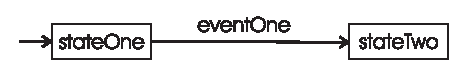
\epsfig{file=toymach.eps}
\caption{A simple state machine, called {\tt Toymachine}, which is implemented
in this section. \label{fig-toymachine}
}\end{center}
\end{figure}

\begin{codesegment}
  Transition stateOne eventOne stateTwo
  Initial stateOne
\end{codesegment}

\noindent This file specifies a State Machine module with two states and one transition. To
translate it into C++ code, we run the perl script {\tt sm-setup.pl} (for
``state machine setup'') as follows:

\medskip
\noindent{\tt > \$RHEX\_DIR/util/sm-setup.pl ToyMachine}
\medskip

\noindent This creates two generic files: {\tt ToyMachine.hh} and {\tt
ToyMachine.cc} to which we must add our own custom functionality. The first file
contains the definition of class {\tt ToyMachine} which is derived from the
virtual class {\tt StateMachine} which is derived from the virtual class {\tt
Module}. Thus a state machine is a kind of module, and therefore deals with the
Module Manager in much the same way as the modules we have already
encountered. However, the five virtual functions defined in the {\tt Module}
base class, and in particular the {\tt update()} method, are already defined in
any class that derives from {\tt StateMachine}. To give a state machine
interesting functionality, we must define the semantics of the states and
events.

First, look at {\tt ToyMachine.hh} which the perl script produced from the
{\*.dsc} file. It is as follows, except we have added a data variable called
{\tt mark} to the {\tt ToyMachine} class definition. We will use this
variable to {\em mark} the time at which the first state of the machine is
entered.

\begin{codesegment}
  #ifndef _TOYMACHINE_HH
  #define _TOYMACHINE_HH

  #include "ModuleManager.hh"
  #include "StateMachine.hh"

  class ToyMachine : public StateMachine {

    public:

      ToyMachine ( void );
      ~ToyMachine ( void );
      void init ( void );
      void activate ( void );
      void deactivate ( void );

    private:

      // events
      EventObject ( EventOne ) * eventOne;

      // states
      StateObject ( StateOne ) * stateOne;
      StateObject ( StateTwo ) * stateTwo;

      // data
      double mark;
  };

  #endif
\end{codesegment}

\noindent Note how the states and event are declared using the macros {\tt
  EventObject} and {\tt StateObject}. These macros, defined in {\tt
  Statemachine.hh}, declare new types whose scope is the {\tt ToyMachine}
  class. Thus the line

\begin{codesegment}
  EventObject ( EventOne ) * eventOne;
\end{codesegment}

\noindent does several things. First, it defines a new class {\tt EventOne}
which is derived from the virtual class {\tt Event}. Note that the scope of the
new class {\tt EventOne} does not extend beyond the {\tt ToyMachine}, thus,
other State Machines may also use the same class name without causing any
conflicts. Second, it declares this class a friend of class {\tt
ToyMachine}. And third, it sets {\tt eventOne} to be a pointer to an object of
class {\tt EventOne}. The {\tt StateObject} lines are similar.

Next, look at {\tt ToyMachine.cc}, also produced by the {\tt sm-setup.pl}
script. Here, the methods associated with the {\tt ToyMachine} class and the
state and event classes {\tt StateOne}, {\tt StateTwo} and {\tt EventOne}
and defined. This file is as follows:

\begin{codesegment}
  #include "ToyMachine.hh"

  #define OWNER ( ( ToyMachine * ) owner )

  // Events ------------------------------------------------------------
  bool ToyMachine::EventOne::check ( void ) { return false; }

  // States ------------------------------------------------------------
  void ToyMachine::StateOne::entry ( void ) {}
  void ToyMachine::StateOne::during ( void ) {}
  void ToyMachine::StateOne::exit ( void ) {}

  void ToyMachine::StateTwo::entry ( void ) {}
  void ToyMachine::StateTwo::during ( void ) {}
  void ToyMachine::StateTwo::exit ( void ) {}

  ToyMachine::ToyMachine ( void ) : StateMachine ( "toymachine" ) {

    // allocate events
    eventOne = new EventOne ( this );

    // allocate states
    stateOne = new StateOne ( this );
    stateTwo = new StateTwo ( this );

    // transitions
    Transition ( stateOne, eventOne, stateTwo );

    // the initial state
    initialize ( stateOne );

  } 

  ToyMachine::~ToyMachine ( void ) {

    if ( eventOne ) delete ( eventOne );
    if ( stateOne ) delete ( stateOne );
    if ( stateTwo ) delete ( stateTwo );

  }
 
  void ToyMachine::init ( void ) {

    StateMachine::init();

  }

  void ToyMachine::activate ( void ) {

    StateMachine::activate();

  }

  void ToyMachine::deactivate ( void ) {

    StateMachine::deactivate();

  }

\end{codesegment}

The constructor for the {\tt ToyMachine} class performs several steps. It sets
{\tt eventOne} to point to a new {\tt EventOne} object. Note that the
constructor to {\tt EventOne} requires a pointer (in this case, {\tt this}) to a
state machine class that ``owns'' the event. This will be used by the event's
method later to access the data (such as the datum {\tt mark} that we added
above) in the state machine that owns it. It then similarly sets the event
object pointers to point to new state objects. The next step sets up the
transitions in the state machine --- in this case there is only one
transition. The line

\begin{codesegment}
  // transitions
  Transition ( stateOne, eventOne, stateTwo );
\end{codesegment}

\noindent adds a {\em transition} or {\em arc} to the {\tt ToyMachine} being
constructed. The source state of the transition is {\tt stateOne}, the
destination state is {\tt stateTwo}. The event that {\em guards} the
transition from the source to the destination is {\em eventOne}. The last
step is to set up the initial state ({\tt stateOne}) of the state machine
and this is doen by the last line of the constructor.

The behavior of a {\tt ToyMachine} is as follows. When it becomes active, it
first calls the {\tt entry} method of its initial state (in this case of
{\tt stateOne}) and then continuously calls the {\tt update} method of this
state. The {\tt ToyMachine} also continuously checks the {\tt check} method
of {\tt eventOne} until it returns true. When this happens, it then calls the
{\tt exit} method of {\tt stateOne} and then then the {\tt entry} method of
{\tt stateTwo} and then continuously calls the {\tt update} function of {\tt
stateTwo}.

As it is, the script {\tt sm-setup.pl} has not put any meaning in the states
and event. It has made all the methods of {\tt stateOne} and {\tt stateTwo}
empty. And it has defined the {\tt check} method of {\tt eventOne} to always
return {\tt false}! Recall that we wanted {\tt stateOne} to be active for
one second and then for {\tt stateTwo} to be active. To arrange for this, we
first redefine the methods of {\tt stateOne} as follows:

\begin{codesegment}
  void ToyMachine::StateOne::entry ( void ) {

    OWNER->mark = MMReadTime();
    printf ( "State One Entered at Time %f\n", OWNER->mark );

  }

  void ToyMachine::StateOne::during ( void ) {}

  void ToyMachine::StateOne::exit ( void ) {
 
    printf ( "State One Exited at Time %f\n", MMReadTime() );

  }
\end{codesegment}

\noindent Now, when {\tt stateOne} is entered, it sets the datum {\tt mark}
in {\tt ToyMachine} to the current time. Note that we use the macro {\tt OWNER}
at the top of {\tt Toymachine.cc} to access the {\tt mark}. We've also added
{\tt printf} statements so that some activity may be observed when we compile
and run this machine. Now we can redefine {\tt EventOne::check}:

\begin{codesegment}
  bool ToyMachine::EventOne::check ( void ) { 

    return ( MMReadTime() >= OWNER->mark + 1.0 );

  }
\end{codesegment}

\noindent This will return true when the current time is greater than or equal to one second after
the time {\tt stateOne} was entered.

Finally, as in Section \ref{sec:together} we make a {\tt main}
function which instantiates a {\tt ToyMachine} and sets it running:

\begin{codesegment}
  #include <stdio.h>
  #include "sysutil.hh"
  #include "ModuleManager.hh"
  #include "StateMachine.hh"
  #include "ToyMachine.hh"
  #include "VirtualHW.hh"

  VirtualHW hw;

  int main( void ) {

    // declare a toy machine
    ToyMachine tm;

    MMChooseHardware( &hw );

    // Add and activate the machine
    MMAddModule( &tm, 10, 0, 10 );
    MMActivateModule( &tm );

    MMPrintModules();
    MMMainLoop();
    MMShutdown();

    return 0;
  }
\end{codesegment}

\noindent Once this code is compiled (see Section \ref{sec:worklibraries}),
it can be run to produce something like the following output:

\begin{codesegment}
  > sm 
  State One Entered at Time 2.305
  State One Exited at Time 3.305 
  >
\end{codesegment}

\noindent Note that {\tt EventOne::check()} could equally well have
corresponded to checking a remote control signal range, checking for a
pattern on a certain sensor such as touchdown of a leg, and so on. The
update functions of the two states could correspond to modes of control such
as lifting a leg to some position and so on.

\subsection{A Supervisor Machine}

In this section we construct a more complicated state machine, called {\tt
Supervisor} and shown in Figure \ref{fig-supervisor}. The basic job of the {\tt
Supervisor} machine is to activate and deactivate lower level controllers, which
may be state machines themselves, based on certain events. This particular {\tt
Supervisor} machine pays attention to remote control events reported by the {\tt
RemoteControl} module. The controllers it activates make the machine calibrate,
stand, sit and do pushups. The first three behaviors are governed by the
standard RHexLib modules {\tt CalibMachine}, {\tt StandMachine} and {\tt
SitMachine}. The last behavior is goverened by the {\tt PushupController}
constructed in Section \ref{sec-pushup}.

\begin{figure}[t]
\begin{center}
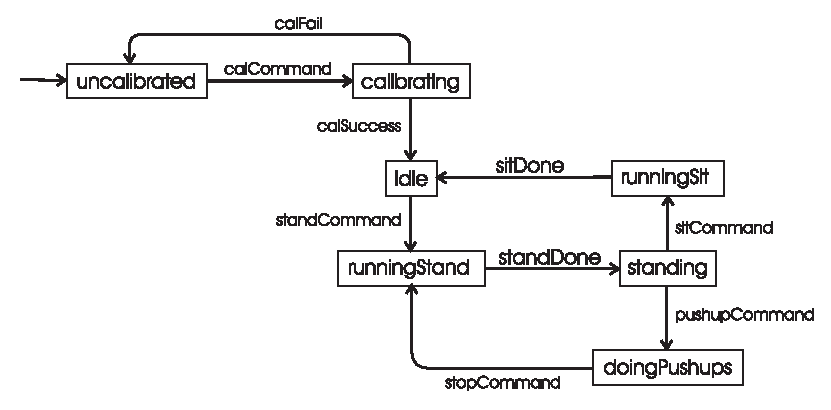
\epsfig{file=sup.eps}
\caption{A state machine, called {\tt Supervisor}, which is implemented
in this section. This machine ``supervises'' the activity of other controllers,
including other state machines. The events are either command events (which
check the remote control state) or time events. Based on the remote control
activity, the machine calibrates, stands, sits or does ``pushups''.
\label{fig-supervisor}
}\end{center}
\end{figure}

The transition table that corresponds to Figure \ref{fig-supervisor}, and which
should be saved in a file called {\tt Supervisor.dsc} is as follows:

\begin{codesegment}
  Transition uncalibrated calCommand calibrating
  Transition calibrating calFail uncalibrated
  Transition calibrating calSuccess idle
  Transition idle standCommand runningStand
  Transition runningStand standDone standing
  Transition standing sitCommand runningSit
  Transition runningSit sitDone idle
  Transition standing pushupCommand doingPushups
  Transition doingPushups stopCommand runningStand
  Initial uncalibrated
\end{codesegment}

There are seven states. {\tt uncalibrated} is the initial state, corresponding
to the situation that the robot has just been turned on. {\tt calibrating} is
the state the robot will be in while running a calibration state machine for
each leg. In the {\tt idle} state, the robot will be sitting with its motor
drives deactivated to save power. In the {\tt runningStand} state, the robot
will be running the {\tt standMachine} state machine which brings the robot to a
standing position. In {\tt standing} state, the robot will have completed the
{\tt standMachine} and will be waiting to either sit or start doing pushups. In
the state {\tt doingPushups}, the robot will be running the {\tt
pushupController} from Section \ref{sec-pushup}. Finally, in {\tt runningSit},
the robot will be running the {\tt SitMachine} controller.

There are five ``command'' events which will correspond to remote control
events. First, the {\tt calCommand::check()} method, which signals the user's intention
to calibrate the robot's legs, will be true when the left joystick is pushed
forward. The {\tt standCommand::check()} method, which signals the user's
intention to stand the robot up from idle mode, will be true when the left
joystick is pushed backward. The {\tt pushupCommand::check()} method, which
signals the user's intention to start the pushup controller from standing mode,
will be true when the left joystick is pushed forward. The {\tt
stopCommand::check()} method, which signals the user's intention to stop the
pushup controller, will be true when the left joystick is pushed backward. The
{\tt sitCommand::check()} method, which signals the user's intention to make the
robot sit when in standing mode, will be true when the left joystick is pushed
to the left.

The other events, {\tt calibSuccess}, {\tt calibFail}, {\tt standDone} and {\tt
sitDone}, correspond to the various controllers coming to completion. For
example, when the {\tt StandMachine} has finished, its {\tt isDone()} flag
returns true. Thus, {\tt standDone::check()} calls this method. As the figure
shows, while each of the controllers is running, the {\tt Supervisor} will be in
a mode that is waiting for a signal that the controller has completed, before
moving on to a state that waits for the next user input. The exception is the
{\tt doingPushups} state, which is terminated upon a remote control action from
the user.

\subsubsection{Coding the Supervisor}

We will see that there are very few things to be done to code up this seemingly
complex state machine. First, we use {\tt sm-setup.pl} to create skeleton header
and code files from the {\tt Supervisor.dsc} file. This creates 90\% of the code
for the {\tt Supervisor} machine.

The header, {\tt Supervisor.hh}, is practially finished. We just need to include
certain header files from RHexLib which define the other machines to be used and
add variables to the Supervisor class to point to the modules it will need. We
also suppose that {\tt PushupController.hh} has been created and placed in the
same directory as the supervisor code. The resulting header file is as follows:

\begin{codesegment}
#ifndef _SUPERVISOR_HH
#define _SUPERVISOR_HH

#include "ModuleManager.hh"
#include "StateMachine.hh"

// The next six includes have been added to the basic
// file produced by sm-setup.pl
#include "StdModules.hh"
#include "StandMachine.hh"
#include "SitMachine.hh"
#include "CalibMachine.hh"
#include "RemoteControl.hh"
#include "PushupController.hh"

class Supervisor : public StateMachine {

  public:

    Supervisor ( void );
    ~Supervisor ( void );
    void init ( void );
    void activate ( void );
    void deactivate ( void );

  private:

    // events
    EventObject ( CalCommand ) * calCommand;
    EventObject ( CalFail ) * calFail;
    EventObject ( CalSuccess ) * calSuccess;
    EventObject ( StandCommand ) * standCommand;
    EventObject ( StandDone ) * standDone;
    EventObject ( SitCommand ) * sitCommand;
    EventObject ( SitDone ) * sitDone;
    EventObject ( PushupCommand ) * pushupCommand;
    EventObject ( StopCommand ) * stopCommand;

    // states
    StateObject ( Uncalibrated ) * uncalibrated;
    StateObject ( Calibrating ) * calibrating;
    StateObject ( Idle ) * idle;
    StateObject ( RunningStand ) * runningStand;
    StateObject ( Standing ) * standing;
    StateObject ( RunningSit ) * runningSit;
    StateObject ( DoingPushups ) * doingPushups;

    // These six pointers have been added to the basic file produced
    // by sm-setup.pl. They will point to other modules used by the Supervisor
    PushupController * puControl;
    StandMachine     * standMach;
    SitMachine       * sitMach;
    CalibMachine     * cm[6];
    Hardware         * hw;
    RemoteControl    * rc;

};

#endif
\end{codesegment}

The next step is top modify the code file, {\tt Supervisor.cc}, produced by
{\tt sm-setup.pl}. We will do this in several steps:
\begin{enumerate}
\item Modify {\tt Supervisor::activate()} to search for the required modules
(for standing, sitting, etc.) and set up the module pointers that we added to
{\tt Supervisor.hh}.
\item Modify {\tt Supervisor::activate()} and {\tt Supervisor::deactivate()} to
grab and release the remote control module.
\item Modify the event {\tt check()} methods to check for remote control events
and controller {\tt isDone()} events.
\item Modify the state {\tt entry()}, {\tt during()} and {\tt exit()} methods
(not all of them) so that they activate and deactivate the various modules
responsible for calibrating, standing, sitting and doing pushups.
\end{enumerate}

\noindent First we modify the {\tt init()} method to search for the required modules. We
also setup the {\tt hw} pointer to point to the currently instantiated hardware
object. This is needed to enable and turn off the motor drives. The {\tt init()}
method is then:

\begin{codesegment}
void Supervisor::init ( void ) {

  int i;

  // this is where to search for the needed modules and set up pointers to them

  if ( ( standMach = ( StandMachine * ) 
         MMFindModule( STANDMACHINE_NAME, 0 )) == NULL)
     MMFatalError ( "Supervisor::init", "Cannot find Stand Machine" );
  
  if ( ( sitMach = ( SitMachine * ) 
         MMFindModule( SITMACHINE_NAME, 0 )) == NULL)
     MMFatalError ( "Supervisor::init", "Cannot find Sit Machine" );
  
  if ( ( rc = ( RemoteControl * ) 
         MMFindModule( REMOTECONTROL_NAME, 0 )) == NULL)
     MMFatalError ( "Supervisor::init", "Cannot find Remote Control" );

  if ( ( puControl = ( PushupController * ) 
         MMFindModule( "pushupcontroller", 0 )) == NULL)
     MMFatalError ( "Supervisor::init", "Cannot find Push Up Controller" );

  for ( i = 0; i < 6; i++ )
    if ( ( cm[ i ] = ( CalibMachine * ) 
           MMFindModule( CALIBMACHINE_NAME, i )) == NULL)
      MMFatalError ( "Supervisor::init", "Cannot find Calibration Machine" );

  hw = MMGetHardware();

  StateMachine::init();

}
\end{codesegment}

\noindent Next, we modify the {\tt activate()} and {\tt deactivate()} methods so
that they grab, configure and release the remote control module. The arguments
to {\tt rc->configure} are the delays of the right and left joystick inputs. A
deley of 0.005$s$, for example, means that the value has to be stable for 0.005
seconds before it is reported. The {\tt rc->setThreshold} method sets the value
above which the joystick is considered to be pushed in a particular
direction. In the {\tt deactivate()} method, we also check to see if any of the
modules that the {\tt Supervisor()} uses are active, and if they are, we
deactivate them.

\begin{codesegment}
void Supervisor::activate ( void ) {

  // Configure the RC sticks
  rc->configure ( 0.005, 0.3 );
  rc->setThreshold ( 0.5 );

  // Grab and activate the remote control interface
  MMGrabModule( rc, this );

}

void Supervisor::deactivate ( void ) {

  // Release the previously grabbed modules
  MMReleaseModule( rc, this );

  if ( standMach->getState() == MODULE_ACTIVE ) MMReleaseModule ( standMach, this );
  if ( sitMach->getState() == MODULE_ACTIVE ) MMReleaseModule ( sitMach, this );
  if ( puControl->getState() == MODULE_ACTIVE ) MMReleaseModule ( puControl, this );

  for ( i=0; i<6; i++ )
    if ( cm[i]->getState() == MODULE_ACTIVE ) MMReleaseModule ( cm[i], this );

  StateMachine::deactivate();

}
\end{codesegment}

\subsubsection{The Event {\tt check()} Methods}

Next, we add meaning to the event {\tt check()} methods. We start with {\tt
calibCommand}. This amounts to checking the value returned by the {\tt
rc->leftSick} and {\tt rc->rightStick} methods. The values returned by these
methods correspond to the cardinal map directions (north, west, northwest, etc.)
Thus, the {\tt calibCommand::check()} method below returns true if the left
joystick is pushed directly forward.

\begin{codesegment}
bool Supervisor::CalCommand::check ( void ) { 

  // Left RC stick pushed forward
 return bool ( OWNER->rc->leftStick() == RemoteControl::NORTH );

}
\end{codesegment}

\noindent The next two events check for either the sucessful completion of all the
calibration machines (one for each leg) or the unsucessful completion of at
least one of them. {\tt CalibMachine::getStatus} returns {\tt
CalibMachine::FAILURE} in the case that calibration failed, {\tt
CalibMachine::CALIBRATING} if calibration is still underway and {\tt
CalibMachine::SUCCESS} if calibration suceeded.

\begin{codesegment}
bool Supervisor::CalFail::check ( void ) {

  int i;

  // return true if any motor reports failure
  for ( i = 0; i < 6; i++ )
    if ( OWNER->cm[i]->getStatus() == CalibMachine::CALIBRATING ) return false;
  for ( i = 0; i < 6; i++ )
    if ( OWNER->cm[i]->getStatus() == CalibMachine::FAILURE ) return true;
  
  return false;

}

bool Supervisor::CalSuccess::check ( void ) {

  // return true if all motors report success
  int i;

  for ( i = 0; i < 6; i++ )
    if ( OWNER->cm[i]->getStatus() != CalibMachine::SUCCESS ) return false;
  
  return true;

}
\end{codesegment}

\noindent The stand command is issued by pushing the left joystick directly backward.

\begin{codesegment}
bool Supervisor::StandCommand::check ( void ) { 

  // Left RC stick pushed back
  return bool ( OWNER->rc->leftStick() == RemoteControl::SOUTH );

}
\end{codesegment}

\noindent Via the public interface to {\tt StandMachine}, other modules can
perceive two states. Either the machine is in the midst of standing, in which
case {\tt StandMachine::isDone()} returns {\tt false} or the machine is
completed its task and is holding steady, and {\tt isDone()} returns {\tt true}.

\begin{codesegment}
bool Supervisor::StandDone::check ( void ) { 

  return OWNER->standMach->isDone();

}
\end{codesegment}

\noindent To sit, push the left joystick directly to the left.

\begin{codesegment}
bool Supervisor::SitCommand::check ( void ) {

  // Left RC stick pushed left
  return bool ( OWNER->rc->leftStick() == RemoteControl::WEST );

}
\end{codesegment}

\noindent The {\tt SitMachine} interface is similar to the {\tt StandMachine} interface.

\begin{codesegment}
bool Supervisor::SitDone::check ( void ) {

  return OWNER->sitMach->isDone();

}
\end{codesegment}

\noindent To start doing pushups, push the joystick directly forward while in standing mode.

\begin{codesegment}
bool Supervisor::PushupCommand::check ( void ) {

  // Left RC stick pushed forward
  return bool ( OWNER->rc->leftStick() == RemoteControl::NORTH );

}
\end{codesegment}

\noindent To stop doing pushups, push the left joystick directly backward.

\begin{codesegment}
bool Supervisor::StopCommand::check ( void ) {

  // Left RC stick pushed back
  return bool ( OWNER->rc->leftStick() == RemoteControl::SOUTH );

}
\end{codesegment}

\subsubsection{The State Methods}

The next and final step is to modify the state methods. Note that we do not
modify them all as they are not all needed. For example, none of the {\tt
during()} methods are changed at all as will often be the case in supervisor
state machines. To see how the {\tt during()} methods are used, see the code of,
for example, {\tt StandMachine}. Here, only {\tt some} of the {\tt entry()} and
{\tt exit()} methods are actually required. Mostly what they do is activate and
deactivate other modules. Activation of a module is done with the {\tt
MMGrabModule} function. Deactivate is done with the {\tt MMReleaseModule()}
function.

There are six caibration machines to be activated upon entry into the {\tt
calibrating} state as follows. This method also sets the calibration method of
each machine to {\tt GROUND} which makes the robot's legs spin until the meet
with some resistance (persumably the ground).

\begin{codesegment}
void Supervisor::Calibrating::entry ( void ) {

  int i;

  for ( i = 0; i < 6; i++ ) {

    OWNER->cm[i]->setMode( CalibMachine::GROUND );
    MMGrabModule ( OWNER->cm[i], owner );

  }
}
\end{codesegment}

\noindent Upon completion of the {\tt calibrating} state, when either {\tt calibSucess}
or {\tt calibFail} become active, we release the calibration machines, thereby
deactivating them.

\begin{codesegment}
void Supervisor::Calibrating::exit ( void ) {

  int i;

  for ( i = 0; i < 6; i++ )
    MMReleaseModule ( OWNER->cm[i], owner );
}
\end{codesegment}

\noindent Successful calibration leaves the robot calibrated with the motor
drives off. Thus, to start standing, we need to enable the motor drives and
then grab the stand machine.

\begin{codesegment}
void Supervisor::RunningStand::entry ( void ) {

  int i;

  for ( i = 0; i < 6; i++ )  // enable motor drives
    OWNER->hw->driveEnable( i, true );
  
  MMGrabModule ( OWNER->standMach, owner );
}
\end{codesegment}

\noindent We leave the standing machine running during the {\tt standing}
state though it is in the standing position. This is because the {\tt
StandMachine} holds the robot in the upright position after it is done. We
release (and deactivate) the standing machine only when leaving the {\tt
standing} state on our way either to sitting or doing pushups.

\begin{codesegment}
void Supervisor::Standing::exit ( void ) {

  MMReleaseModule ( OWNER->standMach, owner );

}
\end{codesegment}

\noindent To start sitting, we grab the sit machine (don't let anyone just anyone grab
your sit machine!).

\begin{codesegment}
void Supervisor::RunningSit::entry ( void ) {  

  MMGrabModule ( OWNER->sitMach, owner );

}
\end{codesegment}

\noindent When the {\tt SitMachine} is done, we release it and also disable
the motor drives to save power.

\begin{codesegment}
void Supervisor::RunningSit::exit ( void ) {

  int i;

  for ( i = 0; i < 6; i++ )  // disable motor drives
    OWNER->hw->driveEnable( i, false );

  MMReleaseModule ( OWNER->sitMach, owner );
}
\end{codesegment}

\noindent Finally, it is easy to incoorporate the pushup controller, we just grab and
release it as needed:

\begin{codesegment}
void Supervisor::DoingPushups::entry ( void ) {

  MMGrabModule ( OWNER->puControl, owner );

}

void Supervisor::DoingPushups::exit ( void ) {

  MMReleaseModule ( OWNER->puControl, owner );

}
\end{codesegment}

\subsubsection{A {\tt main()} File}

One more piece is required to get the {\tt Supervisor} runnning. We need a main
file. The following will do.

\begin{codesegment}
#include <stdio.h>
#ifdef _QNX4_
#include <sys/sched.h>
#include <unistd.h>
#endif
#include "sysutil.hh"
#include "ModuleManager.hh"
#include "StdModules.hh"
#include "StateMachine.hh"
#include "Supervisor.hh"
#include "RemoteControl.hh"
#include "PushupController.hh"
#include "MichiganHW.hh"

MichiganHW hw;

class UserModule : public Module {

  public:

    UserModule ( void ) : Module( "userinput", 0, false, false ) { };

    void  init ( void ) {}
    void  uninit ( void ) {}
    void  activate ( void ) {}
    void  deactivate ( void ) {}
    void  update ( void ) {

      int i;

      if ( kbhit() ) {

        // Diable all motor drives
        for ( i = 0 ; i < 6 ; i++) 
          hw.driveEnable ( i, false );

        MMShutdown();
        MMPowerOff( );

      }
    }
} umod;

int main ( void ) {

#ifdef _QNX4_
  setprio( getpid(), 23 );
#endif

  MMReadConfigFile( "rhex_michigan.rc" );

  // Read the application dependent configuration file
  MMReadConfigFile( "sup.rc" );

  MMChooseHardware ( & hw );

  Supervisor supervisor;
  PushupController puc;

  // Create and add all the standard modules
  RHexAddStdModules();

  // Add the user module, pushup controller and supervisor
  MMAddModule ( &umod, 1, 0, USER_CONTROLERS );
  MMAddModule ( &puc, 1, 0, USER_CONTROLLERS );
  MMAddModule ( &supervisor, 1, 0, USER_CONTROLLERS );

  // Activate the supervisor modules
  MMActivateModule ( &supervisor );

  MMMainLoop();
  MMShutdown();
  return 0;

}
\end{codesegment}

The machines for calibration, standing and sitting as well as the
remote control module are all added to the Module Manager by the command {\tt
RHexAddStdModules()}. Only the {\tt Supervisor} and the {\tt PushupController}
are added in {\tt main()}. Also, only the {\tt Supervisor} module is activated
in {\tt main()}. It takes care of activating everything else it needs. We have
also added a simple module, called {\tt UserModule}, which allows the user to
stop the program by pressing any key.

Note, we have
chosen to configure this program to use the {\tt Michigan.hh} hardware library
and the {\tt rhex\_michigan.rc} file.

\section{Hardware Components}

This section gives a tutorial on how to deal with Hardware interfaces in
RHexLib. The following sections briefly explain and give examples on how to
accomplish increasingly complex tasks related to RHexLib's low level
hardware interface.

Section \ref{sec:using_hardware} outlines how to use one of the existing
Hardware components. Section \ref{sec:unsupported_hardware} explains how to
access a piece of hardware currently unsupported by the interface. Section
\ref{sec:adding_hardware} presents how to augment the Hardware class
interface with a new type of component, which is general and useful enough
to be implemented by all versions of the hardware. Finally, Section
\ref{sec:new_hardware_class} outlines how to create a completely new
hardware library, conforming to the interface of the Hardware class whose
implementation is different from the existing hardware libraries.

\subsection{Using the Hardware Class Interface}
\label{sec:using_hardware}

RHexLib solves the issue of being able to use the same higher level control
code with different versions of the underlying low level hardware (such as
encoders, analog IO, digital IO etc.) by the use of {\em hardware
libraries}, instantiating specific implementations of the {\tt Hardware}
class and the associated component classes. The abstract base templates for
these classes are defined in {\tt Hardware.hh} and their class interfaces
are explained in detail in Chapter \ref{sec:hardware_interface}.

As a consequence, the first thing that any RHexLib program does is to create
an instance of the desired hardware class, which are always inherited from
the abstract base class {\tt Hardware}. Currently, RHexLib distribution
defines {\tt MichiganHW}, {\tt McGillHW}, {\tt SimSectHW} and {\tt
  VirtualHW}, supporting the Michigan RHex, McGill RHex, SimSect simulation
interface and a simple simulator for free running motors,
respectively. Usually, the hardware object is created as a global object
(whose constructor is called before main() is executed) in one of the source
files.

\begin{codesegment}
#include "SimSectHW.hh"
SimSectHW hw;
\end{codesegment}

The next thing that needs to be done is to inform the module manager about
the newly created hardware object, making it possible for all modules and
components in the system to get their hands on this object for low level
hardware access. This is accomplished with the {\tt MMChooseHardware()}
function, which calls the appropriate initialization methods of the hardware
object. Usually, this function is called {\em after} loading the
configuration symbol table because often, the initialization of the hardware
accesses the configuration symbols.

\begin{codesegment}
int main( int argc, char **argv ) {

  MMReadConfigFile( "rhex_standard.rc" );
  MMChooseHardware( &hw );

  // the rest of main() code goes here...

  MMMainLoop(); // Invoke the main module manager loop
}
\end{codesegment}

Once these steps are completed, then all the modules and components in the
system can access low level hardware functionality through this
object. However, due to the data abstraction principles, module
implementations must {\em never} rely on the presence of a global module
object. Different programs might instantiate this object with different
names, or maybe even not as a global variable. Therefore, the {\tt
  MMGetHardware()} function is provided to acquire a pointer to the current
hardware object through the module manager's central database. Usually,
modules acquire this pointer in their {\tt init()} methods and store it
locally.

\begin{codesegment}
void DummyModule::init( void ) {

  local_hw_ptr = MMGetHardware();

  // Rest of the init() code...
}
\end{codesegment}

The Hardware class itself provides a few methods to access some general
hardware facilities such as reading the clock, enabling/disabling motor
drives ({\em *TODO*: This should probably be part of DCMotorHW instead of
  the Hardware class}) etc. The details of these methdos are explained in
Section \ref{sec:hardware_class}.

In contrast, the functionality related to individual hardware components are
accessed through component class interfaces. The Hardware class holds
pointers to instances of these interfaces, through which modules can get
access to component specific functionality. For example, 

\begin{codesegment}
  uint16 count = local_hw_ptr->encoders->read( 3 );
\end{codesegment}

\noindent would read the 16 bit encoder count for the third axis. Current,
the Hardware class has pointers to a few standard component types, all of
which are explained in detail in Chapter \ref{sec:hardware_interface}.

\begin{classdef}
class Hardware {
public:

  // Some other stuff...

  EncoderHW   * encoders;
  AnalogHW    * analogIO;
  DigitalHW   * digitalIO;
  TimerHW     * timers;
  AccelHW     * accels;
  GyroHW      * gyros;
  PowerHW     * power;
  SwitchHW    * switches;
  DialHW      * dials;
  DCMotorHW   * dcmotors;
};
\end{classdef}

One {\em very important} feature to note is that, these fields are
initialized to {\tt NULL} if the particular hardware implementation does not
support the corresponding component. As a consequence, it is {\tt always} a
good idea for a module to check the presence of a desired hardware component
in the init function, and exit with a fatal error if it does not exist.

\begin{codesegment}
void DummyModule::init( void ) {

  local_hw_ptr = MMGetHardware();

  if ( local_hw_ptr->encoders == NULL )
    MMFatalError( "DummyModule::init", 
                  "Encoder Hardware component not supported!" );

  if ( local_hw_ptr->analogIO == NULL )
    MMFatalError( "DummyModule::init", 
                  "Analog I/O Hardware component not supported!" );

  // Rest of the init() code...
}
\end{codesegment}

Note that this kind of error checking does not introduce any runtime
inefficiency because it is done only once when the module is added through
{\tt MMAddModule()}.

\subsection{Accessing an Unsupported Piece of Hardware}
\label{sec:unsupported_hardware}

Suppose you wanted to quickly add a sensor or actuator, which is not
included in the set of standard components of Chapter
\ref{sec:hardware_interface}. This section explains how this can easily be
done.

Obviously, augmenting the Hardware interface by adding another component
seems to be the natural solution. However, this is relatively time consuming
and involves modifying the core library distribution, which should be
avoided for prototyping purposes. Section \ref{sec:adding_hardware} explains
how this can be done in cases where the component in question is {\em
extremely} useful and you believe that it should definitely be part of the
standard set of components. However, even then, testing the component and
its interface through the methods described in this section is the best
first solution.

In this context, there are two scenarios, which call for two different
solutions. If the sensor in question only requires a few I/O instructions
(possibly using the existing hardware components such as the analog I/O) and
no significant processing, then you need to write a simple non-module class
to encapsulate the interface. For example, for a range sensor which is
connected to the analog inputs and only requiring a simple affine mapping to
obtain the range data, you could create a class {\tt RangeSensor}.

\begin{classdef}
class RangeSensor {
  public :

    RangeSensor( uint analog_channel ) { 

      local_hw_ptr = MMGetHardware();

      if ( ( local_analogio_ptr = local_hw_ptr->analogIO ) == NULL )
        MMFatalError( "RangeSensor::RangeSensor",
                      "Analog I/O hardware component does not exist" );
      channel = analog_channel; 
    };
  
    float read( void ) { 
      return analog_to_range( local_analogio_ptr->read( channel ) );
    };

  private:

    float analog_to_range( float analog_value );

    Hardware *local_hw_ptr;
    AnalogIO *local_analogio_ptr;
    uint     channel;
};
\end{classdef}

From this point on, anybody who wants to use the range sensor would create
an instance of this class and access the range value through {\tt
  RangeSensor::read()} method. Note that the {\tt analog\_to\_range()} method
is where the conversion to the range value is performed. If you think this
much code is unnecessary and want to do it the dirty way, you could simply
write a global {\tt AnalogToRange()} function and use it on a direct reading
from the analog inputs.

There may be cases, however, where the processing required to perform the
conversion is too long and should be performed only once per cycle for
efficiency purposes. It might also be the case that the sensor's output is
based on a time history of a data stream, such as a filtered sensor. In
those cases, such a simple class interface will not be sufficient and you
will need to create a {\em Module}.

Defining such a module will make it possible to do processing only once per
cycle in the module's update function, and provide access to the hardware
component's functionality through local interface methods. In the rest of
this section, we will work out an example of such a module, implementing a
simple filtered version of the above range sensor.

\begin{classdef}
class RangeSensorModule : public Module {
  public:

    RangeSensorModule::RangeSensorModule( uint analog_channel );

    float read( void ) { return range; };

    void init( void ) { };
    void uninit( void ) { };
    void activate( void );
    void deactivate( void ) { };
    void update( void );

  private:

    float analog_to_range( float analog_value );

    float range;
};
\end{classdef}

The module's update function will handle reading the analog input, filtering
and storing the latest filtered value in the private member {\tt
  range}. Also, we need to implement the {\tt activate()} function to reset
the internal filter state.

The module constructor is very similar to the RangeSensor class. One small
difference is that, we use the module {\em index} to store the analog
channel number in this case. This is accomplished by creating the base
Module class with name {\tt "rangesensor"}, the index corresponding to the
analog channel as a multi-user, non-polling module. A consequence of this is
that, you will be able to create only one {\tt RangeSensorModule} module for
a particular analog input channel because two modules with the same name and
index cannot coexist in the module manager.

\begin{codesegment}
RangeSensorModule::RangeSensorModule( uint analog_channel )
  : Module( "rangesensor", analog_channel, false, false ) {

  local_hw_ptr = MMGetHardware();

  if ( ( local_analogio_ptr = local_hw_ptr->analogIO ) == NULL )
    MMFatalError( "RangeSensorModule::RangeSensorModule",
                  "Analog I/O hardware component does not exist" );
};
\end{codesegment}

The activate function is very simple and simply resets the range value to
its initial value. Note the use of the {\tt getIndex()} method from the base
Module class to obtain the analog channel number.

\begin{codesegment}
void RangeSensorModule::activate( void ) {

  range = analog_to_range( local_analogio_ptr->getIndex() );
};
\end{codesegment}

Finally, the bulk of the work is done in the update method. We use an
exponantial filter, which computes the range as a weighted sum of the
previous range value and the current raw range reading from the analog
channel. We used hard-coded weight values, although these values could
easily be configurable through some module methods or configuration
variables.

\begin{codesegment}
void RangeSensorModule::update( void ) {

  float unfiltered_range;

  unfiltered_range = analog_to_range( local_analogio_ptr->getIndex() );

  range = 0.9 * range + 0.1 * unfiltered_range;
};
\end{codesegment}

This implementation is very efficient because it only reads the analog input
and filters the signal once per cycle. Even if the range value is read 100
times per cycle, it is computed only once.

\subsection{Adding a Component to the Hardware Class Interface}
\label{sec:adding_hardware}

So, if you are reading this section, it means that you have decided the
hardware component that you want to add is generic enough that it deserves
to be in the standard set of hardware components. Even though the
modifications necessary to accomplish this are minimal and will have no
effect on the rest of the system, there are a couple of issues to be
considered before you plunge ahead.

\begin{itemize}
\item{In RHexLib, the hardware layer is designed to capture the {\em
minimal} functionality regarding low level hardware access, which is
platform dependent. It is {\em extremely} important to limit the scope of
the component that you want to add to the smallest possible set of
functionality which you think will be different for different versions of
the robot or the simulation. In most of the cases, it should simply deal
with raw data acquisition and possibly some basic unit
conversions. Everything else should be implemented separately, either as
modules or classes. This makes it possible to reuse all the hardware
independent code for all hardware versions.

For example, in defining the {\tt GyroHW} class, we did not put the
procedures for integrating the angular velocities or estimating body state
below the hardware layer. Instead, the only hardware dependent
functionality, which is the acquision of the angular rate information from
the physical (or simulated) hardware is implemented through {\tt GyroHW}
interface. The rest of the functionality is independent of which hardware is
used, and can be implemented in the form of commonly usable modules.}
\item{Everybody who will use the library in the future will be forced to use
the new component interface that you are about to design. Consequently, it
is extremely important that all current developers of the library (at least
the core set of people) should have a chance to comment on the interface you
propose. Before starting any implementation, you should collect these
opinions.}
\end{itemize}

Having considered these issues, the first step is to define the interface of
the hardware component. As an example, we will design an LCD text/graphics
display interface component, {\tt LCDisplayHW}.

Following the above guidelines, we would like this interface to be as
general as possible, while limiting its scope to only hardware dependent
functionality. We would like the interface to support both text and graphics
modes in black and white, as well as a way to figure out which modes are
possible in a particular instantiation. While in text mode, the basic
operation is to put an ASCII character on a given coordinate. 

In contrast, the graphics mode requires the ability to modify individual
pixels, as well as pasting a rectangular graphics object to a given location
on the display. Other methods such as drawing rectangles, lines circles
etc. would have been possible, but we leave those out for simplicity.

The following class definition outlines the interface we propose. This
definition should go in {\tt Hardware.hh}, before the {\tt Hardware} class
definition. 

\begin{classdef}
class LCDisplayHW {
  public:
    virtual ~LCDisplayHW( ) { };

    typedef enum { TEXT_MODE = 0x01, GRAPHICS_MODE = 0x02 } DisplayMode;

    virtual bool        setMode ( DisplayMode newMode ) = 0;
    virtual DisplayMode getMode ( void ) = 0;

    virtual void clearDisplay ( void ) = 0;
    virtual void getDisplaySize ( int *width, int *height ) = 0;

    virtual bool writeChar ( uint x, uint y, char c ) = 0;
    virtual char readChar ( uint x, uint y ) = 0;

    virtual bool getPixel ( uint x, uint y ) = 0;
    virtual bool setPixel ( uint x, uint y, bool val ) = 0;
    virtual bool pasteBitmap ( uint x, uint y, 
                               uint width, uint height, char *bitmap ) = 0;
};
\end{classdef}

Note that all the methods are defined as pure virtual functions because the
real work will be done in classes inherited from {\tt LCDisplayHW} in
specific hardware libraries. We will not give the details of what each of
these methods are supposed to do as it is pretty obvious from their names
and arguments. This collection of methods covers quite a large number of
display types and is an appropriate start for the desired functionality. We
kept this example simple for documentation purposes, but the interface
certainly could be augmented to handle more complicated features.

Having decided on the component interface and defined the component class
{\tt LCDisplayHW}, the next step is to change the {\tt Hardware} class to
support the new component. Two modifications are needed: Adding a pointer to
an instance of the new component to the Hardware class public members, and
changing the Hardware class constructor to initialize this pointer to {\tt
NULL}.

\begin{classdef}
class Hardware {
public:

  Hardware( void ) { 
    lcdisplay = NULL;      // <<<<< New addition.
    encoders = NULL; 
    analogIO = NULL; 

    // ( Some other NULL assignments which were already there... )

  };

  // ( Some unrelated method declarations ... )

  LCDisplayHW * lcdisplay; // <<<<< New addition.
  EncoderHW   * encoders;

  // (Some other pointers which were already there ... )

};
\end{classdef}

These are all the modifications needed to the core library. The remaining
steps involve the actual implementation in a specific hardware library. Note
that initially, you will only need to change the hardware library that you
will immediately be working with. {\em You do not need to change any other
library as this point}. The member variable {\tt lcdisplay} will by default
be {\tt NULL}, which means that this component will simply be unsupported by
the other existing libraries. Any module that follows the guidelines of
Section \ref{sec:using_hardware} will notice this in their {\tt init()}
function and give a fatal error in the presence of a library which does not
support this component.

The final steps hence involve augmenting your current hardware library with
a specific implementation of this component. For this example, we will
change {\tt MichigahHW} class.

First, we define a new class, inherited from {\tt LCDisplayHW}, where all
the real work will be done. The following code would go into {\tt
  UMichHW.hh} in {\tt hardware/UofM/UMichLCD.hh} and is internal to the
hardware library and will not be visible to any user of RHexLib.

\begin{classdef}
class UMichLCD : LCDisplayHW {
  public:
    UMichLCD( void )
    ~UMichLCD();

    bool        setMode ( DisplayMode newMode );
    DisplayMode getMode ( void );

    void clearDisplay ( void );
    void getDisplaySize ( int *width, int *height );

    bool writeChar ( uint x, uint y, char c );
    char readChar ( uint x, uint y );

    bool getPixel ( uint x, uint y );
    bool setPixel ( uint x, uint y, bool val );
    bool pasteBitmap ( uint x, uint y, 
                       uint width, uint height, char *bitmap );
};
\end{classdef}

Note that all the pure virtual functions of the base class are implemented
by this new class. We will not give the code for these methods, but remember
that these methods will be where all the hardware access, buffering, low
level I/O etc. are done. Usually, it a good idea to create separate files
for the implementations of each hardware component.

Now to the final step. The {\tt MichiganHW} class is inherited from the base
{\tt Hardware} class and is responsible from filling in the component
pointers for the pieces of hardware that it supports. As a consequence, we
now need to go in {\tt hardware/UofM/MichiganHW.cc} and change the method
{\tt MichiganHW::initialize()} to create an instance of {\tt UMichLCD} and
initialize the corresponding component pointer.

\begin{codesegment}
void MichiganHW::initialize( void ) {

  // ( Some unrelated initialization code ... )

  lcdisplay = new UMichLCD;        // <<<<< New addition.
  encoders = new MEncoder;
  // ( Initialization of other pointers ... )

  // ( Some other unrelated initialization code ... )
}
\end{codesegment}

Similarly, you will need to change the method {\tt MichiganHW::cleanup()} to
delete the created component object.

\begin{codesegment}
void MichiganHW::cleanup( void ) {

  // ( Some unrelated cleanup code ... )

  if ( lcdisplay != NULL ) delete lcdisplay;        // <<<<< New addition.
  if ( encoders != NULL ) delete encoders;
  // ( Cleanup of other pointers ... )

  // ( Some other unrelated cleanup code ... )
}
\end{codesegment}

This completes the necessary changes to access your new LCD through its
uniform class interface. Maintainers of other hardware libraries can augment
their own implementations to support their particular LCD hardware, at which
point they will be able to use all of you higher level modules accessing the
LCD component. 

\subsection{Creating a New Hardware Class}
\label{sec:new_hardware_class}

When a new major hardware revision is made, or when RHexLib is being ported
to a completely different platform, a new hardware library will need to be
created. Even though all of the principles and methods explained in previous
sections will still apply, creating a new hardware library is somewhat more
complicated and involves a lot more coding. Before proceeding, please read
Chapter \ref{sec:hardware_interface} for the details of the Hardware class
and the supported hardware components.

The first step is to decide on a name for the new Hardware class to be
created. The name should be sufficiently descriptive, keeping in mind that
there may be later hardware libraries with similar names. Even though it is
possible to use an existing Hardware class name, keeping different
implementations in different directories and libraries, it is better to have
different class names as it will avoid later confusion.

In this section, we will present an example hardware class, {\tt ExampleHW},
together with how to implement the standard set of components and add the
resulting library to the distribution.

The RHexLib core distribution includes a directory, {\tt hardware}, which
contains individual directories for each of the supported hardware
libraries. Normally, the newly created library and the associated files
would go into a separate directory under {\tt hardware}. However, for
testing and debugging purposes, it is best to start in a local directory of
your own. Let's name it {\tt example} for the time being.\\

\noindent{\tt
\# cd \~{}/RHex/UlucDevel \\
\# mkdir hardware \\
\# mkdir hardware/example \\
\# cd hardware/example \\
}

The next step is to create the Makefile which will generate the library. You
can copy one from {\tt tools/Makefile.libsample} and change the lines {\tt
  LIBRARY}, {\tt SOURCES} and {\tt AUXFLAGS} as necessary. For our example,
we will name the library {\tt libexamplehw.a}. The {\tt SOURCES} line will
be completed as we add more sources. Finally, {\tt AUXFLAGS} should contain
any additional compilation flags, such as include search paths and library
search paths.

At this point, we are ready to create the main hardware header file, which
will be the only visible component of the hardware library to the users of
RHexLib. When the new library becomes part of RHexLib core distribution,
this header file will go into the {\tt include} directory, from where
anybody can include it. For now, create the file {\tt ExampleHW.hh} in your
local directory with the appropriate license headers and the following class
definition.

\begin{classdef}
#include "Hardware.hh"

class ExampleHW : public Hardware {

public:
  ExampleHW( void );
  ~ExampleHW( );

  void initialize( void );
  void cleanup( void );

  CLOCK readClock( void );
  CLOCK readUClock( void );

  void driveEnable( uint index, bool enable );
};
\end{classdef}

The implementations of these methods would go into {\tt ExampleHW.cc}. We
will describe what needs to be done in each of these e in later paragraphs.

The next step is to define implementations for each of the standard
components supported by the Hardware interface. For this purpose, you need
to create a header file {\tt ExComponents.hh}, where you define classes
derived from each of the components your hardware library will support. Note
that you do not need to support all the components, but be aware that what
you leave unsupported will prevent controllers using those components from
functioning. This header file will be local to the library and will not be
visible by the users of the library.

\begin{classdef}
#include "Hardware.hh"

class ExEncoder : public EncoderHW {
public:
  ExEncoder( void );
  ~ExEncoder( );

  void   enable( uint index );
  void   disable( uint index );
  uint16 read( uint index );
  void   reset( uint index );
};

class ExAnalog : public AnalogHW {
public:
  ExAnalog( void );
  ~ExAnalog( );

  float read( uint index );
  void  write( uint index, float value );
  void  outputRange( uint index, float *min, float *max );
  float readOutput( uint index ) { return output[index]; };
};

// Followed by definitions of other components.
\end{classdef}

You can add other private or public methods and members to these
classes. However, keep in mind that they will NOT be part of the standard
Hardware class interface and they should only be used locally by the files
in the library that we are about to create.

The next stage is where the bulk of the work is done. It involves
implementing the methods of each of these components, in a way that conforms
with the specifications of Chapter \ref{sec:hardware_interface}. The
implementation is completely up to you, although you can look at the
existing hardware libraries as examples.

Usually, there are pieces of hardware, such as PC104 cards etc. which have
functionality corresponding to more than one of these hardware
components. In that case, it is a very good idea to create a separate class
interface to access that piece of hardware, which is then used by these
component interfaces to implement specific functionality. Examples of such
classes can be found in the {\tt hardware/common} directory. The {\tt
dm6814} and {\tt mpc550} classes are designed precisely for that purpose.

At this point, we will need to go back and explain what the {\tt initialize}
and {\tt cleanup} methods of the {\tt Hardware} class are for. When a
RHexLib program calls {\tt MMChooseHardware()}, the {\tt initialize()}
method of the hardware class is called. In this method, you must do all
proper initialization of the hardware, as well as making sure that only one
instance of the same hardware object is created. The following list
summarizes what needs to be done in this method.

\begin{itemize}
\item{Check whether another instance of this hardware object was created
before. If so, give an error because only one hardware object should exist
in the system at once. You can perform this check by keeping a global flag
to keep track of creation status.}

\item{Create instances of low level hardware access classes (such as {\tt
dm6814} or {\tt mpc550}), possibly assigning them to global pointers
accessible by the component interfaces.}

\item{Create instances of all supported component interface objects and fill
in the component pointers of the {\tt Hardware} class. These pointers are
where users of RHexLib will get their hands on the hardware components.}

\item{Initialize all local member variables with proper values.}

\end{itemize}

Analogously, the {\tt cleanup()} method undoes what the {\tt initialize()}
method does, by destroying all instances of low level hardware classes and
the component interfaces. The cleanup method, through the destructors of the
components and the low level hardware classes, makes sure that the robot is
properly uninitialized before the program exits.

Most likely, the low level hardware access classes will be needed by the
component interfaces that you will implement. Hence, the {\tt initialize()}
and {\tt cleanup()} methods of the Hardware class will be among the first
things you will need to implement. You will also need to implement the other
methods of the {\tt Hardware} class, such as {\tt driveEnable()}, {\tt
readClock()}. We will not present any specific implementation of the {\tt
ExampelHW} components, but you can refer to the implementations of the
existing libraries in Chapter \ref{sec:hardware_libraries}.






%
% This file is part of RHexLib, 
%
% Copyright (c) 2001 The University of Michigan, its Regents,
% Fellows, Employees and Agents. All rights reserved, and distributed as
% free software under the following license.
% 
%  Redistribution and use in source and binary forms, with or without
% modification, are permitted provided that the following conditions are
% met:
% 
% 1) Redistributions of source code must retain the above copyright
% notice, this list of conditions, the following disclaimer and the
% file called "CREDITS" which accompanies this distribution.
% 
% 2) Redistributions in binary form must reproduce the above copyright
% notice, this list of conditions, the following disclaimer and the file
% called "CREDITS" which accompanies this distribution in the
% documentation and/or other materials provided with the distribution.
% 
% 3) Neither the name of the University of Michigan, Ann Arbor or the
% names of its contributors may be used to endorse or promote products
% derived from this software without specific prior written permission.
% 
% THIS SOFTWARE IS PROVIDED BY THE COPYRIGHT HOLDERS AND CONTRIBUTORS
% "AS IS" AND ANY EXPRESS OR IMPLIED WARRANTIES, INCLUDING, BUT NOT
% LIMITED TO, THE IMPLIED WARRANTIES OF MERCHANTABILITY AND FITNESS FOR
% A PARTICULAR PURPOSE ARE DISCLAIMED. IN NO EVENT SHALL THE REGENTS OR
% CONTRIBUTORS BE LIABLE FOR ANY DIRECT, INDIRECT, INCIDENTAL, SPECIAL,
% EXEMPLARY, OR CONSEQUENTIAL DAMAGES (INCLUDING, BUT NOT LIMITED TO,
% PROCUREMENT OF SUBSTITUTE GOODS OR SERVICES; LOSS OF USE, DATA, OR
% PROFITS; OR BUSINESS INTERRUPTION) HOWEVER CAUSED AND ON ANY THEORY OF
% LIABILITY, WHETHER IN CONTRACT, STRICT LIABILITY, OR TORT (INCLUDING
% NEGLIGENCE OR OTHERWISE) ARISING IN ANY WAY OUT OF THE USE OF THIS
% SOFTWARE, EVEN IF ADVISED OF THE POSSIBILITY OF SUCH DAMAGE.

%%%%%%%%%%%%%%%%%%%%%%%%%%%%%%%%%%%%%%%%%%%%%%%%%%%%%%%%%%%%%%%%%%%%%%
% $Id: faq.tex,v 1.5 2001/07/19 16:35:56 ulucs Exp $
%
% Created       : Uluc Saranli, 01/06/2001
% Last Modified : Uluc Saranli, 06/27/2001
%
%%%%%%%%%%%%%%%%%%%%%%%%%%%%%%%%%%%%%%%%%%%%%%%%%%%%%%%%%%%%%%%%%%%%%%

\chapter{Frequently Asked Questions}

\section{Installation}

\begin{enumerate}
\item
\end{enumerate}

\section{Makefiles and Compiling}

\begin{enumerate}
\item
\end{enumerate}

\section{Module Manager and Modules}

\begin{enumerate}
\item{In the function call {\tt MMGrabModule(moduleptr,this)}, what does the
    {\tt this} keyword do?}\par
The C++ keyword {\tt this} is a pointer to the class object for which the
currently executing method was called. In this case, it points to the
current module.

\item{What happens when I try to read more than one configuration file with
    {\tt MMReadConfigFile()}?}\par
The contents of the new configuration file are appended to the existing
symbol table. If a symbol is redefined, the new value replaces the old one.

\item{What happens if two modules have the same order value?}\par
The order in which their update functions are called in the same module
manager cycle is unspecified. It may depend on the time of the day, the
weather, barometric pressure etc. etc.
\end{enumerate}

\section{State Machines}

\begin{enumerate}
\item{Why do state machines have no {\tt update()} method?}\par

The \StateMachine\ class is derived from the \Module\ class and it defines
the update function itself. It performs various importnat tasks such as
checking the currently active events, calling the during() function of the
current state and performing state transitions as necessary.

When you need the update functionality of modules in state machines, you
should use the {\tt during()} functions of states. The during function of
the current state is called every time the state machine module itself is
updated.
\end{enumerate}

\section{Hardware Access}

\begin{enumerate}

\item{What are the resolutions of MMReadTime() and MMReadUTime()?}\par
The resolutions of both depend on the operating system as well as the
actual timer hardware on the CPU board. On QNX, {\tt MMReadTime()} has a
resolution equal to the system timer, which in RHexLib is set to 1
milliseconds. In contrast, {\tt MMReadUTime()} uses timers with the highest
available resolution. In QNX, on a 486, it has 0.2 microseconds or so
resolution whereas on a Pentium, it uses the CPU's instruction counter and
has 0.003 microseconds resolution.

\item{How do I decide when to add a new component to the Hardware class and
    what its interface should be?}\par
\end{enumerate}

\section{How do I do ...?}

\begin{enumerate}
\item
\end{enumerate}

\section{C++ Related}

The questions in this section relate to general C++ issues. A good C++ book
will always be a better reference than this section.

\begin{enumerate}
\item{Why is there no destructor for some classes?}\par
You need to define a destructor for a class, if there are explicit
deallocations or cleanup operations that you need to do. Usually, if you
have allocated any memory in the constructor, you need to deallocate them in
the destructor. For hardware related classes, the destructor usually
uninitializes the hardware and leaves it in a clean state. If you do not
need such operations, you do not need to define a destructor. Deletion of
the class object itself is done by code generated by the compiler.

\item{What is the {\tt virtual} keyword I see in some of the class
    definitions? What is the meaning of {\tt virtual mymethod( void ) = 0}?}
Virtual functions are a very useful feature of C++. They allow you to
override the method definitions of a class by its derived classes. This way,
if a derived class wants to provide a better, or more specific
implementation of a method which is already defined by its parent class,
this possible if the parent class had defined its method to be "virtual".

The {\tt = 0} at the end of a virtual method declaration defines the
function to be {\em pure virtual}. This is a special virtual function, in
that the parent class does not define what this function does {\em at
  all}. It only declares the arguments, the name, and the return value of
the method and leaves it up to its derived classes to define the
function. This is a very useful way for a class to define a {\em uniform 
  interface}, rather than an implementation. For example, the \Module\ class
has many pure virtual functions, which {\em must} be defined by all the
derived module classes, enforcing a uniform interface for all of them.

\item{What are abstract base classes?}
A class which has at least one pure virtual function as one of its methods
is an abstract base class. Instances of abstract base classes cannot be
created (i.e. the statement {\tt new Module} would fail to compile) because
some of their methods are left undefined. It is impossible to create an
object whose methods are still undefined. These classes only become useful
when you derive a class from them. That is why they are called (abstract)
base classes.
\end{enumerate}

\section{Common Pitfalls}

\begin{enumerate}
\item
\end{enumerate}



%
% This file is part of RHexLib, 
%
% Copyright (c) 2001 The University of Michigan, its Regents,
% Fellows, Employees and Agents. All rights reserved, and distributed as
% free software under the following license.
% 
%  Redistribution and use in source and binary forms, with or without
% modification, are permitted provided that the following conditions are
% met:
% 
% 1) Redistributions of source code must retain the above copyright
% notice, this list of conditions, the following disclaimer and the
% file called "CREDITS" which accompanies this distribution.
% 
% 2) Redistributions in binary form must reproduce the above copyright
% notice, this list of conditions, the following disclaimer and the file
% called "CREDITS" which accompanies this distribution in the
% documentation and/or other materials provided with the distribution.
% 
% 3) Neither the name of the University of Michigan, Ann Arbor or the
% names of its contributors may be used to endorse or promote products
% derived from this software without specific prior written permission.
% 
% THIS SOFTWARE IS PROVIDED BY THE COPYRIGHT HOLDERS AND CONTRIBUTORS
% "AS IS" AND ANY EXPRESS OR IMPLIED WARRANTIES, INCLUDING, BUT NOT
% LIMITED TO, THE IMPLIED WARRANTIES OF MERCHANTABILITY AND FITNESS FOR
% A PARTICULAR PURPOSE ARE DISCLAIMED. IN NO EVENT SHALL THE REGENTS OR
% CONTRIBUTORS BE LIABLE FOR ANY DIRECT, INDIRECT, INCIDENTAL, SPECIAL,
% EXEMPLARY, OR CONSEQUENTIAL DAMAGES (INCLUDING, BUT NOT LIMITED TO,
% PROCUREMENT OF SUBSTITUTE GOODS OR SERVICES; LOSS OF USE, DATA, OR
% PROFITS; OR BUSINESS INTERRUPTION) HOWEVER CAUSED AND ON ANY THEORY OF
% LIABILITY, WHETHER IN CONTRACT, STRICT LIABILITY, OR TORT (INCLUDING
% NEGLIGENCE OR OTHERWISE) ARISING IN ANY WAY OUT OF THE USE OF THIS
% SOFTWARE, EVEN IF ADVISED OF THE POSSIBILITY OF SUCH DAMAGE.

%%%%%%%%%%%%%%%%%%%%%%%%%%%%%%%%%%%%%%%%%%%%%%%%%%%%%%%%%%%%%%%%%%%%%%
% $Id: fundamentals.tex,v 1.5 2001/07/24 02:06:29 ulucs Exp $
%
% Created       : Uluc Saranli, 01/06/2001
% Last Modified : Uluc Saranli, 06/27/2001
%
%%%%%%%%%%%%%%%%%%%%%%%%%%%%%%%%%%%%%%%%%%%%%%%%%%%%%%%%%%%%%%%%%%%%%%

\chapter{Fundamentals}
\label{sec:fundamentals}

\section{Basic Data Types}

This section describes the basic data types used in \rhexlib.

\begin{codesegment}
#include "types.hh"
\end{codesegment}

\begin{datatype}
\typedefcmd{\bool}; \\
\end{datatype}

The type \bool\ is the standard boolean type. Variables of this type can
only have the value {\tt true} or {\tt false}.

\begin{datatype}
\typedefcmd{\vast}; \\
\typedefcmd{\uvast}; \\
\end{datatype}

The types \vast\ and \uvast\ are 64 bit signed and unsigned integer types
respectively. In some platforms, these data types are implemented through
C++ classes and may not provide all the standard operators for integers.

\begin{datatype}
\typedefcmd{\intb}; \\
\typedefcmd{\uintb}; \\
\typedefcmd{\intw}; \\
\typedefcmd{\uintw}; \\
\typedefcmd{\intdw}; \\
\typedefcmd{\uintdw}; \\
\typedefcmd{\intqw}; \\
\typedefcmd{\uintqw}; \\
\typedefcmd{\uint}; \\
\end{datatype}

These are signed and unsigned integer types which are guaranteed to have the
indicated precision on all platforms.

\begin{datatype}
\typedefcmd{\CLOCK}; \\
\end{datatype}

The \CLOCK\ type is a a 64 bit signed integer datatype intended to represent
a time value in microseconds.

\begin{datatype}
\typedefcmd{\floats}; \\
\end{datatype}

The \floats\ type is a C++ {\tt struct} holding an array of a known number
of {\tt float}s. If {\tt x} is of type \floats\ then {\tt x.count} is the
number of elements in the array and {\tt x.f[0]} through {\tt x.f[count-1]}
are the elements of the array.

%laura: i added in this next one
\begin{datatype}
\typedefcmd{\strings}; \\
\end{datatype}

The \strings\ type is a C++ {\tt struct} holding an array of a known
number of {\tt char *}s. If {\tt y} is of type \strings\ then {\tt
y.count} is the number of elements in the array and {\tt y.s[0]}
through {\tt y.s[count-1]} are the elements of the array.

\section{Special Data Types} 
\label{sec:special_types}

This section describes data types and classes used in various components of
\rhexlib.

% eric: this is not very descriptive -e 
% uluc: well, I hadn't completed it yet...

\begin{codesegment}
#include "ModuleManager.hh"
\end{codesegment}

\begin{datatype}
\typedefcmd{\mmstep}; \\
\end{datatype}

The \mmstep\ is an integer type to represent the number of module manager
steps. The time period corresponding to a number of module manager steps
depends on the period of the module manager, which can be queried with the 
{\tt MMGetStepPeriod()} function (see \S\ref{sec:mm_info}).

\begin{codesegment}
#include "MotorControl.hh"
\end{codesegment}

\begin{datatype}
\typedefcmd{\motortarget}; \\
\end{datatype}

The \motortarget\ type is a C++ {\tt struct} holding the target
position, velocity and acceleration for a motor. The following fields for
\motortarget\ are defined in {\tt MotorControl.hh}:

\begin{itemize}
\item{{\tt double pos}: Target position ( rad )}
\item{{\tt double vel}: Target velocity ( rad/s )}
\item{{\tt double acc}: Target acceleration ( rad/s$^2$ )}
\end{itemize}

\begin{datatype}
\typedefcmd{\motorgains}; \\
\end{datatype}

The \motorgains\ type is a C++ {\tt struct} holding motor control
gains. The following fields for \motorgains\ are defined in {\tt
MotorControl.hh}:

\begin{itemize}
\item{{\tt double kp}: Proportional gain ( Nm/rad )}
\item{{\tt double kd}: Derivative gain ( Nm/(rad/s) )}
\item{{\tt double ka}: Acceleration gain ( Nm/(rad/s$^2$) )}
\end{itemize}

\section{Utility Macros} 
\label{sec:utility_macros}

This section describes several preprocessor macros that RHexLib defines for
common tasks.

\begin{codesegment}
#include "types.hh"
\end{codesegment}

\begin{datatype}
\VastToDouble( \CLOCK\ c ) \\
\VastToLong( \CLOCK\ c ) \\
\end{datatype}

These macros convert valus of type {\tt vast} to native C++ data types {\tt
  double} and {\tt long}, respectively. Note that conversion to {\tt long}
results in loss of information because {\tt vast} is a 64 bit type.

\begin{datatype}
\ClocksPerSec \\
\end{datatype}

This constant holds the number of clock ticks per second.

\begin{datatype}
\ClockToDouble( \CLOCK\ c ) \\
\ClockToLong( \CLOCK\ c ) \\
\end{datatype}

These macros convert valus of type \CLOCK\ to native C++ data types {\tt
  double} and {\tt long}, respectively. Note that conversion to {\tt long}
results in loss of information because \CLOCK\ is a 64 bit type.

\begin{datatype}
\ClockToSec( \CLOCK\ c ) \\
\ClockToMin( \CLOCK\ c ) \\
\ClockToHour( \CLOCK\ c ) \\
\SecToClock( double sec ) \\
\MinToClock( double min ) \\
\HourToClock( double hr ) \\
\end{datatype}

These macros convert \CLOCK\ values to seconds, minutes and hours and
vice-versa.

\section{Code Conventions}



%
% This file is part of RHexLib, 
%
% Copyright (c) 2001 The University of Michigan, its Regents,
% Fellows, Employees and Agents. All rights reserved, and distributed as
% free software under the following license.
% 
%  Redistribution and use in source and binary forms, with or without
% modification, are permitted provided that the following conditions are
% met:
% 
% 1) Redistributions of source code must retain the above copyright
% notice, this list of conditions, the following disclaimer and the
% file called "CREDITS" which accompanies this distribution.
% 
% 2) Redistributions in binary form must reproduce the above copyright
% notice, this list of conditions, the following disclaimer and the file
% called "CREDITS" which accompanies this distribution in the
% documentation and/or other materials provided with the distribution.
% 
% 3) Neither the name of the University of Michigan, Ann Arbor or the
% names of its contributors may be used to endorse or promote products
% derived from this software without specific prior written permission.
% 
% THIS SOFTWARE IS PROVIDED BY THE COPYRIGHT HOLDERS AND CONTRIBUTORS
% "AS IS" AND ANY EXPRESS OR IMPLIED WARRANTIES, INCLUDING, BUT NOT
% LIMITED TO, THE IMPLIED WARRANTIES OF MERCHANTABILITY AND FITNESS FOR
% A PARTICULAR PURPOSE ARE DISCLAIMED. IN NO EVENT SHALL THE REGENTS OR
% CONTRIBUTORS BE LIABLE FOR ANY DIRECT, INDIRECT, INCIDENTAL, SPECIAL,
% EXEMPLARY, OR CONSEQUENTIAL DAMAGES (INCLUDING, BUT NOT LIMITED TO,
% PROCUREMENT OF SUBSTITUTE GOODS OR SERVICES; LOSS OF USE, DATA, OR
% PROFITS; OR BUSINESS INTERRUPTION) HOWEVER CAUSED AND ON ANY THEORY OF
% LIABILITY, WHETHER IN CONTRACT, STRICT LIABILITY, OR TORT (INCLUDING
% NEGLIGENCE OR OTHERWISE) ARISING IN ANY WAY OUT OF THE USE OF THIS
% SOFTWARE, EVEN IF ADVISED OF THE POSSIBILITY OF SUCH DAMAGE.

%%%%%%%%%%%%%%%%%%%%%%%%%%%%%%%%%%%%%%%%%%%%%%%%%%%%%%%%%%%%%%%%%%%%%%
% $Id: modulemanager.tex,v 1.5 2001/07/19 16:35:56 ulucs Exp $
%
% Created       : Uluc Saranli, 01/06/2001
% Last Modified : Uluc Saranli, 06/27/2001
%
%%%%%%%%%%%%%%%%%%%%%%%%%%%%%%%%%%%%%%%%%%%%%%%%%%%%%%%%%%%%%%%%%%%%%%

\chapter{The Module Manager}
\label{sec:modulemanager}

\section{The \Module\ Class}

In \rhexlib, a {\it Module} is an object which represents a task that needs
to be executed periodically. A template for all such objects is implemented
through the \Module\ virtual base class. All module classes must be derived
from the \Module\ class.

\begin{codesegment}
#include "ModuleManager.hh"
\end{codesegment}

\begin{classdef}
class Module {
protected:
  void setName ( char * str );

public:
  Module( char *name, int index, bool singleUser, bool polling);
  
  char   *getName( void );
  int     getIndex( void );
  MM_STEP getPeriod( void );
  MM_STEP getOffset( void );
  int     getOrder( void );
  Module *getNext( void );
  Module *getPrev( void );
  Module *getOwner( void );
  
  bool    isPolling( void );
  bool    isSingleUser( void );
  
  virtual void init( void ) = 0;
  virtual void uninit( void ) = 0;
  virtual void activate( void ) = 0;
  virtual void deactivate( void ) = 0;
  virtual void update( void ) = 0;
};  
\end{classdef}

\begin{prototype}
Module( char *name, int index, bool singleUser, bool polling);
\end{prototype}

This is the \Module\ constructor. It initializes the module with a given
{\tt name} and {\tt index} which, together, uniquely identify a
module. There cannot be two modules in the system with the same name and
index (see \S\ref{sec:mm_add_remove}). The {\tt singleUser} flag indicates
whether this module can be used by at most one other module at a time or by
many other modules. The {\tt polling} flag indicates that the module will be
updated as frequently as possible. Classes derived from the \Module\ class
are responsible for assigning appropriate values to these arguments in their
constructors.

At any time, a module is in one of three states: {\tt UNINIT}, {\tt
INACTIVE} or {\tt ACTIVE}. Transitions between these states are possible
through module manager functions {\tt MMAddModule()}, {\tt
MMActivateModule()}, {\tt MMDeactivateModule()} and {\tt MMRemoveModule()}
(see \S\ref{sec:mm_info}). The lifecycle of a module, following its
creation, is illustrated in Figure \ref{fig:module_lifecycle}.


%%%%%%%%%%%%%%%%%%%%%%%%%%%%%%%%%%%%%%%%%%%%%%%%
\begin{figure}[ht]
  \begin{center}
    \resizebox{6in}{!}{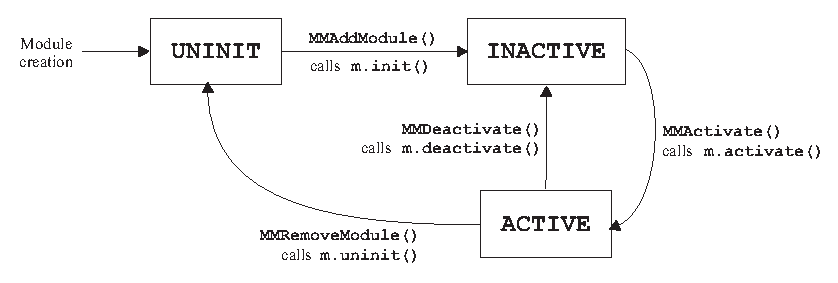
\includegraphics{ModuleLifecycle.eps}}
    \caption{The lifecycle of a module {\tt m}. The boxes represent possible module
      states and the arrows are module manager function calls that affect
      the state of a module.}
    \label{fig:module_lifecycle}
  \end{center}
\end{figure}
%%%%%%%%%%%%%%%%%%%%%%%%%%%%%%%%%%%%%%%%%%%%%%%%


\begin{prototype}
virtual void init( void ) = 0; \\
virtual void uninit( void ) = 0; \\
virtual void activate( void ) = 0; \\
virtual void deactivate( void ) = 0; \\
virtual void update( void ) = 0;
\end{prototype}

These methods define the functionality of a module and are invoked by the
module manager as necessary. The \Module\ base class defines them as pure
virtual functions. It is the responsibility of the programmer to define
these functions in classes derived from the \Module\ base class.

The \initFN\ method is called when a module is ``added'' to the Module
Manager (see \S\ref{sec:mm_add_remove}). Usually, it is only called once. It
should initialize all internal components (i.e.\ allocate memory) and
prepare the module for activation.

The \activateFN\ method is called when the module manager receives a request
to activate a module object. The module manager will start scheduling the
calls to the module's \updateFN\ function once the module has been activated. This
method should initialize all the necessary components of the module,
particularly those that depend on the {\it time} the module was activated,
thereby preparing the \updateFN\ method to be called.

The \updateFN\ method defines the task that the module represents. It is
periodically called by the module manager based on the scheduling parameters
specified at the time the module is added to the system.

The \deactivateFN\ method is called when the module manager receives a
request to deactivate a module object. It should perform any tasks that
depend on the time that the module is deactivated. Following the
deactivation, the module manager will not update the module.

The \uninitFN\ method is called when a module is ``removed'' from the system
(see \S\ref{sec:mm_add_remove}). Usually, it is only called once. It should
clean up all internal components (i.e.\ deallocate memory). The module will
most likely be deleted after this member function is called.

\begin{prototype}
char *getName( void ); \\
int   getIndex( void ); \\
\end{prototype}

These methods are used to access the name and index of a module.

\begin{prototype}
void setName ( char *name );
\end{prototype}
%laura: why do we have this function? it seems useless, and
%potentially dangerous.

This protected method can be used by classes derived from the \Module\ class
to explicitly set the name outside the constructor. However, the name of a
module should, by design, not change after initialization.

\begin{prototype}
\mmstep\ getPeriod( void ); \\
\mmstep\ getOffset( void ); \\
int     getOrder( void );
\end{prototype}

These methods provide access to the period, offset and order parameters of a
module. By definition, the \updateFN\ method of a module is periodically
called (by the Module Manager, see \S\ref{sec:mm_main_loop}) to accomplish the
periodic task the module represents. The {\tt period} and {\tt offset}
parameters determine the periodicity and the beginning time offset of the
first update, respectively. If multiple modules are to be updated in the
same step, the {\tt order} parameter determines the execution order. See
\S\ref{sec:mm_main_loop} for a discussion of module update scheduling.

\begin{prototype}
Module *getNext( void );\\
Module *getPrev( void );
\end{prototype}

The module manager keeps track of all the modules that have been added to it
in one of two linked lists, one for normal modules, the other one for
polling modules. These methods access the next and previous
modules in the list (see \S\ref{sec:mm_add_remove}).
%laura: maybe it would be nice if you explained somewhere why there
%are two linked lists.

\begin{prototype}
Module *getOwner( void );
\end{prototype}

The activation of modules which are configured to be single-user modules
requires the presence of an pointer to an {\it owner} module. The module
manager keeps track of this ownership relation and enforces the single-user
requirement (see \S\ref{sec:mm_activation}). This method returns a pointer
to the current owner of this module or {\tt NULL} if there is no owner at
the time of the call.
%laura: i would mention here that a single-user module does not HAVE
%to have an owner, ie. the pointer to the owner may be NULL.

\begin{prototype}
bool isPolling( void );\\
bool isSingleUser( void );
\end{prototype}

These methods are predicates used to determine if a module is a single-user
and/or a polling module as explained in the constructor function.

\section{The Module Manager}
\label{sec:mm_info}

The \ModuleManager\ class implements a facility to manage all module
activity in the system. The interface to its functionality, however, is not
through its member functions, but through a collection of wrapper
functions. Including the {\tt ModuleManager.hh} file initializes a single
global \ModuleManager\ object. Although the creation of additional
\ModuleManager\ objects is possible, it is not an intended use of the class
and is therefore strongly discouraged. Instead, the global instance
should be used through the wrapper functions described in this section.

The module manager provides many functions for handling modules, accessing
hardware and so on, which are described below. These function are all
prefixed with the letter {\tt MM} and are available by including the {\tt
ModuleManager.hh} file.

\begin{prototype}
\CLOCK\ MMGetStepPeriod( void );
\end{prototype}

This method returns the period of the module manager main loop. The value
returned by this function also corresponds to the real time duration of the
\mmstep\ unit.

\begin{prototype}
\mmstep\ MMGetStepCount( void );
\end{prototype}

This method returns the number of steps that the module manager main loop
has gone through since the beginning of execution. The real time elapsed is
the product of this with the module manager step period.

\section{Choosing and Using The Hardware}
\label{sec:choosing_hardware}

In \rhexlib\, the interface to the low level hardware is accomplished
through the virtual \Hardware\ class (see \S\ref{sec:hardware_class}). To
access critical hardware components such as the real-time clock, the module
manager needs to know about which particular hardware object is to be
used. The function {\tt MMChooseHardware()} is used to inform the module
manager of the hardware object to be used. Once the hardware object is
chosen, the function {\tt MMGetHardware} can be used from within any module
to access the currently chosen hardware object for low level operations.

\section{The Module Manager Main Loop and Module Updates}
\label{sec:mm_main_loop}

\begin{prototype}
void MMMainLoop( void );
\end{prototype}

This function transfers control of a \rhexlib\ program to the module
manager. It never returns and so it should not be called until all modules
to be used have been added to the module manager and the appropriate ones
have been activated. Listing \ref{list:mm_main_loop} shows the basic
functionality of the module manager main loop. The two functions {\tt
updateModules()} and {\tt updatePollingModules()}, called by the main loop
only, determine which modules need their update functions to be called for
normal and polling modules, respectively. Polling modules are updated once
every time the module manager executes the loop. Normal modules, on the
other hand, are statically scheduled for updates based on their parameters.

\begin{codefloat}
\begin{codesegment}
  while ( true ) {
    now = readClock();

    if ( now - clock_mark >= step_period ) {
      while ( now - clock_mark >= step_period )
        clock_mark += step_period;

      updateModules ();
    }
    updatePollingModules ();
  }
\end{codesegment}
\caption{Module manager main loop}
\label{list:mm_main_loop}
\end{codefloat}

The module manager schedules modules at periodic intervals, determined by
the module manager time step (see \S\ref{sec:mm_info}). Listing
\ref{list:mm_update_modules} summarizes the {\tt updateModules()} function,
which updates modules in the appropriate order according to a static
schedule.

\begin{codefloat}
\begin{codesegment}
  m = firstModule;
  while ( m != lastModule ) {

    if ( ( ( current_step - m.getOffset() ) mod m.getPeriod() ) == 0 ) {
      if ( m.getState() == MODULE_ACTIVE)
        current->update();
      m = m.nextModuleInOrder;
    }
  }
\end{codesegment}
\caption{Scheduling of modules in {\tt updateModules()}}
\label{list:mm_update_modules}
\end{codefloat}

\noindent The {\it offset} and {\it period} parameters of a module completely determine its update
schedule. The first update of a module is scheduled {\it offset} steps after
the main loop is invoked. Subsequent updates occur periodically until the
module is deactivated or the module manager shuts down. Note that the
addition and activation times of a module do not affect its update
schedule. Finally, if multiple modules are scheduled for a given step, they
are updated in the increasing order of their {\it order} parameters.

\begin{prototype}
void MMShutdown( void );
\end{prototype}

This function performs a clean shutdown of the module manager. It first
deactivates all the currently active modules and then removes all modules
previously added with the {\tt MMAddModule} function (see
\S\ref{sec:mm_add_remove}). The module objects are not deallocated after
removal.

{\bf Note:} Modules should not directly call this function. Due to the fact that
all modules are removed as a result of this function call, no module update
functions will be called and the module manager loop will run indefinitely.

\begin{prototype}
void MMPowerOff( void );
\end{prototype}

Calls {\tt MMShutdown()} and exits the program. Modules can call this
function to terminate execution (e.g. user interrupt, emergency shutdown
etc.)

% eric: should we say where these functions are called from? otherwise,
% users might think they should call them themselves. 

% uluc: They can call MMPowerOff, but not MMShutdown.
% Actually, I was pondering whether we should just remove MMShutdown() or
% not. I am not entirely happy with the way modules can terminate execution
% for the time being. Maybe we should have a flag or something which will
% exit the module manager loop, at the end of which MMShutdown will be
% called? That look more graceful than just calling MMPowerOff().

%laura: maybe you shouldnt' include MMShutDown in the manual, or else
%include it AFTER MMPowerOff, and make it clear that users should use
%PowerOff.

\section{Adding, Removing and Finding Modules}
\label{sec:mm_add_remove}

\begin{prototype}
void MMAddModule( m, period, offset, order ); \\
Module *m; \\
\mmstep\ period, offset; \\
int order;
\end{prototype}

This function adds the module pointed to by {\it *m} to the current list of
modules with the given {\it period}, {\it offset} and {\it order}
parameters. It calls the \initFN\ method of the module and puts it in the
\ModuleInactive\ state.

\begin{prototype}
void MMRemoveModule( Module *m );
\end{prototype}

This function removes the module pointed to by {\it *m} from the current
list of modules. If the module is active, it is deactivated first, through
{\tt MMRemoveModule()}. Then, the module is removed from the module
manager's list and its \uninitFN function is called.

{\bf Note:} Attempting to remove a module which is in use by another module
generates a fatal error, following which the module manager shuts down and
the program exits after displaying an error message (see
\S\ref{sec:errors}). Details of module ownership are explained in
\S\ref{sec:mm_activation}.

% eric: explain what a fatal error is. 
% uluc: fixed.
%laura: question- just above, did you mean to say it is deactivated 
%first through a call to MMDeactivateModule ?

\begin{prototype}
Module *MMFindModule( char *name, int index );
\end{prototype}

This function returns a pointer to the module with the given name and
index. This is the proper way for a module to locate another module whose
services it requires. It is usually used by a module when it is being added
to the system, i.e.\ from within the module's \initFN\ method.

{\bf Note:} If the specified module has not been previously added, this function
returns {\tt NULL}. Callers should check for this return value and generate
an error if necessary.

% eric: no it doesn't, it returns NULL -- which has to be caught by the user.
% uluc: fixed.

\section{Module Activation, Deactivation and Ownership}
\label{sec:mm_activation}

\begin{prototype}
void MMActivateModule( Module *m );
\end{prototype}

This function puts the module pointed to by {\tt *m} into the \ModuleActive\
state and calls its \activateFN\ function if it was not already in the
\ModuleActive\ state. Following this function call, the \updateFN\ method of
the module's \updateFN\ method will be called by the module manager
according to the module's fixed schedule (see \S\ref{sec:mm_main_loop}).

{\bf Note:} Unless absolutely necessary, {\tt MMGrabModule()} should be used
instead of this function because it keeps track of multiple users for
modules and makes sure modules are not deactivated when they are in use.

% eric: what does static mean?
% uluc: static = fixed, does not change once initialized.

\begin{prototype}
void MMDeactivateModule( Module *m );
\end{prototype}

This function puts the module pointed to by {\tt *m} in the \ModuleInactive\
state and calls its \deactivateFN\ method if it was not already in the
\ModuleInactive\ state. Following this function call, the \updateFN\ method
of the module will not be called until the module is activated again.

{\bf Note:} Unless absolutely necessary, {\tt MMReleaseModule()} should be
used instead of this function because it keeps track of multiple users for
modules and makes sure modules are not deactivated when they are in use.

\begin{prototype}
void MMGrabModule( Module *m, Module *asker );
\end{prototype}

This function is a request to make the module {\tt *asker} become the owner
of the module {\tt *m}. This request is granted if the module does not
already have an owner or the module is not of type {\tt singleUser}. In the
latter case, all grab requests are granted. This function also calls {\tt
MMActivateModule()} in order to activate the module. The module manager
keeps track of a grab count for each module.

This facility is provided to grant exclusive access to modules which use
single-user resources (such as analog outputs). Consequently, upon
activation, all modules should call this function to request ownership for
all the resources they will be using in their updates. It is also good
practice to request ownership for multiple user resources, as it does not
result in any overhead and will ensure proper operation in the future.

% eric: somewhere we should list all the things commonly done in the Module 
% methods, i.e. allocate space, find and grab modules, release modules, etc.
% uluc: How about adding a section: Guidelines for Module design.

{\bf Note:} If the module's {\tt singleUser} flag is true and it is already
owned by another module, this function generates a fatal error, resulting in
the termination of the program. Consequently, the use of {\tt
MMGrabModule()} requires careful design in order to avoid untimely
termination of execution.

% eric: not sure what you mean here.
% uluc: Tried to clarify in the previous Note.

\begin{prototype}
void MMReleaseModule( Module *m, Module *asker );
\end{prototype}

This function releases the ownership of a module. The module is also
deactivated if its grab count reaches zero, meaning that it is not being
used by any other module. Consequently, the grab-release method of
allocating module resources also provides a convenient interface to module
activation and deactivation.

{\bf Note:} If {\tt *m} is owned by some module different than {\tt *asker},
a warning is generated and the module is not released.

\section{Timing Functions}
\index{Timing!functions}

\begin{prototype}
double MMReadTime( void );
\end{prototype}

This function returns the time elapsed in seconds since the invocation of the
program. It uses the {\tt readClock()} method of the low level hardware and
provides a low resolution timing facility.

\begin{prototype}
double MMReadUTime( void );
\end{prototype}

This function returns the time elapsed in seconds since the invocation of
the program at a resolution higher than or equal to that of the {\tt
MMReadClock()} function. It uses the {\tt readUClock()} method of the low
level hardware, and is usually computationally more expensive than its low
resolution counterpart.

\begin{prototype}
\CLOCK\ MMReadClock( void );
\CLOCK\ MMReadUClock( void );
\end{prototype}

These functions are internally used by RHexLib in time computations and
should not be used unless absolutely necessary.

\section{Configuration Facilities}

The \rhexlib module manager keeps a system-wide symbol table for
configuration purposes. Each symbol in the table has a name, which is a
character string, a type (which is either \float\, \floats\, \strings\, or
character string) and a value. As an instantiation of the \SymbolTable\
class, this facility can be used to access system configuration data from
ascii files, avoiding the use of hard coded constants. See
\S\ref{sec:symbol_table} for details on file format and different symbol
types.

\begin{prototype}
void MMReadConfigFile( const char *filename );
\end{prototype}
\index{Configuration files!reading}

This function reads in the specified configuration file into the system
level symbol table.

\begin{prototype}
float MMGetFloatSymbol( const char *name, const float def );
\end{prototype}

This function searches the module manager symbol table for a \float\ typed
symbol with the name {\tt *name}. It returns the value of the symbol. If a
symbol with the given name does not exist or if it has a different type, the
supplied default value is returned.

\begin{prototype}
\floats\ MMGetArraySymbol( const char *name );
\end{prototype}

This function searches the module manager symbol table for a \floats\ typed
symbol with the name {\tt *name}. It returns the value of the symbol in a
\floats\ array. If the symbol with the given name does not exist or has a
different type, an empty array of floats is returned.

\begin{prototype}
strings MMGetStringSymbol( char *name, char *str, char *def );
\end{prototype}

This function searches the module manager symbol table for a string typed
symbol with the name {\tt *name}. It returns the value of the symbol. If a
symbol with the given name does not exist or if it has a different type, the
supplied default value is returned.

%laura: i added this-
\begin{prototype}
void MMGetStrArraySymbol( char *name );
\end{prototype}

This function searches the module manager symbol table for a \strings\ 
typed symbol with the name {\tt *name}. It returns the value of the
symbol in a \strings\ array. If the symbol with the given name does
not exist, of if it has a different type, an empty array of char *s
is returned.

\section{Errors, Warnings and Messages} 
% eric: this section needs to be pointed to from above
% uluc: done.

\label{sec:errors}

The module manager provides several facilities to handle errors and display
warnings and messages. Direct output to {\tt stdout} or {\tt stderr} should
be avoided because they often perturb the real-time performance of the
system. The functions described in this section provide a uniform and
configurable way to handle text output.

Even though the current implementation of these functions simply prints the
messages on the console, future versions will support network
communications, logging to files etc.

\begin{prototype}
void MMFatalError( char *fname, char *msg );
\end{prototype}

This function issues a fatal error and displays a message consisting of the
name of the function supplied in {\tt fname} and the error message in {\tt
msg}. Following the message, it calls {\tt MMPoweroff()} and exits the
program after a clean shutdown of the module manager.

{\bf Note:} A newline is appended at the end of the message text.

\begin{prototype}
void MMWarning( char *fname, char *msg );
\end{prototype}

This function displays a warning message consisting of the name of the
function supplied in {\tt fname} and the warning message in {\tt msg} and
returns.

{\bf Note:} A newline is appended at the end of the message text.

\begin{prototype}
void MMMessage( char *msg );
\end{prototype}

This functon displays the supplied message text and returns. No newline is
appended at the end of the message.

\begin{prototype}
void MMPrintModules( void );
\end{prototype}

This function is mainly for debugging purposes. It displays all the modules
currently maintained by the module manager, together with their state and
parameter information.



%
% This file is part of RHexLib, 
%
% Copyright (c) 2001 The University of Michigan, its Regents,
% Fellows, Employees and Agents. All rights reserved, and distributed as
% free software under the following license.
% 
%  Redistribution and use in source and binary forms, with or without
% modification, are permitted provided that the following conditions are
% met:
% 
% 1) Redistributions of source code must retain the above copyright
% notice, this list of conditions, the following disclaimer and the
% file called "CREDITS" which accompanies this distribution.
% 
% 2) Redistributions in binary form must reproduce the above copyright
% notice, this list of conditions, the following disclaimer and the file
% called "CREDITS" which accompanies this distribution in the
% documentation and/or other materials provided with the distribution.
% 
% 3) Neither the name of the University of Michigan, Ann Arbor or the
% names of its contributors may be used to endorse or promote products
% derived from this software without specific prior written permission.
% 
% THIS SOFTWARE IS PROVIDED BY THE COPYRIGHT HOLDERS AND CONTRIBUTORS
% "AS IS" AND ANY EXPRESS OR IMPLIED WARRANTIES, INCLUDING, BUT NOT
% LIMITED TO, THE IMPLIED WARRANTIES OF MERCHANTABILITY AND FITNESS FOR
% A PARTICULAR PURPOSE ARE DISCLAIMED. IN NO EVENT SHALL THE REGENTS OR
% CONTRIBUTORS BE LIABLE FOR ANY DIRECT, INDIRECT, INCIDENTAL, SPECIAL,
% EXEMPLARY, OR CONSEQUENTIAL DAMAGES (INCLUDING, BUT NOT LIMITED TO,
% PROCUREMENT OF SUBSTITUTE GOODS OR SERVICES; LOSS OF USE, DATA, OR
% PROFITS; OR BUSINESS INTERRUPTION) HOWEVER CAUSED AND ON ANY THEORY OF
% LIABILITY, WHETHER IN CONTRACT, STRICT LIABILITY, OR TORT (INCLUDING
% NEGLIGENCE OR OTHERWISE) ARISING IN ANY WAY OUT OF THE USE OF THIS
% SOFTWARE, EVEN IF ADVISED OF THE POSSIBILITY OF SUCH DAMAGE.

%%%%%%%%%%%%%%%%%%%%%%%%%%%%%%%%%%%%%%%%%%%%%%%%%%%%%%%%%%%%%%%%%%%%%%
% $Id: standardmodules.tex,v 1.9 2001/07/26 05:18:40 ulucs Exp $
%
% Created       : Uluc Saranli, 01/06/2001
% Last Modified : Uluc Saranli, 06/27/2001
%
%%%%%%%%%%%%%%%%%%%%%%%%%%%%%%%%%%%%%%%%%%%%%%%%%%%%%%%%%%%%%%%%%%%%%%

\chapter{Summary of Standard RHexLib Modules}
\label{sec:rhexlib_module_summary}

This section outlines the interfaces and properties of all standard modules
provided with \rhexlib. At the end, Figure \ref{fig:module_summary} presents 
a general view of how these components fit together.

\section{Standard Module Utilities}

In addition to providing a standard set of modules, RHexLib also provides
some utilities to facilitate their use.

\begin{codesegment}
#include "StdModules.hh"
\end{codesegment}

\begin{prototype}
void RHexAddStdModules( void );
\end{prototype}

This function adds all the standard RHexLib modules to the module manager's
list with appropriate periods, offsets and orders. The names, and
scheduling parameters of all the standard modules are defined in {\tt
  StdModules.hh}

\begin{prototype}
void RHexRemoveStdModules( void );
\end{prototype}

This function removes all the standard RHexLib modules to the module manager's
list. Note that this function can only be called after {\tt
  RHexAddStdModules()} is called first.


The following macros define the base orders for different types of
modules. For proper functioning of the system, these macros should be used
when adding modules to be used with the standard set of RHexLib modules.

\begin{datatype}
SENSING\_MODULES \\
USER\_DEFINED\_SENSORS \\
USER\_CONTROLLERS \\
BEHAVIORAL\_CONTROLLERS \\
LOW\_LEVEL\_CONTROLLERS \\
ACTUATOR\_MODULES \\
LOGGING\_MODULES \\
OTHER\_MODULES \\
\end{datatype}

\section{Basic Modules}

\subsection{The \EncoderReader\ Module}

\begin{moduleheader}
\classname{\EncoderReader} \mline
\modulebase{\Module} \mline
\modulename{encreader} \mline
\moduleflags{multi-user, non-polling}
\usedmodules{None}
\end{moduleheader}

The \EncoderReader\ module periodically reads the current count of the
encoder corresponding to its {\tt index} from the system level \Hardware\
object and keeps track of an absolute angular position and velocity for the
corresponding axis. \\

\constructors

\begin{itemize}
\item{\tt EncoderReader ( int index ); }
\end{itemize}

\localinterface

\begin{itemize}
\item{\tt void reset( float pos );}\par
This method sets the current position to {\tt pos}, in radians.
\item{\tt float getPosition( void );} \par 
This method returns the current position in radians, in the range $[-\pi,
\pi]$.
\item{\tt float getSpeed( void );} \par
This method returns the current speed in $rad/s$.
\item{\tt \CLOCK\ getTimestamp( void );} \par
This method returns the timestamp of the latest encoder read.
\end{itemize}

\subsection{The \SpeedFilter\ Module}

\begin{moduleheader}
\classname{\SpeedFilter} \mline
\modulebase{\Module} \mline
\modulename{spdfilter} \mline
\moduleflags{multi-user, non-polling}
\usedmodules{\EncoderReader}
\end{moduleheader}

The \SpeedFilter\ module periodically reads the speed from the
\EncoderReader\ module with the same {\tt index}, and filters the value with
a simple FIR filter. \\

\constructors

\begin{itemize}
\item{\tt SpeedFilter ( int index ); }
\end{itemize}

\localinterface

\begin{itemize}
\item{\tt float getSpeed( void );}\par
This method returns the current filtered speed in $rad/s$.
\end{itemize}

\configsymbols\ None.

\subsection{The \AnalogOutput\ Module}

\begin{moduleheader}
\classname{\AnalogOutput} \mline
\modulebase{\Module} \mline
\modulename{analogout} \mline
\moduleflags{single-user, non-polling}
\usedmodules{None.}
\end{moduleheader}

The \AnalogOutput\ module periodically outputs its current value on the
analog output channel corresponding to its { \tt index} on the system level
\Hardware\ object. \\

\constructors

\begin{itemize}
\item{\tt AnalogOutput ( int index ); }
\end{itemize}

\localinterface

\begin{itemize}
\item{\tt void setValue( float v );}\par
This method sets the current output to {\tt v}, in Volts.
\item{\tt float getValue( void );}\par
This method returns the current output value in Volts.
\end{itemize}

\configsymbols\ None.


\section{Motor Control Modules}

\subsection{The \MotorControl\ Abstract Base Class}

\begin{moduleheader}
\classname{\MotorControl} \mline
\modulebase{\Module} \mline
\moduleflags{single-user, non-polling}
\end{moduleheader}

The \MotorControl\ class is a abstract base class for all modules that
achieve feedback motor control. It enforces a uniform interface to all such
modules. Inherited classes must still provide the {\tt init()}, {\tt
uninit()}, {\tt activate()}, {\tt deactivate()}, {\tt update()} methods.  \\

\constructors

\begin{itemize}
\item{\tt MotorControl( char *name, int index ); }
\end{itemize}

\localinterface

\begin{itemize}
\item{\tt void getGains( MotorGains\_t *g );}\par
This method returns the current motor gains in the struct *g.
\item{\tt void setGains( MotorGains\_t *g );}\par
This method sets the current motor gains to the contents of *g.
\item{\tt void getTarget( MotorTarget\_t *t );}\par
This method returns the current motor target in the struct *t.
\item{\tt void setTarget( MotorTarget\_t *t );}\par
This method sets the current motor target to the contents of *t.
\end{itemize}


\subsection{The \PositionControl\ Module}

\begin{moduleheader}
\classname{\PositionControl} \mline
\modulebase{\Module} \mline
\modulename{poscontrol} \mline
\moduleflags{single-user, non-polling}
\usedmodules{\EncoderReader, \AnalogOutput}
\end{moduleheader}

The \PositionControl\ module performs standard proportional derivative
control over the DC motor corresponding to the module's index number. In
addition to performing position and velocity feedback, it also supports
feedthrough torque commands as well as the ability to configure the type
feedforward compensation.\\

The computed torque command takes the following form.

\begin{equation}
\tau = K_p * e_p + K_d * e_d + \tau_0
\label{eq:torque_feedback}
\end{equation}

where $K_p$ and $K_d$ are the P and D gains, $e_p$ and $e_d$ are the
position and velocity errors and $\tau_0$ is the feedthrough torque setting.

The computation of the position error, due to the rotational nature of the
motor shaft coordinates, requires the definition of an {\em error offset},
$\phi_0$, which is used to determine the range to constrain the position
error term in the above equation.

As a consequence, the cotnroller determines $e_p$ by properly choosing the
integer $k$ in the following equation.

\begin{equation}
e_p = ( \phi_{goal} - \phi ) + 2 k \pi 
\hspace{0.1in}\text{ such that } \hspace{0.1in} 
e_p \in [-\pi+\phi_0, \pi+\phi_0]
\label{eq:pos_error_offset}
\end{equation}

This leverage over the range of the position error on $S_1$ enables features
such as favoring positive ($\phi_0 > 0$) or negative rotation ($\phi_0 < 0$)
of the motor for large position errors (avoiding springback of the leg). Note
that $\phi_0$ cannot be too close to either $\pi$ or $-\pi$ because then,
even when the position of the leg is slightly different than the desired
position, the leg might try to rotate from an unreasonable
direction. Usually, choosing $\phi_0 \in [-\pi/2, \pi/2]$ is a good idea.

Once the torque command is computed, the desired voltage command at motor
terminals is computed using the torque constant of the motor as well as a
feedforward compensation term depending on the current compensation
mode. Currently supported modes are {\tt NONE} and {\tt BACKEMF}.\\

\constructors

\begin{itemize}
\item{\tt PositionControl ( int index ); }
\end{itemize}

\localinterface

\begin{itemize}
\item{\tt void setTorqueOffset( float torque );}\par
This method sets the feedthrough torque value $\tau_0$ of Equation
\ref{eq:torque_feedback}.

\item{\tt void setErrorOffset( float offset );}\par
This method sets the position error offset value $\phi_0$ of Equation
\ref{eq:pos_error_offset}.

\item{\tt float getErrorOffset( void );}\par
This method returns the current setting of $\phi_0$.

\item{\tt void setCompensationType( CompensationType type );}\par
This method sets the type of the feedforward voltage compensation in
computing the motor terminal voltage to be commanded to the physical
hardware. Currently, the position control module assumes that the low level
motor drive circuitry operrates in voltage mode. This requires feedforward
compensation to obtain approximate torque control. The currently supported
types, {\tt NONE} and {\tt BACKEMF} can be used to select the type of the
compensation used by the controller.

\item{\tt CompensationType getCompensationType( void );}\par
This method returns the current type of feedforward voltage compensation.

\item{\tt void freeze( void );}\par
This method freezes the motor position by setting the current motor target 
to the current motor position.
\end{itemize}

\configsymbols\ None.

\section{State Machine Tools}

\subsection{The \StateMachine\ Abstract Base Class}

The \StateMachine\ class is the abstract base class for all state machine
implementations. It defines a uniform interface for defining and running
state machines, automatically handling event checking and state
transitions. There are three related classes: {\tt State}, {\tt Event} and
{\tt Arc}. The first two are abstract base classes. A {\tt StateMachine}
class contains a list of its {\tt State} classes, which are all derived from
the state class. Each state contains a list of arcs, which consist of an
{\tt Event} object and another {\tt State}.

The {\tt Event} abstract base class has the following form.

\begin{moduleheader}
\classname{{\tt Event} } \mline
\modulebase{None} \mline
\end{moduleheader}

\constructors

\begin{itemize}
\item {\tt Event( StateMachine * p );}\par
{\tt p} should point to the {\tt StateMachine} class that owns the event
\end{itemize}

\localinterface

\begin{itemize}
\item{\tt virtual bool check( void );} \par
must be defined by children classes
\end{itemize}

\noindent Programmers can use the {\tt EventObject} macro in the following
way to define new events classes derived from {\tt Event}. This is usually
done in class definition of a machine derived from a state machine so that
the scope of the new class is limited to the derived state machine class.

\begin{codesegment}
  EventObject( NewEvent ) * newEvent;
\end{codesegment}

\noindent This defines a new class called NewEvent which is derived from
{\tt Event}. It declares itself a friend of the containing class, and then
defines {\tt newEvent} to be a pointer to a {\tt NewEvent} object. It is a
programming conventon in RHexLib that event classes are capitalized and
event objects have the same name only with the first symbol in lowercase.

Arcs or {\em transitions} are instantiations of the {\tt Arc} class:

\begin{moduleheader}
\classname{{\tt Arc}} \mline
\modulebase{None} \mline
\end{moduleheader}

\constructors

\begin{itemize}
\item {\tt Arc( State * s, Event * e );}
\end{itemize}

\localinterface

\begin{itemize}
\item{\tt State * getTarget( void );} \par
returns the destination state of the arc 
\end{itemize}

Finally, states must be derived from the {\tt State} abstract base class. 

\begin{moduleheader}
\classname{{\tt State}} \mline
\modulebase{None} \mline
\end{moduleheader}

\constructors

\begin{itemize}
\item{\tt State( StateMachine * p );}
\end{itemize}

\localinterface

\begin{itemize}
\item{\tt void addArc ( Arc * a );} \par
This method adds the arc {\tt a} to the state's outgoing arcs.
\item{\tt Arc * getActiveArc ( void );} \par
Returns first arc leaving state whose event is true (or {\tt NULL} if no
such arc)
\item{\tt virtual void entry ( void );} \par
must be defined by child classes
\item{\tt virtual void during ( void );} \par
must be defined by child classes
\item{\tt virtual void exit ( void );} \par
must be defined by child classes
\end{itemize}

\noindent Programmers may use the {\tt StateObject} macro to define new
state classes within the scope of a {\tt StateMachine} derived class as
follows:

\begin{codesegment}
  StateObject( NewState ) * newState;
\end{codesegment}

\noindent The naming convention for derived state classes is the same as for
events. Programmers may add new outgoing arcs to a state using the {\tt
addArc} method or more conveniently using the {\tt Transition} macro as
follows:

\begin{codesegment}
  Transition ( fromState, anEvent, toState );
\end{codesegment}

\noindent which is syntactic sugar for

\begin{codesegment}
  fromState->addArc ( toState, anEvent );
\end{codesegment}

The {\tt StateMachine} class is as follows.

\begin{moduleheader}
\classname{\StateMachine} \mline
\modulebase{\Module} \mline
\moduleflags{single-user, non-polling}
\usedmodules{None}
\end{moduleheader}

The \AnalogOutput\ module periodically outputs its current value on the
analog output channel corresponding to its { \tt index} on the system level
\Hardware\ object. \\

\constructors

\begin{itemize}
\item{\tt StateMachine( char *n );}
\item{\tt StateMachine( char *n, State *initial );}
\item{\tt StateMachine( char *n, uint index );}
\item{\tt StateMachine( char *n, uint index, State *initial );} 
\end{itemize}

\localinterface

\begin{itemize}
\item{\tt void initialize( State *i );} \par
This method sets the initial state to *i.
\end{itemize}

\noindent Note that state machines are modules and thus have the methods
{\tt activate}, {\tt update} and so on, except that they are not virtual and
thus derived classes do not have to define them, although in practice they
usually do. The {\tt update} function of a {\tt StateMachine} class is quite
simple and is shown below. The private variable {\tt current} points to the
currently active state.

\begin{codesegment}
  void StateMachine::update( void ) {

    Arc * a = current->getActiveArc();

    if ( a != NULL ) {

      current->exit();
      current = a->target;
      current->entry();
    }

    current->during();
  }
\end{codesegment}

\noindent Thus, a {\tt StateMachine} acts like its currently active state
{\em and} checks for active arcs leaving the current state, switching states
to the destination state of the arc if it finds any.

\section{Controller Suite}

\subsection{The \CalibMachine\ Module}
\label{sec:calib_machine}

\begin{moduleheader}
\classname{\CalibMachine} \mline
\modulebase{\StateMachine} \mline
\modulename{calibmachine} \mline
\moduleflags{single-user, non-polling}
\usedmodules{\AnalogOutput, \EncoderReader, \SpeedFilter, \StallSensor,
  \PositionControl.}
\end{moduleheader}

The \CalibMachine\ module is a controller that performs motor drive and
encoder homing calibration. Upon activation, it detects motor polarity,
calibrates the encoders to the correct absolute position and finally
determines the analog output voltage for zero command.\\

Figure \ref{fig:calibmachine} illustrates the state transition diagram for
the calibration state machine. The shaded regions indicate states related to
polarity, encoder and drive calibration algorithms.

%%%%%%%%%%%%%%%%%%%%%%%%%%%%%%%%%%%%%%%%%%%%%%%%
\begin{figure}[!ht]
  \centering
  \epsfig{figure=CalibMachine.eps,width=5.8in}
  \caption{\CalibMachine\ state transition diagram.}
  \label{fig:calibmachine}
\end{figure}
%%%%%%%%%%%%%%%%%%%%%%%%%%%%%%%%%%%%%%%%%%%%%%%%

The polarity calibration is designed to determine the connection polarity of
the motor terminals. Incorrect polarity information will result in unstable
behavior in the local PD feedback control. The algorithm to determine the
polarity is very simple. It starts by applying a positive voltage to the
motor terminals, recording rotational velocity, determining connection
polarity. If, however, the leg is stuck on the ground and is unable to
rotate (stallEv), then it retries with a negative voltage, which will yield
the polarity information if the leg is not permanently stuck.

The calibration of the encoders is a good deal more complicated. The manual
calibration is the simplest. The {\tt encManualCalib} state simply assumes
that the current position of the legs corresponds to leg angles specified in
the {\tt manual\_offset} configuration variable and resets the encoders
accordingly.

In contrast, ground calibration rotates the legs in the positive direction
until they hit the ground, and then resets the encoder angles assuming that
the legs are at angles specified by the {\tt ground\_offset} configuration
variable.

Finally, the home switch calibration relies on the presence of home switches
triggered at a certain angle of the leg. The calibration machine assumes
that the {\tt SwitchHW} component of the low level hardware provides the
outputs of these switches at indices 8 through 13, so that their value is
{\tt true} when the leg triggers the switch. The algorithm starts by
rotating the legs in the positive direction until they either hit the ground
or trigger the switch. If they trigger the switch, it waits until the leg
clears the switch, then starts rotating in the opposite direction to
approach the switch from the correct side. This is important because the leg
angle triggering the switch from different rotational directions will be
different. If, on the other hand, the leg hits the ground, the algorithm
immediately starts seeking the switch by rotating the leg in the negative
direction. 

When the switch is detected while the leg is rotating in the negative
direction, the encoder angles are reset with the angles specified by the
configuration variable {\tt switch\_offset}.

\constructors

\begin{itemize}
\item{\tt CalibMachine( int index ); }
\end{itemize}

\localinterface

\begin{itemize}
\item{\tt CalibStatus getStatus( void ); } \par
This method returns the current calibration status.

\item{\tt void reset( void );} \par
This method invalidates the polaritym encoder and drive calibrations,
causing the machine to perform calibration after the next activation. Note
that the invalidation of the polarity depends on the compile time
configuration of CalibMachine which by default disables the polarity
detection unless the low level hardware does not provide polarity information.

\item{\tt void reset( bool polarity, bool encoder, bool drive );} \par
This method selectively invalidates polarity, encoder and/or drive
calibration. Note that the invalidation of the polarity depends on the
compile time configuration of CalibMachine which by default disables the
polarity detection unless the low level hardware does not provide polarity
information.

\item{\tt void setMode( CalibMode m ); } \par
This method chooses the type of calibration to be used in the next
activation.

\item{\tt CalibMode getMode( void ); } \par
This method returns the current calibration mode

\item{\tt void setUpside( bool down ); } \par
This method chooses whether the body should be assumed to be upside down or
not.  If already calibrated, it resets the encoder reader modules to reflect
the change.

\item{\tt bool isUpsideDown( void ); } \par
This method returns the current assumption for the body orientation.

\end{itemize}

\datatypes

\begin{itemize}
\item{\tt typedef enum CalibMachine::CalibStatus \{ \par
CalibMachine::CALIBRATING, \par
CalibMachine::FAILURE, \par
CalibMachine::SUCCESS  \par \}}\par

This datatype is used to indicate the current status of the calibration
state machine.

\item{\tt typedef enum CalibMachine::CalibMode \{ \par
CalibMachine::MANUAL, \par
CalibMachine::GROUND, \par
CalibMachine::SWITCH \par \} }\par

This datatype is used to configure the calibration state machine to use one
of the supported calibration modes. Currently, three modes are supported:
{\em manual calibration}, which assumes that the legs are statically
positioned by the operator to a predetermined angle; {\em ground
  calibration}, which brings the legs forward to touch the ground and
assumes a particular offset for the legs when they are n contact wioth the
ground, and finally, {\em home switch calibration}, which uses Hall effect
sensors on the hips to calibrate the encoder offsets.
\end{itemize}

\configsymbols

\begin{itemize}

\symbolitem{\tt manual\_offset}\par
This numeric array symbol configures the angles of all six legs when the
legs are manually positioned for manual encoder calibration.

\symbolitem{\tt ground\_offset}\par
This numeric array symbol configures the angles of all six legs when the
legs are touching the ground towards the back of the robot when the robot's
right side is up. These angles are used in the ground encoder calibration.

\symbolitem{\tt switch\_offset}\par
This numeric array symbol configures the angles of all six legs when the
legs trigger the home switch (hall effect sensor) while rotating in the
negative direction. These angles are used during home switch encoder
calibration.

\symbolitem{\tt calib\_timeout}\par
Maximum allowed time for calibration attempts (usec)

\symbolitem{\tt calib\_command} \par
Voltage command for the ground seeking behavior and drive calibration (V)

\symbolitem{\tt calib\_min\_speed} \par
Minimum required motor speed for polarity calibration (rad/s)

\symbolitem{\tt calib\_pol\_time} \par
Minimum required time of nonzero rotation for polarity calibration (usec)

\symbolitem{\tt calib\_stall\_time} \par
Stall time threshold for ground encoder calibration (usec)

\symbolitem{\tt calib\_stall\_toler} \par
Maximum allowed motor rotation speed, still interpreted as stall (rad/s)

\symbolitem{\tt calib\_grnd\_retry} \par
Flag to indicate whether the home switch encoder calibration should fallback
to ground encoder calibration upon failure.

\end{itemize}

\subsection{The \WalkMachine\ Module}
\label{sec:walk_machine}

\begin{moduleheader}
\classname{\WalkMachine} \mline
\modulebase{\StateMachine} \mline
\modulename{walkmachine} \mline
\moduleflags{single-user, non-polling}
\usedmodules{\PositionControl, \EncoderReader.}
\end{moduleheader}

The \WalkMachine\ module is a controller which implements the two-stroke
alternating tripod controller, parametrized by the stride period as well as
duty factors, sweep angles and leg offsets for individual legs. It supports
walking forward and backward, turning in place and differential turning,
even when the robot is upside down. All the functionality can be configured
through the module's local interface. As such, the \WalkMachine\ does not
make any adjustments such as responding to the remote control etc. itself,
and needs a ``supervisor'' to modulate its behavior. \\

\constructors

\begin{itemize}
\item{\tt WalkMachine( void ); }
\end{itemize}

\datatypes

The WalkMachine defines a class datatype to encapsulate the standard
parameters of walking behavior. It takes the form of a class with proper
copy constructors to correctly handle copying of its instances. All of its
member variables are defined public and can be accessed by anyone.

\begin{classdef}
class WalkParam_t {

public:
  WalkParam_t( void ) { };
  WalkParam_t( WalkParam_t & );

  WalkParam_t& operator=( const WalkParam_t & );

public:

  float dutyFactor[6];   // Ratio of slow time to period of rotation
  float sweepAngle[6];   // Angle span during the slow leg sweep
  float legOffset[6];    // Angle offset for the whole profile
  MotorGains_t gains[6]; // Walking motor gains

  double cpgPeriod;      // Period of the whole step cycle    
  double tripodTime;     // Time to prepare and bring down the first tripod
  double standAdjTime;   // Leg offset adjustments time interval while standing
  float turnOffset;      // Differential leg offset adjustment for turning 
  float turnSweepAngle;  // Differential sweep angle adjustment for turning
  float turnDutyFactor;  // Differential duty factor adjustment for turning
  float smooth;          // Ratio for the smoothing speed transitions
  bool cubic;            // Flag to choose between linear or cubic spline smoothing
};
\end{classdef}

\localinterface

\begin{itemize}
\item{\tt void setSpeedCommand( float cmd ); } \par
This method sets the speed command of the walking controller. This
command must be either $-1$, $0$, or $1$.
\item{\tt void setTurnCommand( float cmd ); } \par
This method sets the turning command of the walking controller. A
command $-1$ indicates turning left, $1$ indicates turning right and $0$
indicated no turning.
\item{\tt void setUpside( bool down ); } \par
This method can be used to set the walking controllers assumption
about the robots body orientation. {\tt setUpside( false ) } configures
upside down operation.
\item{\tt void setParams( WalkParam\_t *p ); } \par
This method can be used to set all the walking parameters, modulating
the walking behavior. The parameters are updated only at
half cycles. Moreover, the pointer to the parameter settings is stored,
so any subsequent changes to the contents of {\tt *p} will also change
walking behavior.
\item{\tt void getParams( WalkParam\_t *p ); } \par
This method returns the current walking parameters in {\tt *p }. 
\item{\tt bool isDone( void ); } \par
This method returns a flag indicating whether the walking controller
is done with its operation, which means that both speed and turn
commands are zero and both tripods are lowered.
\end{itemize}

\configsymbols\ None.

\subsection{The \RHexWalker\ Module}
\label{sec:rhexwalker}

\begin{moduleheader}
\classname{\RHexWalker} \mline
\modulebase{\Module} \mline
\modulename{rhexwalker} \mline
\moduleflags{single-user, non-polling}
\usedmodules{\WalkMachine, \SlopeEstimator.}
\end{moduleheader}

The \RHexWalker\ module is a controller which implements variable speed
two-stroke alternating tripod gait with inclination compensation and
variable speed alternating triwheel gait. It accomplishes this by modulating
parameter settings of \WalkMachine, in a way that is adjustable through
configuration files.

The alternating tripod gait is the standard walking algorithm for RHex,
which is used when it has non-circular legs mounted. Section
\ref{sec:walk_machine} summarizes the parameters which modulate the walking
behavior. The RHexWalker module supports variable speed walking, but
choosing parameter values from a piecewise linear interpolation of several
experimentally tuned parameter sets. Several configuration variables define
these various sets and how the interpolation is achieved.

The inclination compensation of the walking gait involves adjusting some of
the walking parameters based on an estimate of the slope through the
\SlopeEstimator\ module. When it is disabled, the leg offsets can also be
manually adjusted through the {\tt setLegOffset()} method call.

The triwheel gait can be used when RHex has circular legs mounted. This gait
also relies on using \WalkMachine, but the parameters are chosen in a very
particular manner. First of all, three of the parameters are kept constant
(with the exception of differential turning): duty factor at $0.5$, leg
offset at $0$ and sweep angle at $\pi$. The period of leg rotation
determines the effective speed, and that parameter is modulated through the
{\tt setForwardCommand()} method. Note that the triwheel gait does not have
inclination compensation and the leg offset cannot be changed. Once again,
the behavior of the speed control and the gait can be adjusted through the
configuration file (see symbol descriptions below).\\

\constructors

\begin{itemize}
\item{\tt RHexWalker( void ); }
\end{itemize}

\localinterface

\begin{itemize}
\item{\tt void setGait( WalkingGait newGait ); }\par
This method sets the walking gait to be used by \RHexWalker. Two gaits are
currently supported {\tt TWO\_STROKE\_TRIPOD\_GAIT} and {\tt
  TRIWHEEL\_GAIT}. The new gait setting becomes effective next time the
module is activated, so changing gaits during walking is not possible.

\item{\tt void setForwardCommand( float cmd ); }\par
This method sets the forward command of the walking controller in the range
$[-1, 1]$. It supports variable speed walking, where the magnitude of the
forward speed command determines the \WalkMachine\ parameters to be used
based on configuration file settings and the current gait (see below).

\item{\tt void setTurnCommand( float cmd ); }\par
This method sets the turning command of the walking controller in the range
$[-1, 1]$. For differential turning, it performs on/off control. For turning
in place, tt supports variable speed turning, where the magnitude of the
speed command determines the \WalkMachine\ parameters to be used
based on configuration file settings and the current gait (see below).

\item{\tt void inclineEnable( bool enable ); }\par
This method can be used to enable/disable the inclination compensation for
the alternating tripod gait. Enabling the inclination compensation overrides
the manual leg offset setting.

\item{\tt void setLegOffset( float offset ); }\par
This method manually sets the leg offsets for all the legs. It is effective
only when the inclination compensation is disabled.

\item{\tt void setUpside( bool down ); }\par
This method can be used to set the walking controllers assumption
about the robots body orientation. {\tt setUpside( false ) } configures
upside down operation.

\item{\tt bool isDone( void ); }\par
This method returns a flag indicating whether the walking controller is
ready to exit or not. Supervisors should check this flag before deactivating
RHexWalker.
\end{itemize}

\configsymbols

\begin{itemize}
\symbolitem{\tt walk\_speeds}\par
This numeric array symbol gives a set of ``speed setting'' indices, to which
the parameter settings of the alternating tripod controller will
correspond. This way, the user can configure experimentally tuned speed
settings to irregularly spaced intervals. For example, if you have
parameters for a very slow walk, and then two other parameter sets for fast
walking with slightly different speeds, {\tt walk\_speeds = \{ 1.0 9.0 10.0
  \}} would be a good setting. Most of the symbols below with the prefix
{\tt walk} must have the same number of array elements as this symbol.

If {\tt walk\_speeds} is not defined, only the first elements of the array
symbols below are used for all speed settings and the variable speed feature
is disabled.

\symbolitem{\tt walk\_tripod\_time}\par
This numeric array symbol configures the time spent to prepare the tripod
before the walking starts as well as to bring the upper tripod down when it
stops. Each of the array entries correspond to one of the speed indices and
for a given speed setting, the value of this parameter is linearly
interpolated between the two enclosing values. If {\tt walk\_speeds} is not
defined, only the first number in the array is used for the parameter.

\symbolitem{\tt walk\_cpg\_period}\par
This numeric array symbol configures the rotation period of all the
legs. The semantics of the array elements are the same as the {\tt
  walk\_tripod\_time} symbol.

\symbolitem{\tt walk\_duty\_factor}\par
This numeric array symbol configures the ratio of the slow period of all the
legs to the overall rotational period. The semantics of the array elements
are the same as the {\tt walk\_tripod\_time} symbol.

\symbolitem{\tt walk\_sweep\_angle}\par
This numeric array symbol configures the angle span of the slow leg rotation
phase. The semantics of the array elements are the same as the {\tt
  walk\_tripod\_time} symbol.

\item{\tt walk\_leg\_offset\_forward, walk\_leg\_offset\_backward}\par
\symbolindex{\tt walk\_leg\_offset\_forward}
\symbolindex{\tt walk\_leg\_offset\_backward}
These numeric array symbols configure the angular offset of the whole leg
profile with respect to the vertical. The semantics of the array elements
are the same as the {\tt walk\_tripod\_time} symbol.

\symbolitem{\tt walk\_cubic}
This numeric symbol defines whether cubic smoothing is enabled for the
profile generation of the alternating tripod walking controller.

\symbolitem{\tt walk\_smooth\_factor}\par
If the cubic smoothing is enabled, this numeric array symbol configures what
percentage of the leg rotation period should be used for the smoothing. Once
again, the corresponding \WalkMachine\ parameter is interpolated as in the
{\tt walk\_tripod\_time} symbol.

\item{\tt walk\_turn\_offset, walk\_turn\_sweep\_angle,
    walk\_turn\_duty\_factor}\par
\symbolindex{\tt walk\_turn\_offset}
\symbolindex{\tt walk\_turn\_sweep\_angle}
\symbolindex{\tt walk\_turn\_duty\_factor}
These numeric array symbols configure how much differential adjustment will
be made to contralateral legs during differential turning for the
corresponding parameters.  The interpolation of the parameters
are done the same as they were for {\tt walk\_tripod\_time} symbol.

\symbolitem{\tt triwheel\_tripod\_time}\par
This numerical symbol tripod preparation and lowering time for the triwheel
gait. This gait does not incorporate parameter interpolation, so this symbol
is only a number.

\item{\tt triwheel\_min\_cpg\_period, triwheel\_max\_cpg\_period}\par
\symbolindex{\tt triwheel\_min\_cpg\_period}
\symbolindex{\tt triwheel\_max\_cpg\_period}
These numerical symbols configure the minimum and the maximum leg rotation
period for the variable speed control of the triwheel gait. Based on the
forward command setting, \RHexWalker\ chooses a value in between to obtain
different walking speeds.

\symbolitem{\tt triwheel\_turn\_sweep\_angle}\par
This numerical symbol configures the differential adjustment in the sweep
angles of contralateral legs to obtain differential turning in the triwheel
controller. Once again, there is no interpolation involved, so this symbol
does not require an array input.
\end{itemize}

\subsection{The \StandMachine\ Module}
\label{sec:stand_machine}

\begin{moduleheader}
\classname{\StandMachine} \mline
\modulebase{\StateMachine} \mline
\modulename{standmachine} \mline
\moduleflags{single-user, non-polling}
\usedmodules{\PositionControl, \EncoderReader.}
\end{moduleheader}

The \StandMachine\ module is a controller which stands the robot up from a
stationary position. Once activated, it commands the legs first to go to a
horizontal position, and then go downwards in synchrony to push the body
up. \\

\constructors

\begin{itemize}
\item{\tt StandMachine( void ); }
\end{itemize}

\localinterface

\begin{itemize}
\item{\tt void setParams( StandParam\_t *p ); } \par
This method can be used to set all the standing parameters. See
\S\ref{sec:special_types} for an explanation of the data type {\tt
  StandParam\_t}.
\item{\tt void getParams( StandParam\_t *p ); } \par
This method returns the current standing parameters in {\tt *p }.
\item{\tt bool isDone( void ); } \par
This method returns a flag indicating whether the standing controller
is done with its operation, which means that all leg targets have
reached the vertical position.
\end{itemize}

\configsymbols

\begin{itemize}
\symbolitem{\tt stand\_one\_time}\par
This numeric symbol configures the time in seconds for the legs to get into
horizontal position.
\symbolitem{\tt stand\_two\_time}\par
This numeric symbol configures the time in seconds for the legs to get lift
the body up from their horizontal position.
\symbolitem{\tt stand\_adj\_time}\par
This numeric symbol configures the period between succesive leg offset
adjustments at the end of standing. Primarily used for runtime adjustment
leg offset for things like inclination compensation. The {\tt
  setLegOffset()} should be used for such compensation actions.
\symbolitem{\tt stand\_kp}\par
This numeric array variable configures the proportional gains for the legs
during standing.
\symbolitem{\tt stand\_kd}\par
This numeric array variable configures the derivative gains for the legs
during standing.
\end{itemize}

\subsection{The \SitMachine\ Module}
\label{sec:sit_machine}

\begin{moduleheader}
\classname{\SitMachine} \mline
\modulebase{\StateMachine} \mline
\modulename{sitmachine} \mline
\moduleflags{single-user, non-polling}
\usedmodules{\PositionControl, \EncoderReader.}
\end{moduleheader}

The \SitMachine\ module is a controller which makes the robot sit down from
a standing position. Once activated, the algorithm commands the legs to go
to a horizontal position, lowering the robot to the ground. \\

\constructors

\begin{itemize}
\item{\tt SitMachine( void ); }
\end{itemize}

\localinterface

\begin{itemize}
\item{\tt bool isDone( void ); } \par
This method returns a flag indicating whether the sitting controller
is done with its operation, which means that all leg targets have
reached the horizontal position.
\end{itemize}

\configsymbols

\begin{itemize}
\symbolitem{\tt sit\_time}\par
Time to bring the legs to their horizontal position (sec).
\end{itemize}

\section{Utility Modules}

\subsection{The \DataLogger\ Abstract Base Class}

\begin{moduleheader}
\classname{\DataLogger} \mline
\modulebase{\Module} \mline
\moduleflags{single-user, non-polling}
\usedmodules{None}
\end{moduleheader}

The DataLogger class is a general purpose utility to store data vectors in
memory while the robot is operational and save them later to files in a
variety of data formats. It is defined as an abstract base class. As a
consequence, it cannot be directly instantiated. Instead, a new class must
be derived from DataLogger, choosing the size of the data vector and the
contents of the log.

The period of the module when added with the {\tt MMAddModule()} function
call determines the frequency at which the data vector is logged. Moreover,
the {\tt logging\_period} symbol provides means of configuring this frequency
independent of the module's own period. Please see the symbol explanation
below for details.

\constructors

\begin{itemize}
\item{\tt DataLogger( void );} \par

This constructor creates a DataLogger with the default name "datalogger",
index 0 and a data vector length of 1. These values, except the record
length, cannot be changed once the class is instantiated, which is also true
for all the other constructors of DataLogger.

\item{\tt DataLogger( int reclen );} \par

This constructor creates a DataLogger with the default name "datalogger",
module index 0 and a data vector length of {\tt reclen}. 

\item{\tt DataLogger( int reclen, int index );} \par

This constructor creates a DataLogger with the default name "datalogger",
the specified {\tt index} and a data vector length of {\tt reclen}.

\item{\tt DataLogger( int reclen, char *name );} \par

This constructor creates a DataLogger with the specified {\tt name},
index 0 and a data vector length of {\tt reclen}.

\item{\tt DataLogger( int reclen, char *name, int index );} \par

This constructor creates a DataLogger with the specified {\tt name},
{\tt index} and a data vector length of {\tt reclen}.

\end{itemize}

\localinterface

\begin{itemize}
\item{\tt virtual void  fillRecord ( float *f ) = 0;} \par
This method is a pure virtual function and needs to be defined by the
inherited classes. It is where the contents of the data vector to be logged
are filled in. The inherited definition must fill in the contents of the
vector {\tt *f} with whichever variables need to be logged.

\item{\tt void reset( void );} \par
This method resets the contents of the DataLogger by deleting all previously
logged data.

\item{\tt void reset( int new\_reclen );} \par
This method also resets the contents of the DataLogger by deleting all
previously logged data. However, in doing so, it also sets the data vector
length of the logger to {\tt new\_reclen}.

\item{\tt void setLoggingPeriod( int p );} \par
This method sets the logging period for the logger, overriding the value
chosen through the {\tt logging\_period} configuration symbol. The unit of
{\tt p} is module manager steps (also milliseconds in the current
implementation).

\item{\tt void exportToFile ( char *basefilename, DL\_OUTPUT\_TYPE type, char** names );} \par
This method dumps the current contents of the logger into a file specified
by {\tt *basefilename}. The suffix {\tt .data} is appended to the end of
this base filename.

The next two arguments are optional and can be left unspecified. The {\tt
type} argument specifies the type of the output file. Currently the only
supported type is {\tt DL\_ASCII}, which outputs columns of ascii
numbers. The default value for this argument (if left unspecified), is {\tt
DL\_ASCII}.

The {\tt names} argument can be used to specify names for the variables that
are being logged. This method then creates a Matlab executable file, {\tt
  basefilename.m}, which, when executed from within Matlab, loads the
corresponding data file and assigns Matlab variables with the specified
names to appropriate columns of the data. If {\tt NULL} is passed, the data
logger does not generate this file. The default value, in case this argument
is left unspecified) is {\tt NULL}.

\item{\tt int exportViaNet( char *basefilename, DL\_OUTPUT\_TYPE type, char
**names );} \par 
This method has very similar functionality to the method {\tt
exportToFile()}. However, after writing the data files to disk, this
function transfers them over the network to the host specified by the {\tt
rhexftphost} config symbol into the directory specified by {\tt
rhexftppath}. Moreover, the configuration symbols {\tt rhexftpuser} and {\tt
rhexftppasswd} must be assigned with the username and password on the target
host.
\end{itemize}

\configsymbols

\begin{itemize}

\symbolitem{\tt logging\_period}\par 

This numeric config symbol specifies the period of logging in milliseconds
(more accurately, module manager steps). It takes into account the module
period of the data logger, but the logging period is not an integer multiple
of the module period, the actual time difference between data samples might
be somewhat uneven. The default is 1.

\symbolitem{\tt rhexftphost}\par
This string config symbol specifies the hostname for FTP transfer of the
data files exported through  {\tt int exportViaNet()}.
\symbolitem{\tt rhexftppath}\par
This string config symbol specifies the target directory for FTP transfer of
the data files exported through  {\tt int exportViaNet()}.
\symbolitem{\tt rhexftpuser}\par
This string config symbol specifies the username on the target host for FTP
transfer of the data files exported through  {\tt int exportViaNet()}.
\symbolitem{\tt rhexftppasswd}\par
This string config symbol specifies the password on the target host for FTP
transfer of the data files exported through  {\tt int exportViaNet()}.
\end{itemize}

\examplecode

Here is an example of how to define a data logger class, inherited from
DataLogger.

\begin{codesegment}
class ExampleLogger : public DataLogger {
  public:
    ExampleLogger( void ) : DataLogger( 2, "examplelogger", 0);

    void fillRecord( float *f ) {
      f[0] = MMReadTime();
      f[1] = sin( 2.0 * M_PI * MMReadTime() );
    }
};
\end{codesegment}

This code segment defines an ExampleLogger module, with name {\tt
"examplelogger"} and index 0, logging the array \{$t$, $\sin t$\}. Note that
this module must be explicitly created and added to the module manager
somewhere (usually in main()) to be of any use.

*WARNING* : If you redefine any of the module functions, you must explicitly
call the corresponding method of the DataLogger base class at the end of the
module function. For example, if ExampleLogger were to redefine the init()
module function, it would have to look like this:

\begin{codesegment}
ExampleLogger::init( void ) {

  ( some code goes here.... )

  DataLogger::init();
};
\end{codesegment}

Otherwise, the data logging functionality will not work properly.

\subsection{The \RHexLogger\ Generic Logging Module}

\begin{moduleheader}
\classname{\RHexLogger} \mline
\modulebase{\Module} \mline
\moduleflags{single-user, non-polling}
\usedmodules{\DataLogger}
\end{moduleheader}

This module provides a variety of logging options, including a set of 140
standard variables, 16 global variables as well as functionality to add new
named variables to be logged at runtime. The set of variables to be logged
each time the program is run is determined by the configuration file (see
the symbol explanations below), so subsequent runs may log different
variables without recompilation. All relevant configuration files should be
read {\em before} the RHexLogger module is created (i.e. before {\tt
RHexAddStdModules()} or similar functions are called).\\

When exporting data to a file (or over the network), RHexLogger also creates
supplies the DataLogger (see above) with the names of the variables,
generating an associated Matlab file to load the variables into the Matlab
workspace with the same names. A very useful feature of RHexLogger is the
ability to include the current date, time and a unique log index as part of
the filename specification in the configuration file using the identifiers
{\em \%d \%t} and {\em \%i}.

An array of 16 floating point global variables {\tt rhexLoggerGlobalVars}
are defined by RHexLogger with the names {\tt user\_defined0} through {\tt
user\_defined15}. When these variables are enabled for logging in the config
file, RHexLogger records the values of these global variables. This facility
can be used for quick debugging, where you can simply assign the value you
would like to be logged to one of these global variables. Unfortunately, it
is not possible to change the names of these variables.

Another custom functionality is the ability to add new variables to be
logged at runtime. This is is mostly for debugging purposes as it requires
recompilation for adding and removing new variables. However it does present
the ability to define variables with custom names, which is useful for
archiving the data files with more meaningful names for custom variables
than {\tt user\_defined5}. This is accomplished through the methods {\tt
  addNewVar()} and {\tt addNewFunc()}. These function must be called {\em
  after} the RHexLogger has been created and added to the module manager
(i.e. after RHexAddStdModules() has been called). The newly added variables
are appended at the end of the variable list configured by {\tt
  rhexloggervars} configuration variable.

One word of caution is that, adding new variables is possible only when the
module is INACTIVE. Moreover, adding new variables resets the contents of
the data logger, erasing all previously logged content because it
effectively changes the size of the data array being logged.

\constructors

\begin{itemize}
\item{\tt RHexLogger( void )}\par
\end{itemize}

\localinterface

\begin{itemize}
\item{\tt void exportToFile( DL\_OUTPUT\_TYPE type = DL\_ASCII ); }\par
Calls the exportToFile method of the underlying \DataLogger\ member,
defaulting to output type DL\_ASCII. The filename is automatically generated
using the contents of the {\tt rhexloggerbasefile} configuration symbol.

\item{\tt void exportViaNet( DL\_OUTPUT\_TYPE type = DL\_ASCII ); }\par
Calls the exportViaNet method of the underlying \DataLogger member,
defaulting to output type DL\_ASCII. NOTE: Since none of the other data 
types have even been instantiated and it is doubtful whether they ever 
will, the user does not even need to worry about it, and can simply
call both export functions with no parameters.

\item{\tt void reset( void ); }\par
Resets the \DataLogger\ and increments the index of the logging
session. During a particular run, \RHexLogger\ keeps track of a unique
logging index to distinguish between separate logging sessions during each
run. Every reset increments this index by one.

\item{\tt void setLoggingPeriod( int period ); }\par
Resets the logging period of the \DataLogger.

\item{\tt Strings getVariables( void ); }\par
Returns a Strings object containing the names of all of the variables
currently being logged by \RHexLogger, in the order of logging.

\item{\tt char* getLastFilename( void ); }\par
Returns a c-string consisting of the filename most recently used by
the logger to export.

\item{\tt void addNewFunc( char* name, RHexLogger::logFnPtr func, int index );}\par

Adds a variable {\tt name} to the logger. Takes a function pointer as its
second parameter. The supplied function should take an integer as its
argument, selecting between different values of the function and return a
{\tt float}. While active, RHexLogger will call this function with the
specified index and record the result.

\item{\tt void addNewVar( char* name, float* var ); }\par
This method adds a new variable named {\tt name} to the logger. The content
of the new variable is specified through the actual address of a {\tt float}
variable, so it is imperative for the user to ensure that this address 
always points to a valid memory location. Although it is possible to pass
pointers to class data members using this interface, be careful not to
deallocate the class or the member.

\end{itemize}

\configsymbols

\begin{itemize}
\symbolitem{\tt rhexloggerbasefile}\par This string symbol is the
basefilename for output files created by \RHexLogger. Two output files,
\emph{basefilename.m} and \emph{basefilename.data} are created. In order to
log multiple sessions without changing this symbol, the following
identifiers can be included anywhere in the string (note: Index is the index
of the logging session):

\begin{center}
\begin{tabular}{l|l|l}
    {\bf Symbol} & {\bf Meaning} & {\bf Format}\\
    \hline
    {\tt \%i} & Index of the logging session (reset count) & {\tt iiii}\\
    {\tt \%d} & Current date & {\tt yymmdd}\\
    {\tt \%t} & Current time & {\tt hhmmss}\\
\end{tabular}
\end{center}

The .m file is a script that imports all of the logged data to MatLab
worspace when executed from within Matlab, assigning them to Matlab
variables with the same names as the logger variables.

\symbolitem{\tt rhexloggervars}\par
This symbol refers to a list of strings, such as \{ ``name1'' ``name2''
... ``lastvarname'' \}. Variable names in the list must be the exact names
that the logger can recognize (see \S\ref{tab:hwlogvars}). If no variables
are specified in the configuration file, then the logger does nothing and
the output file is left blank.
\end{itemize}

NOTE: In the following table, the method calls under the column ``Value to
be logged'' assume that all standard RHexLib modules have been added through
{\tt RHexAddStdModules()}. However, this is not required because RHexLogger
itself uses MMFindModule() to locate all the modules it requires to function
properly. 

%
% This file is part of RHexLib, 
%
% Copyright (c) 2001 The University of Michigan, its Regents,
% Fellows, Employees and Agents. All rights reserved, and distributed as
% free software under the following license.
% 
%  Redistribution and use in source and binary forms, with or without
% modification, are permitted provided that the following conditions are
% met:
% 
% 1) Redistributions of source code must retain the above copyright
% notice, this list of conditions, the following disclaimer and the
% file called "CREDITS" which accompanies this distribution.
% 
% 2) Redistributions in binary form must reproduce the above copyright
% notice, this list of conditions, the following disclaimer and the file
% called "CREDITS" which accompanies this distribution in the
% documentation and/or other materials provided with the distribution.
% 
% 3) Neither the name of the University of Michigan, Ann Arbor or the
% names of its contributors may be used to endorse or promote products
% derived from this software without specific prior written permission.
% 
% THIS SOFTWARE IS PROVIDED BY THE COPYRIGHT HOLDERS AND CONTRIBUTORS
% "AS IS" AND ANY EXPRESS OR IMPLIED WARRANTIES, INCLUDING, BUT NOT
% LIMITED TO, THE IMPLIED WARRANTIES OF MERCHANTABILITY AND FITNESS FOR
% A PARTICULAR PURPOSE ARE DISCLAIMED. IN NO EVENT SHALL THE REGENTS OR
% CONTRIBUTORS BE LIABLE FOR ANY DIRECT, INDIRECT, INCIDENTAL, SPECIAL,
% EXEMPLARY, OR CONSEQUENTIAL DAMAGES (INCLUDING, BUT NOT LIMITED TO,
% PROCUREMENT OF SUBSTITUTE GOODS OR SERVICES; LOSS OF USE, DATA, OR
% PROFITS; OR BUSINESS INTERRUPTION) HOWEVER CAUSED AND ON ANY THEORY OF
% LIABILITY, WHETHER IN CONTRACT, STRICT LIABILITY, OR TORT (INCLUDING
% NEGLIGENCE OR OTHERWISE) ARISING IN ANY WAY OUT OF THE USE OF THIS
% SOFTWARE, EVEN IF ADVISED OF THE POSSIBILITY OF SUCH DAMAGE.

%%%%%%%%%%%%%%%%%%%%%%%%%%%%%%%%%%%%%%%%%%%%%%%%%%%%%%%%%%%%%%%%%%%%%%
% $Id: RHexlogtable.tex,v 1.4 2001/07/20 15:14:06 ulucs Exp $
%
% tables containing information on available variables for logging
%
% Created       : Laura McWilliams, 01/06/2001
% Last Modified : Laura McWilliams, 06/27/2001
%
%%%%%%%%%%%%%%%%%%%%%%%%%%%%%%%%%%%%%%%%%%%%%%%%%%%%%%%%%%%%%%%%%%%%%%

\begin{center}
\begin{longtable}{|l|l|}
  \caption{\label{tab:hwlogvars}Logger Variable Names}
      %\hline
%      {\bf Name in .rc file} & {\bf Value to be logged}\\
      \endfirsthead
      \caption[]{\emph{continued}}\\
      \hline \endhead   
      \hline
      \multicolumn{2}{r}{\emph{continued on next page}}
      \endfoot
      \hline \endlastfoot
      \hline
      {\bf Name in .rc file} & {\bf Value to be logged}\\
      \hline
      \multicolumn{2}{|c|}{\emph{General purpose variables}}\\
      \hline
      time & MMReadTime()\\
      relative\_time & MMReadTime() - timeOfLastReset\\
      \hline 
      \multicolumn{2}{|c|}{\emph{Module-related variables}}\\
      \hline 
      mod\_enc\_speed0 & encreader[0]-$>$getSpeed()\\
      mod\_enc\_speed1 & encreader[1]-$>$getSpeed()\\
      mod\_enc\_speed2 & encreader[2]-$>$getSpeed()\\
      mod\_enc\_speed3 & encreader[3]-$>$getSpeed()\\
      mod\_enc\_speed4 & encreader[4]-$>$getSpeed()\\
      mod\_enc\_speed5 & encreader[5]-$>$getSpeed()\\
      mod\_enc\_pos0 & encreader[0]-$>$getPosition()\\
      mod\_enc\_pos1 & encreader[1]-$>$getPosition()\\
      mod\_enc\_pos2 & encreader[2]-$>$getPosition()\\
      mod\_enc\_pos3 & encreader[3]-$>$getPosition()\\
      mod\_enc\_pos4 & encreader[4]-$>$getPosition()\\
      mod\_enc\_pos5 & encreader[5]-$>$getPosition()\\
      mod\_analogout0 & analogout[0]-$>$getValue()\\
      mod\_analogout1 & analogout[1]-$>$getValue()\\
      mod\_analogout2 & analogout[2]-$>$getValue()\\
      mod\_analogout3 & analogout[3]-$>$getValue()\\
      mod\_analogout4 & analogout[4]-$>$getValue()\\
      mod\_analogout5 & analogout[5]-$>$getValue()\\
      mod\_poscontrol\_pos0 & positioncontrol[0]-$>$getTarget().pos\\
      mod\_poscontrol\_pos1 & positioncontrol[1]-$>$getTarget().pos\\
      mod\_poscontrol\_pos2 & positioncontrol[2]-$>$getTarget().pos\\
      mod\_poscontrol\_pos3 & positioncontrol[3]-$>$getTarget().pos\\
      mod\_poscontrol\_pos4 & positioncontrol[4]-$>$getTarget().pos\\
      mod\_poscontrol\_pos5 & positioncontrol[5]-$>$getTarget().pos\\
      mod\_poscontrol\_vel0 & positioncontrol[0]-$>$getTarget().vel\\
      mod\_poscontrol\_vel1 & positioncontrol[1]-$>$getTarget().vel\\
      mod\_poscontrol\_vel2 & positioncontrol[2]-$>$getTarget().vel\\
      mod\_poscontrol\_vel3 & positioncontrol[3]-$>$getTarget().vel\\
      mod\_poscontrol\_vel4 & positioncontrol[4]-$>$getTarget().vel\\
      mod\_poscontrol\_vel5 & positioncontrol[5]-$>$getTarget().vel\\
      mod\_spdfil0 & speedfilter[0]-$>$getSpeed()\\
      mod\_spdfil1 & speedfilter[1]-$>$getSpeed()\\
      mod\_spdfil2 & speedfilter[2]-$>$getSpeed()\\
      mod\_spdfil3 & speedfilter[3]-$>$getSpeed()\\
      mod\_spdfil4 & speedfilter[4]-$>$getSpeed()\\
      mod\_spdfil5 & speedfilter[5]-$>$getSpeed()\\
      \hline
      \multicolumn{2}{|c|}{\emph{Hardware-related Variables}}\\
      \hline
      hw\_accel\_x & hw-$>$accels-$>$read(AccelHW::AXIS\_X)\\
      hw\_accel\_y & hw-$>$accels-$>$read(AccelHW::AXIS\_Y)\\
      hw\_accel\_z & hw-$>$accels-$>$read(AccelHW::AXIS\_Z)\\
      hw\_gyro\_rate\_x & hw-$>$gyros-$>$read(AccelHW::AXIS\_X)\\
      hw\_gyro\_rate\_y & hw-$>$gyros-$>$read(AccelHW::AXIS\_Y)\\
      hw\_gyro\_rate\_z & hw-$>$gyros-$>$read(AccelHW::AXIS\_Z)\\
      hw\_encoders0 & hw-$>$encoders-$>$read(0)\\
      hw\_encoders1 & hw-$>$encoders-$>$read(1)\\
      hw\_encoders2 & hw-$>$encoders-$>$read(2)\\
      hw\_encoders3 & hw-$>$encoders-$>$read(3)\\
      hw\_encoders4 & hw-$>$encoders-$>$read(4)\\
      hw\_encoders5 & hw-$>$encoders-$>$read(5)\\
      hw\_analogin0 & hw-$>$analogIO-$>$read(0)\\
      hw\_analogin1 & hw-$>$analogIO-$>$read(1)\\
      hw\_analogin2 & hw-$>$analogIO-$>$read(2)\\
      hw\_analogin3 & hw-$>$analogIO-$>$read(3)\\
      hw\_analogin4 & hw-$>$analogIO-$>$read(4)\\
      hw\_analogin5 & hw-$>$analogIO-$>$read(5)\\
      hw\_analogin6 & hw-$>$analogIO-$>$read(6)\\
      hw\_analogin7 & hw-$>$analogIO-$>$read(7)\\
      hw\_analogin8 & hw-$>$analogIO-$>$read(8)\\
      hw\_analogin9 & hw-$>$analogIO-$>$read(9)\\
      hw\_analogin10 & hw-$>$analogIO-$>$read(10)\\
      hw\_analogin11 & hw-$>$analogIO-$>$read(11)\\
      hw\_analogin12 & hw-$>$analogIO-$>$read(12)\\
      hw\_analogin13 & hw-$>$analogIO-$>$read(13)\\
      hw\_analogin14 & hw-$>$analogIO-$>$read(14)\\
      hw\_analogin15 & hw-$>$analogIO-$>$read(15)\\
      hw\_digitalio0 & hw-$>$digitalIO-$>$getByte(0)\\
      hw\_digitalio1 & hw-$>$digitalIO-$>$getByte(1)\\
      hw\_digitalio2 & hw-$>$digitalIO-$>$getByte(2)\\
      hw\_digitalio3 & hw-$>$digitalIO-$>$getByte(3)\\
      hw\_digitalio4 & hw-$>$digitalIO-$>$getByte(4)\\
      hw\_digitalio5 & hw-$>$digitalIO-$>$getByte(5)\\
      hw\_digitalio6 & hw-$>$digitalIO-$>$getByte(6)\\
      hw\_timers0 & hw-$>$timers-$>$read(0)\\
      hw\_timers1 & hw-$>$timers-$>$read(1)\\
      hw\_timers2 & hw-$>$timers-$>$read(2)\\
      hw\_timers3 & hw-$>$timers-$>$read(3)\\
      hw\_timers4 & hw-$>$timers-$>$read(4)\\
      hw\_timers5 & hw-$>$timers-$>$read(5)\\
      hw\_timers6 & hw-$>$timers-$>$read(6)\\
      hw\_timers7 & hw-$>$timers-$>$read(7)\\
      hw\_timers8 & hw-$>$timers-$>$read(8)\\
      hw\_switches0 & hw-$>$switches-$>$read(0)\\
      hw\_switches1 & hw-$>$switches-$>$read(1)\\
      hw\_switches2 & hw-$>$switches-$>$read(2)\\
      hw\_switches3 & hw-$>$switches-$>$read(3)\\
      hw\_switches4 & hw-$>$switches-$>$read(4)\\
      hw\_switches5 & hw-$>$switches-$>$read(5)\\
      hw\_switches6 & hw-$>$switches-$>$read(6)\\
      hw\_switches7 & hw-$>$switches-$>$read(7)\\
      hw\_dials0 & hw-$>$dials-$>$read(0)\\
      hw\_dials1 & hw-$>$dials-$>$read(1)\\
      hw\_dials2 & hw-$>$dials-$>$read(2)\\
      hw\_dials3 & hw-$>$dials-$>$read(3)\\
      hw\_dials4 & hw-$>$dials-$>$read(4)\\
      hw\_dials5 & hw-$>$dials-$>$read(5)\\
      hw\_dcmotor\_volt0 & hw-$>$dcmotors-$>$getVoltage(0)\\
      hw\_dcmotor\_volt1 & hw-$>$dcmotors-$>$getVoltage(1)\\
      hw\_dcmotor\_volt2 & hw-$>$dcmotors-$>$getVoltage(2)\\
      hw\_dcmotor\_volt3 & hw-$>$dcmotors-$>$getVoltage(3)\\
      hw\_dcmotor\_volt4 & hw-$>$dcmotors-$>$getVoltage(4)\\
      hw\_dcmotor\_volt5 & hw-$>$dcmotors-$>$getVoltage(5)\\
      hw\_dcmotor\_curr0 & hw-$>$dcmotors-$>$getCurrent(0)\\
      hw\_dcmotor\_curr1 & hw-$>$dcmotors-$>$getCurrent(1)\\
      hw\_dcmotor\_curr2 & hw-$>$dcmotors-$>$getCurrent(2)\\
      hw\_dcmotor\_curr3 & hw-$>$dcmotors-$>$getCurrent(3)\\
      hw\_dcmotor\_curr4 & hw-$>$dcmotors-$>$getCurrent(4)\\
      hw\_dcmotor\_curr5 & hw-$>$dcmotors-$>$getCurrent(5)\\
      hw\_dcmotor\_backemf0 & hw-$>$dcmotors-$>$getBackEMF(0)\\
      hw\_dcmotor\_backemf1 & hw-$>$dcmotors-$>$getBackEMF(1)\\
      hw\_dcmotor\_backemf2 & hw-$>$dcmotors-$>$getBackEMF(2)\\
      hw\_dcmotor\_backemf3 & hw-$>$dcmotors-$>$getBackEMF(3)\\
      hw\_dcmotor\_backemf4 & hw-$>$dcmotors-$>$getBackEMF(4)\\
      hw\_dcmotor\_backemf5 & hw-$>$dcmotors-$>$getBackEMF(5)\\
      hw\_dcmotor\_temp0 & hw-$>$dcmotors-$>$getTemperature(0)\\
      hw\_dcmotor\_temp1 & hw-$>$dcmotors-$>$getTemperature(1)\\
      hw\_dcmotor\_temp2 & hw-$>$dcmotors-$>$getTemperature(2)\\
      hw\_dcmotor\_temp3 & hw-$>$dcmotors-$>$getTemperature(3)\\
      hw\_dcmotor\_temp4 & hw-$>$dcmotors-$>$getTemperature(4)\\
      hw\_dcmotor\_temp5 & hw-$>$dcmotors-$>$getTemperature(5)\\
      hw\_power\_voltage & hw-$>$power-$>$voltage()\\
      hw\_power\_current & hw-$>$power-$>$current()\\
      \hline
      \multicolumn{2}{|c|}{\emph{User-defined Variables}}\\
      \hline
      user\_defined0 & rhexLoggerGlobalVars[0]\\
      user\_defined1 & rhexLoggerGlobalVars[1]\\ 
      user\_defined2 & rhexLoggerGlobalVars[2]\\
      user\_defined3 & rhexLoggerGlobalVars[3]\\
      user\_defined4 & rhexLoggerGlobalVars[4]\\ 
      user\_defined5 & rhexLoggerGlobalVars[5]\\
      user\_defined6 & rhexLoggerGlobalVars[6]\\
      user\_defined7 & rhexLoggerGlobalVars[7]\\ 
      user\_defined8 & rhexLoggerGlobalVars[8]\\
      user\_defined9 & rhexLoggerGlobalVars[9]\\
      user\_defined10 & rhexLoggerGlobalVars[10]\\ 
      user\_defined11 & rhexLoggerGlobalVars[11]\\
      user\_defined12 & rhexLoggerGlobalVars[12]\\
      user\_defined13 & rhexLoggerGlobalVars[13]\\ 
      user\_defined14 & rhexLoggerGlobalVars[14]\\
      user\_defined15 & rhexLoggerGlobalVars[15]\\
      \hline
\end{longtable}
\end{center}




\subsection{The \VirtualMotor\ Module}
\subsection{The \VirtualInput\ Module}
\subsection{The \PulseWidth\ Module}

%%%%%%%%%%%%%%%%%%%%%%%%%%%%%%%%%%%%%%%%%%%%%%%%
\begin{figure}[!ht]
  \centering
  \rotcaption{Summary of standard modules and state machines in \rhexlib.}
  \begin{sideways}
    \epsfig{figure=ComponentSummary.eps,width=7.5in}
    \label{fig:module_summary}
  \end{sideways}
\end{figure}
%%%%%%%%%%%%%%%%%%%%%%%%%%%%%%%%%%%%%%%%%%%%%%%%
\clearpage




\input{utilities}

%
% This file is part of RHexLib, 
%
% Copyright (c) 2001 The University of Michigan, its Regents,
% Fellows, Employees and Agents. All rights reserved, and distributed as
% free software under the following license.
% 
%  Redistribution and use in source and binary forms, with or without
% modification, are permitted provided that the following conditions are
% met:
% 
% 1) Redistributions of source code must retain the above copyright
% notice, this list of conditions, the following disclaimer and the
% file called "CREDITS" which accompanies this distribution.
% 
% 2) Redistributions in binary form must reproduce the above copyright
% notice, this list of conditions, the following disclaimer and the file
% called "CREDITS" which accompanies this distribution in the
% documentation and/or other materials provided with the distribution.
% 
% 3) Neither the name of the University of Michigan, Ann Arbor or the
% names of its contributors may be used to endorse or promote products
% derived from this software without specific prior written permission.
% 
% THIS SOFTWARE IS PROVIDED BY THE COPYRIGHT HOLDERS AND CONTRIBUTORS
% "AS IS" AND ANY EXPRESS OR IMPLIED WARRANTIES, INCLUDING, BUT NOT
% LIMITED TO, THE IMPLIED WARRANTIES OF MERCHANTABILITY AND FITNESS FOR
% A PARTICULAR PURPOSE ARE DISCLAIMED. IN NO EVENT SHALL THE REGENTS OR
% CONTRIBUTORS BE LIABLE FOR ANY DIRECT, INDIRECT, INCIDENTAL, SPECIAL,
% EXEMPLARY, OR CONSEQUENTIAL DAMAGES (INCLUDING, BUT NOT LIMITED TO,
% PROCUREMENT OF SUBSTITUTE GOODS OR SERVICES; LOSS OF USE, DATA, OR
% PROFITS; OR BUSINESS INTERRUPTION) HOWEVER CAUSED AND ON ANY THEORY OF
% LIABILITY, WHETHER IN CONTRACT, STRICT LIABILITY, OR TORT (INCLUDING
% NEGLIGENCE OR OTHERWISE) ARISING IN ANY WAY OUT OF THE USE OF THIS
% SOFTWARE, EVEN IF ADVISED OF THE POSSIBILITY OF SUCH DAMAGE.

%%%%%%%%%%%%%%%%%%%%%%%%%%%%%%%%%%%%%%%%%%%%%%%%%%%%%%%%%%%%%%%%%%%%%%
% $Id: hardware.tex,v 1.4 2001/07/18 20:04:50 ulucs Exp $
%
% Created       : Uluc Saranli, 01/06/2001
% Last Modified : Uluc Saranli, 06/27/2001
%
%%%%%%%%%%%%%%%%%%%%%%%%%%%%%%%%%%%%%%%%%%%%%%%%%%%%%%%%%%%%%%%%%%%%%%

\chapter{Low Level Hardware Interface}
\label{sec:hardware_interface}

To facilitate the use of the library on more than one hardware platforms,
\rhexlib\ enforces a uniform interface to possibly different low level
hardware interfacing functions. Different platforms which have similar
components such as encoders, analog inputs/outputs, digital inputs/outputs
and timers, possibly with different connection schemes and access
mechanisms, can be accessed through the virtual \Hardware\
class. Instantiations of this class can, hence, hide all the details of the
low level hardware by providing a standard set of member functions.

\section{The \Hardware\ Class}
\label{sec:hardware_class}

\begin{codesegment}
#include "Hardware.hh"
\end{codesegment}

\begin{classdef}
class Hardware {
public:

  virtual CLOCK readClock( void ) = 0;
  virtual CLOCK readUClock( void ) = 0;
  virtual void driveEnable( uint index, bool enable ) = 0;

  virtual void getParams( uint index, HWParam_t *param ) = 0;
  virtual void getCalibration( uint index, HWCalib_t *calib ) = 0;
  virtual void setCalibration( uint index, HWCalib_t *calib ) = 0;

  EncoderHW   * encoders;
  AnalogHW    * analogIO;
  DigitalHW   * digitalIO;
  TimerHW     * timers;
  AccelHW     * accels;
  GyroHW      * gyros;
  PowerHW     * power;
  SwitchHW    * switches;
  DialHW      * dials;
  DCMotorHW   * dcmotors;
};
\end{classdef}

\begin{prototype}
CLOCK Hardware::readClock( void );
\end{prototype}

The inherited class must implement this method to return the value of the
low resolution clock provided by the hardware. This function relies on the
operating system clock and and is computationally inexpensive. Consequently,
this function should be used for most clock reads, unless higher resolution
is absolutely necessary.  In that case, the {\tt Hardware::readUClock()}
function may be used.

\begin{prototype}
CLOCK Hardware::readUClock( void );
\end{prototype}

The inherited class must implement this method to return the value of the
high resolution clock provided by the hardware. This function is specified
to have a resolution higher than or equal to that of the {\tt readClock() }
method. It is usually implemented through hardware timers and takes
substantially more time than its low resolution counterpart. It is provided
mainly for tasks requiring very low timing granularity.

\begin{prototype}
void Hardware::driveEnable( uint index, \bool\ enable );
\end{prototype}

The inherited class must implement this method to enable or disable,
depending on the value of {\tt enable}, the motor drives associated with the
motor axis specified by {\tt index}.

{\bf Note:} Some hardware implementations may not support individual
commands for different axes. In this case, the effect of enabling any motor
drive will enable all the drives and they will remain so until all the
previously enabled drives are disabled.

\begin{prototype}
void Hardware::getParams( uint index, \hwparam\ *param );
\end{prototype}

The inherited class must implement this method to retrieve the constant
parameters of the hardware object associated with the indicated axis (see
the \hwparam\ data type in \S\ref{sec:special_types}). These parameters are
static properties of the underlying hardware and do not change through the
execution of the program (e.g. torque constant, speed constant, gear ratio
etc. ).

\begin{prototype}
void Hardware::getCalibration( uint index, \hwcalib *calib ); \\
void Hardware::setCalibration( uint index, \hwcalib *calib );
\end{prototype}

These methods are depracated and are kept for backwards compatibility. The
inherited class must forward these function calls to the corresponding
methods of the \DCMotorHW\ class. Modules should also use the \DCMotorHW\
interface instead of this.

\begin{prototype}
EncoderHW   * encoders; \\
AnalogHW    * analogIO; \\
DigitalHW   * digitalIO; \\
TimerHW     * timers; \\
AccelHW     * accels; \\
GyroHW      * gyros; \\
PowerHW     * power; \\
SwitchHW    * switches; \\
DialHW      * dials; \\
DCMotorHW   * dcmotors;
\end{prototype}

These fields point to various components provided by the particular
instantiation of the hardware. Each of these components provides its own
interface to access its functionality (see the following sections).

These pointers are initialized by the Hardware base class constructor to be
{\tt NULL} by default. When the instantiation of a particular Hardware
inherited class wants provide the functionality of any of these components,
it allocates an object of the corresponding type (which also need to be an
inherited class), and assigns its pointer to one of these fields. If, on the
other hand, the hardware instantiation does not support any of these
components, the corresponding pointer should be left as {\tt NULL}

\section{The \EncoderHW\ Class}
\label{sec:encoder_class}

The low level interface to incremental encoders in the system is implemented 
through the \EncoderHW\ class. 

\begin{classdef}
class EncoderHW {
public:
  virtual void   enable( uint axis ) = 0;
  virtual void   disable( uint axis ) = 0;

  virtual uint16 read( uint axis ) = 0;
  virtual void   reset( uint axis ) = 0;
};
\end{classdef}

\begin{prototype}
void EncoderHW::enable( uint axis ); \\
void EncoderHW::disable( uint axis );
\end{prototype}

The inherited class must implement these methods to enable and disable the
encoder hardware for the indicated axis.

\begin{prototype}
uint16 EncoderHW::read( uint axis ); \\
void   EncoderHW::reset( uint axis );
\end{prototype}

The inherited class must implement these methods to read and reset the
current 16 bit encoder count of the indicated axis.

\section{The \AnalogHW\ Class}
\label{sec:analog_class}

\begin{classdef}
class AnalogHW {
public:
  virtual float read( uint channel ) = 0;
  virtual void  write( uint channel, float value ) = 0;
};
\end{classdef}

\begin{prototype}
float AnalogHW::read( uint channel );
\end{prototype}

The inherited class must implement this method to read the analog input from
the indicated channel. The time resolution of the analog inputs depend on
the particular implementation of the AnalogHW class.

\begin{prototype}
float AnalogHW::write( uint channel );
\end{prototype}

The inherited class must implement this method to output the supplied
voltage on the indicated analog output channel.

\section{The \DigitalHW\ Class}
\label{sec:digital_class}

The \DigitalHW\ interface organizes the digital inputs and outputs into
groups of 8 bits. The interface class methods can be used to access a
particular byte in its entirety or an individual bit of a particular
byte. Note that the actual hardware digital lines that each of these bits
correspond, as well as the I/O directionality of the lines depends on the
specific implementation.

\begin{classdef}
class DigitalHW {
public:
  virtual uint   getByte( uint byte ) = 0;
  virtual void   setByte( uint byte, uint8 value ) = 0;
  virtual bool   getBit( uint byte, uint bit ) = 0;
  virtual void   setBit( uint byte, uint bit, bool value ) = 0;
};
\end{classdef}

\begin{prototype}
uint DigitalHW::getByte( uint byte );
\end{prototype}

The inherited class must implement this method to input a byte from the
digital input hardware. Note that if any of the lines are configured in
hardware to be outputs, then the returned value is unspecified.

\begin{prototype}
void DigitalHW::setByte( uint byte, uint8 value );
\end{prototype}

The inherited class must implement this method to output a byte to the
digital output hardware. Note that if any of the corresponding bits are
configured in hardware to be inputs, then this method does not effect the
bit.

\begin{prototype}
bool DigitalHW::getBit( uint byte, uint bit );
\end{prototype}

The inherited class must implement this method to input a bit from the
digital input hardware. Note that if the corresponding digital line is
configured in hardware to be an output, then the returned value is
unspecified.

\begin{prototype}
void DigitalHW::setBit( uint byte, uint bit, bool value );
\end{prototype}

The inherited class must implement this method to output a bit to the
digital output hardware. Note that if the corresponding bit is configured in
hardware to be an input, then this method has no effect.

\section{The \TimerHW\ Class}
\label{sec:timer_class}

The \TimerHW\ interface is used to communicate with the Intel 82C54 timers
in the system. Please consult the 82C54 datasheets for specifications of
different timer modes and a desription of their operation.

\begin{classdef}
class TimerHW {
public:
  virtual void   setup( uint timer, uint mode, uint32 hertz ) = 0;
  virtual uint16 read( uint timer ) = 0;
  virtual void   getInfo( uint timer, uint *initial, uint *clockFreq ) = 0;
};
\end{classdef}

\begin{prototype}
void setup( uint timer, uint mode, uint32 hertz );
\end{prototype}

The inherited class must implement this method to configure the indicated
timer with the given mode and frequency. The actual frequency of operation
depends on the hardware clock frequency of the timer chips.

\begin{prototype}
uint16 read( uint timer );
\end{prototype}

The inherited class must implement this method to read the current 16 bit
counter value of the indicated timer.

\begin{prototype}
void getInfo( uint timer, uint *initial, uint *clockFreq );
\end{prototype}

The inherited class must implement this method to return the initial count
that is configured through the {\tt setup()} method call as well as the
frequency of the hardware clock used by the timer chips.

\section{The \AccelHW\ Class}
\label{sec:accel_class}

\begin{classdef}
class AccelHW {
public:

  typedef enum { AXIS_X, AXIS_Y, AXIS_Z } Axis;

  virtual float read( Axis a ) = 0;
  virtual void  getInfo( Axis axis, float *resolution, float *limit ) = 0;
};
\end{classdef}

\section{The \GyroHW\ Class}
\label{sec:gyro_class}

\begin{classdef}
class GyroHW {
public:
    
  typedef enum { AXIS_X, AXIS_Y, AXIS_Z } Axis;
    
  virtual float read( Axis a ) = 0;
  virtual void  getInfo( Axis axis, float *resolution, float *limit ) = 0;
};
\end{classdef}

\section{The \PowerHW\ Class}
\label{sec:power_class}

\begin{classdef}
class PowerHW {
public:

  virtual float voltage( void ) = 0;
  virtual float current( void ) = 0;
};
\end{classdef}

\section{The \SwitchHW\ Class}
\label{sec:switch_class}

The \SwitchHW\ is defined to provide transparent access to switch components 
such as DIP switches or pushbuttons.

\begin{classdef}
class SwitchHW {
public:
  virtual bool read( uint index ) = 0;
};
\end{classdef}

\begin{prototype}
bool read( uint index );
\end{prototype}

The inherited class must implement this method to return a flag indicating
whether a switch is ON or OFF.

\section{The \DialHW\ Class}
\label{sec:dial_class}

The \DialHW\ interface is designed to provide uniform access to various
forms of continuous inputs, such as remote control sticks, potentiometer
dials etc.

\begin{classdef}
class DialHW {
public:
  virtual float read( uint index ) = 0;
};
\end{classdef}

\begin{prototype}
float read( uint index );
\end{prototype}

The inherited class must implement this method to return a number in the
range $[-1, 1]$ corresponding to the current value of the indicated
dial. Note that the hardware component corresponding to a particular index
is determined by the specific instantiation of the hardware object.

\section{The \DCMotorHW\ Class}
\label{sec:dcmotor_class}

The \DCMotorHW\ class is designed to interface all aspects of DC motors
in the system. These range from setting the terminal voltage of the motor to 
reading either measured or estimated motor current, voltage, temperature etc.

\begin{classdef}
class DCMotorHW {
public:
  typedef enum { VOLTAGE_MODE, CURRENT_MODE } ControlMode;
  
  virtual float getVoltage( uint index ) = 0;
  virtual float getCurrent( uint index ) = 0;
  virtual float getBackEMF( uint index ) = 0;
  virtual float getTemperature( uint index ) = 0;

  virtual ControlMode getControlMode( uint index ) = 0;
  virtual void setCommand( uint index, float cmd ) = 0;
  virtual float getCommand( uint index ) = 0;

  virtual void getCalibration( uint index, HWCalib_t *calib ) = 0;
  virtual void setCalibration( uint index, HWCalib_t *calib ) = 0;
  
};
\end{classdef}

\begin{prototype}
float getVoltage( uint index ); \\
float getCurrent( uint index ); \\
float getBackEMF( uint index ); \\
float getTemperature( uint index );
\end{prototype}

The inherited class must implement these methods to return several
quantities associated with a particular DC motor in the system. Note that
the hardware interface does not specify whether these values are actually
measured or estimated based on available data. Specific hardware
implementations will describe the details of how these values are computed.

\begin{prototype}
DCMotorHW::ControlMode getControlMode( uint index );
\end{prototype}

The inherited class must implement this method to return the control mode of
the underlying DC motor drive circuitry. Higher level motion controllers
should act according to whether the motors operate at {\tt
DCMotorHW::VOLTAGE\_MODE} or {\tt DCMotorHW::CURRENT\_MODE}.

\begin{prototype}
void setCommand( uint index, float cmd );
\end{prototype}

The inherited class must implement this method to set the command to the
indicated motor. The semantics of the command depend on which mode the motor
drives are operating at. In {\tt VOLTAGE\_MODE}, the supplied voltage value
is treated as the desired motor terminal voltage in Volts. In {\tt
CURRENT\_MODE}, the value is treated as the desired motor armature current
in Amperes.

\begin{prototype}
float getCommand( uint index );
\end{prototype}

The inherited class must implement this method to return the current motor
command for the indicated axis. The semantics of the returned value are as
described in the {\tt getCommand()} method.

\begin{prototype}
void getCalibration( uint index, HWCalib\_t *calib ); \\
void setCalibration( uint index, HWCalib\_t *calib );
\end{prototype}

The inherited class must implement these methods to return and set the
calibration information for the indicated motor axis (see the \hwcalib\ data
type in \S\ref{sec:special_types}). These functions are provided by the
\DCMotorHW\ class to facilitate access to calibration information by all the
components in the system. The low level hardware interface usually does not
make any use of this information.

Normally, when a \rhexlib\ program starts up, a calibration procedure should
be run (e.g. \CalibMachine\ module, see \S\ref{sec:calib_machine}) set the
calibration through the method {\tt setCalibration()}. Then, all the other
components in the system can query the low level hardware to access the
calibration information transparently.



%
% This file is part of RHexLib, 
%
% Copyright (c) 2001 The University of Michigan, its Regents,
% Fellows, Employees and Agents. All rights reserved, and distributed as
% free software under the following license.
% 
%  Redistribution and use in source and binary forms, with or without
% modification, are permitted provided that the following conditions are
% met:
% 
% 1) Redistributions of source code must retain the above copyright
% notice, this list of conditions, the following disclaimer and the
% file called "CREDITS" which accompanies this distribution.
% 
% 2) Redistributions in binary form must reproduce the above copyright
% notice, this list of conditions, the following disclaimer and the file
% called "CREDITS" which accompanies this distribution in the
% documentation and/or other materials provided with the distribution.
% 
% 3) Neither the name of the University of Michigan, Ann Arbor or the
% names of its contributors may be used to endorse or promote products
% derived from this software without specific prior written permission.
% 
% THIS SOFTWARE IS PROVIDED BY THE COPYRIGHT HOLDERS AND CONTRIBUTORS
% "AS IS" AND ANY EXPRESS OR IMPLIED WARRANTIES, INCLUDING, BUT NOT
% LIMITED TO, THE IMPLIED WARRANTIES OF MERCHANTABILITY AND FITNESS FOR
% A PARTICULAR PURPOSE ARE DISCLAIMED. IN NO EVENT SHALL THE REGENTS OR
% CONTRIBUTORS BE LIABLE FOR ANY DIRECT, INDIRECT, INCIDENTAL, SPECIAL,
% EXEMPLARY, OR CONSEQUENTIAL DAMAGES (INCLUDING, BUT NOT LIMITED TO,
% PROCUREMENT OF SUBSTITUTE GOODS OR SERVICES; LOSS OF USE, DATA, OR
% PROFITS; OR BUSINESS INTERRUPTION) HOWEVER CAUSED AND ON ANY THEORY OF
% LIABILITY, WHETHER IN CONTRACT, STRICT LIABILITY, OR TORT (INCLUDING
% NEGLIGENCE OR OTHERWISE) ARISING IN ANY WAY OUT OF THE USE OF THIS
% SOFTWARE, EVEN IF ADVISED OF THE POSSIBILITY OF SUCH DAMAGE.

%%%%%%%%%%%%%%%%%%%%%%%%%%%%%%%%%%%%%%%%%%%%%%%%%%%%%%%%%%%%%%%%%%%%%%
% $Id: hardwarelibs.tex,v 1.2 2001/07/19 23:37:43 ulucs Exp $
%
% Created       : Uluc Saranli, 01/06/2001
% Last Modified : Uluc Saranli, 06/27/2001
%
%%%%%%%%%%%%%%%%%%%%%%%%%%%%%%%%%%%%%%%%%%%%%%%%%%%%%%%%%%%%%%%%%%%%%%

\chapter{Hardware Libraries}
\label{sec:hardware_libraries}

\section{RHex Michigan Hardware}

\subsection{The {\tt dm6814} Class}

\subsection{The {\tt mpc550} Class}

\subsection{{\tt MEncoder} Component}

\subsection{{\tt MAnalog} Component}

\subsection{{\tt MDigital} Component}

\subsection{{\tt MTimer} Component}

\subsection{{\tt MAccel} Component}

\subsection{{\tt MPower} Component}

\subsection{{\tt MSwitch} Component}

\subsection{{\tt MDial} Component}

\subsection{{\tt MMotor} Component}

{\tt MMotor} class is the DCMotorHW component of the Michigan hardware
implementation. It has the following features:

\begin{itemize}
\item{Estimation of motor current, motor terminal voltage and motor back EMF
using a crude model of the APEX drive voltage drop.}

\item{APEX drive voltage drop compensation in setting the terminal voltage
command to the motor.}

\end{itemize}

The estimated motor values are computed only once per cycle. This is
accomplished by checking the last read values of the voltage command setting
and the encoder speed reading and performing recomputations only when these
values change.\\

\noindent{\bf Motor state estimation algorithms}\\

The motor back EMF is computed using the latest motor speed measurement.

\begin{equation*}
V_E = \frac{\omega}{K_\omega k_g}
\end{equation*}

\noindent where $\omega$ is the leg rotation speed ($rad/s$), $K_\omega$ is
the motor speed constant ($(rad/s)/V$) and $k_g$ is the gear ratio (output
rev/shaft rev).

The outputs of the APEX motor drives are pulse-width modulated (PWM)
signals, whose duty factor is an affine function of the command signal to
the motor drives. Note that this command signal is different than the
voltage across motor terminals.

\begin{equation}
\phi = s_d (V_c - V_c^0)
\label{eq:affine_apex_command}
\end{equation}

\noindent where $\phi$ is the duty factor in the range $[-1, 1]$,
$s_d$ is the drive command scaling factor, also incorporating the polarity
of the motor drive ($1/Volts$), $V_c$ is the latest command output to the APEX
drive and $V_c^0$ is the neutral command, resulting in $\phi = 0$
(empirically determined by the calibration procedures).

The final step in the estimation is to find the operating point for the
motor terminal voltage and the armature current. Two equations govern the
operation of the motor.

\begin{eqnarray*}
V_o & = & r_a I + V_E \\
V_o & = & \phi ( V_s - r_d I )
\end{eqnarray*}

\noindent where $V_o$ and $I$ are the armature voltage and current, $V_s$ is
the supply voltage, $r_a$ is the armature resistance and $r_d$. Under this
simple model, the operating point for the current can be easily found.

\begin{equation*}
I = \frac{\phi V_s - V_E}{r_a + \phi r_d}
\end{equation*}

However, this model has serious problems. Note that for $\phi < 0$, the
drive drop model starts acting like an active element. As a consequence,
when $\phi = -r_a/r_d$, the current becomes infinite. We solve this problem
by making sure that the drive drop (which, in fact, is a consequence of the
internal resistance of the switching elements) remains a passive element by
using the following drive drop model.

\begin{equation*}
V_o  =  \phi V_s - |\phi| r_d I
\label{eq:drive_model}
\end{equation*}

Hence, the final motor state estimation equations take the following form.

\begin{eqnarray*}
V_E & = & \frac{\omega}{K_\omega k_g} \\
\phi & = & s_d (V_c - V_c^0) \\
I & = & \frac{\phi V_s - V_E}{r_a + |\phi| r_d} \\
V_o & = & r_a I + V_E
\end{eqnarray*}

These equations are implemented in the {\tt MMotor::computeStates()}
method. These computations can be disabled by setting the configuration
symbol {\tt motor\_estimation\_enable} to 0. 
\symbolindex{\tt motor\_estimation\_enable}.\\

\noindent{\bf APEX voltage drop compensation in setting the voltage command}\\

The DCMotorHW interface requires that the {\tt setCommand()} method's
argument specifies the desired {\tt terminal} voltage. The simplest model of
the motor drives would assume that there is no supply voltage drop as a
consequence, resulting in the following equation to compute the drive
command.

\begin{equation*}
V_c = \frac{1}{s_d} \frac{V_o}{V_s} + V_c^0
\end{equation*}

\noindent where $V_o$ is the desired terminal voltage and $s_d$ is the drive
scaling coefficient as defined above. However, the voltage drop at the motor
drives is usually very large and cannot be ignored. If it is ignored, the
actual motor terminal voltage would end up being lower in magnitude than the
desired value, resulting in degradation of the approximate torque
control. As a consequence, the Michigan hardware implementation features 
APEX drive drop compensation when setting the terminal voltage through the
{\tt setCommand()} interface.

Let's assume that we are given a desired terminal voltage $V_o$. We will
need to solve the following equation for $\phi$ in order to determine the
command that we need to apply to the APEX drives (which is an affine
function of $\phi$ as in (\ref{eq:affine_apex_command})) following equation.

\begin{equation*}
V_o = \phi V_s - |\phi| r_d (V_o - V_E)/r_a
\end{equation*}

At this point, we also make the assumption that $V_s - r_d(V_o - V_E)/r_a >
0$. This is a reasonable assumption because it is physically impossible for
the voltage drop on the motor drives to result in a reversal of the supply
voltage behavior. The voltage drop can at most drop the voltage to zero,
beyond which our model does not claim to have any validity anyway.

Assuming $\phi > 0$, we obtain the following solution

\begin{equation*}
\phi = \frac{V_o}{V_s - r_d(V_o - V_E)/r_a}
\end{equation*}

\noindent which shows that $\phi$ has the same sign as $V_o$. Similarly,
assuming $\phi < 0$ yields
 
\begin{equation*}
\phi = \frac{V_o}{V_s + r_d(V_o - V_E)/r_a}
\end{equation*}

\noindent where $\phi$, once again has the same sign as $V_o$. As a
consequence, the sign of $\phi$ is always the same as the sign of $V_o$. we
cannow write down a closed form solution for the duty factor solely as a
function of the desired command voltage. Note that we also need to clip the
duty factor in the range $[-1, 1]$ to model the impossibility of supplying a
terminal voltage larger than the effective supply voltage after the drive
drop.

\begin{eqnarray*}
\phi_u & = &\left\{\begin{array}{ll}
V_o / ( V_s - r_d(V_o - V_E)/r_a)
& \text{\hspace{0.1in}if\hspace{0.1in}}V_o > 0 \\
V_o / ( V_s + r_d(V_o - V_E)/r_a)
& \text{\hspace{0.1in}if\hspace{0.1in}}V_o < 0
\end{array}\right. \\
\phi & = & \mathrm{max}(\ \mathrm{min}(\ 1, \phi_u\ ), -1\ )
\end{eqnarray*}

Finally, the command voltage for the APEX drive is computed using the affine
map determined after the calibration procedure.

\begin{equation*}
V_c = \frac{\phi}{s_d}  + V_c^0
\end{equation*}

This model is implemented in the {\tt MMotor::setCommand()} method of the
Michigan hardware library. Moreover, this compensation can be disabled by
setting the {\tt drive\_compensation\_enable} symbol to 0.
\symbolindex{\tt drive\_compensation\_enable}
\section{SimSect Hardware}

\section{Virtual Hardware}


%
% This file is part of RHexLib, 
%
% Copyright (c) 2001 The University of Michigan, its Regents,
% Fellows, Employees and Agents. All rights reserved, and distributed as
% free software under the following license.
% 
%  Redistribution and use in source and binary forms, with or without
% modification, are permitted provided that the following conditions are
% met:
% 
% 1) Redistributions of source code must retain the above copyright
% notice, this list of conditions, the following disclaimer and the
% file called "CREDITS" which accompanies this distribution.
% 
% 2) Redistributions in binary form must reproduce the above copyright
% notice, this list of conditions, the following disclaimer and the file
% called "CREDITS" which accompanies this distribution in the
% documentation and/or other materials provided with the distribution.
% 
% 3) Neither the name of the University of Michigan, Ann Arbor or the
% names of its contributors may be used to endorse or promote products
% derived from this software without specific prior written permission.
% 
% THIS SOFTWARE IS PROVIDED BY THE COPYRIGHT HOLDERS AND CONTRIBUTORS
% "AS IS" AND ANY EXPRESS OR IMPLIED WARRANTIES, INCLUDING, BUT NOT
% LIMITED TO, THE IMPLIED WARRANTIES OF MERCHANTABILITY AND FITNESS FOR
% A PARTICULAR PURPOSE ARE DISCLAIMED. IN NO EVENT SHALL THE REGENTS OR
% CONTRIBUTORS BE LIABLE FOR ANY DIRECT, INDIRECT, INCIDENTAL, SPECIAL,
% EXEMPLARY, OR CONSEQUENTIAL DAMAGES (INCLUDING, BUT NOT LIMITED TO,
% PROCUREMENT OF SUBSTITUTE GOODS OR SERVICES; LOSS OF USE, DATA, OR
% PROFITS; OR BUSINESS INTERRUPTION) HOWEVER CAUSED AND ON ANY THEORY OF
% LIABILITY, WHETHER IN CONTRACT, STRICT LIABILITY, OR TORT (INCLUDING
% NEGLIGENCE OR OTHERWISE) ARISING IN ANY WAY OUT OF THE USE OF THIS
% SOFTWARE, EVEN IF ADVISED OF THE POSSIBILITY OF SUCH DAMAGE.

%%%%%%%%%%%%%%%%%%%%%%%%%%%%%%%%%%%%%%%%%%%%%%%%%%%%%%%%%%%%%%%%%%%%%%
% $Id: demo.tex,v 1.2 2001/07/12 17:14:09 ulucs Exp $
%
% Created       : Uluc Saranli, 01/06/2001
% Last Modified : Uluc Saranli, 06/27/2001
%
%%%%%%%%%%%%%%%%%%%%%%%%%%%%%%%%%%%%%%%%%%%%%%%%%%%%%%%%%%%%%%%%%%%%%%

\chapter{Standard RHex Demo Program: rhex\_standard}
\label{sec:demo_executable}

RHexLib distribution includes a demo executable which incorporates all the
features of the library and all the capabilities of the robot in a single
user interface. The main component in its operation is the {\rm Supervisor}, 
which is a state machine controlling the activation, deactivation and
configuration of different controllers based on user commands. The state
machine implementation also allows autonomous decisions using all the data
available to the system.

\section{User Interface and Demo Procedures}

\section{Implementation Details}

\subsection{The {\tt Supervisor} State Machine}

%%%%%%%%%%%%%%%%%%%%%%%%%%%%%%%%%%%%%%%%%%%%%%%%
\begin{figure}[ht]
  \begin{center}
    \resizebox{6in}{!}{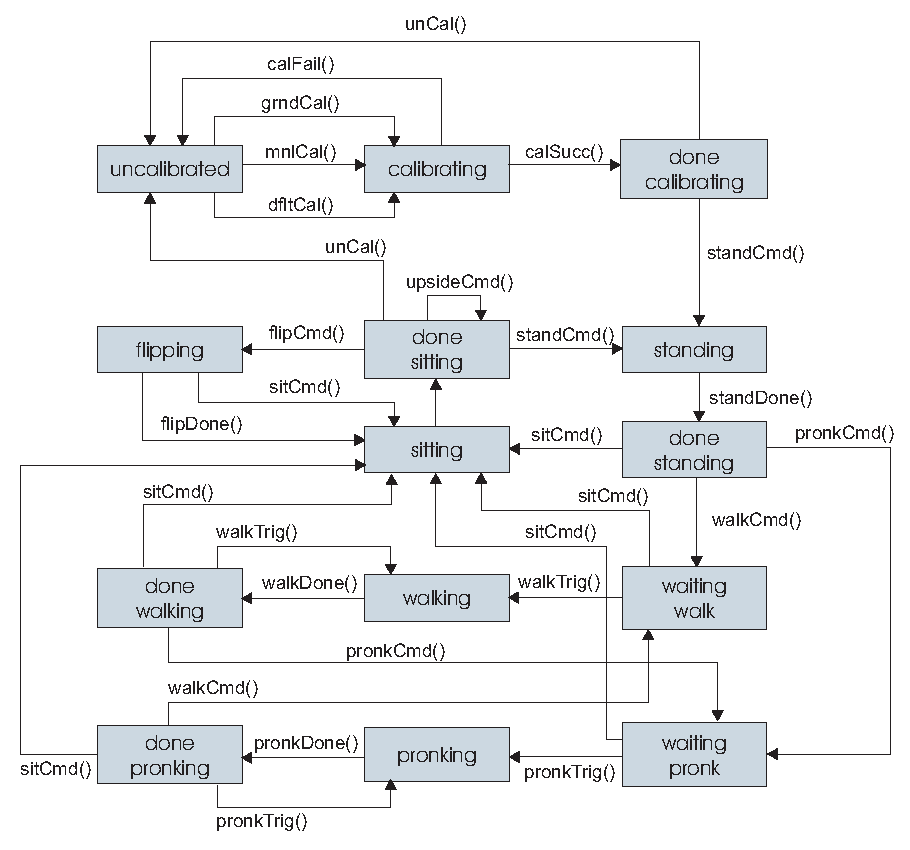
\includegraphics{SupervisorMachine.eps}}
    \caption{State transition diagram for the {\tt Supervisor} state
      machine. This machine controls the overall user interface of the {\tt
        rhex\_standard} demo program.}
    \label{fig:supervisor_machine}
  \end{center}
\end{figure}
%%%%%%%%%%%%%%%%%%%%%%%%%%%%%%%%%%%%%%%%%%%%%%%%


\subsection{The Main Executable}



\input{programming}

\printindex

\end{document}









